%  LaTeX support: latex@mdpi.com 
%  For support, please attach all files needed for compiling as well as the log file, and specify your operating system, LaTeX version, and LaTeX editor.

%=================================================================
\documentclass[sustainability,article,accept,moreauthors,pdftex]{Definitions/mdpi} 
\usepackage[utf8]{inputenc}
\usepackage{listings}
\usepackage{graphics}
\usepackage{graphicx}
\usepackage{subcaption}
\usepackage{mwe}
% For posting an early version of this manuscript as a preprint, you may use "preprints" as the journal and change "submit" to "accept". The document class line would be, e.g., \documentclass[preprints,article,accept,moreauthors,pdftex]{mdpi}. This is especially recommended for submission to arXiv, where line numbers should be removed before posting. For preprints.org, the editorial staff will make this change immediately prior to posting.

%--------------------
% Class Options:
%--------------------
%----------
% journal
%----------
% Choose between the following MDPI journals:
% acoustics, actuators, addictions, admsci, adolescents, aerospace, agriculture, agriengineering, agronomy, ai, algorithms, allergies, analytica, animals, antibiotics, antibodies, antioxidants, appliedchem, applmech, applmicrobiol, applnano, applsci, arts, asi, atmosphere, atoms, audiolres, automation, axioms, batteries, bdcc, behavsci, beverages, biochem, bioengineering, biologics, biology, biomechanics, biomedicines, biomedinformatics, biomimetics, biomolecules, biophysica, biosensors, biotech, birds, bloods, brainsci, buildings, businesses, cancers, carbon, cardiogenetics, catalysts, cells, ceramics, challenges, chemengineering, chemistry, chemosensors, chemproc, children, civileng, cleantechnol, climate, clinpract, clockssleep, cmd, coatings, colloids, compounds, computation, computers, condensedmatter, conservation, constrmater, cosmetics, crops, cryptography, crystals, curroncol, cyber, dairy, data, dentistry, dermato, dermatopathology, designs, diabetology, diagnostics, digital, disabilities, diseases, diversity, dna, drones, dynamics, earth, ebj, ecologies, econometrics, economies, education, ejihpe, electricity, electrochem, electronicmat, electronics, encyclopedia, endocrines, energies, eng, engproc, entropy, environments, environsciproc, epidemiologia, epigenomes, fermentation, fibers, fire, fishes, fluids, foods, forecasting, forensicsci, forests, fractalfract, fuels, futureinternet, futuretransp, futurepharmacol, futurephys, galaxies, games, gases, gastroent, gastrointestdisord, gels, genealogy, genes, geographies, geohazards, geomatics, geosciences, geotechnics, geriatrics, hazardousmatters, healthcare, hearts, hemato, heritage, highthroughput, histories, horticulturae, humanities, hydrogen, hydrology, hygiene, idr, ijerph, ijfs, ijgi, ijms, ijns, ijtm, ijtpp, immuno, informatics, information, infrastructures, inorganics, insects, instruments, inventions, iot, j, jcdd, jcm, jcp, jcs, jdb, jfb, jfmk, jimaging, jintelligence, jlpea, jmmp, jmp, jmse, jne, jnt, jof, joitmc, jor, journalmedia, jox, jpm, jrfm, jsan, jtaer, jzbg, kidney, land, languages, laws, life, liquids, literature, livers, logistics, lubricants, machines, macromol, magnetism, magnetochemistry, make, marinedrugs, materials, materproc, mathematics, mca, measurements, medicina, medicines, medsci, membranes, metabolites, metals, metrology, micro, microarrays, microbiolres, micromachines, microorganisms, minerals, mining, modelling, molbank, molecules, mps, mti, nanoenergyadv, nanomanufacturing, nanomaterials, ncrna, network, neuroglia, neurolint, neurosci, nitrogen, notspecified, nri, nursrep, nutrients, obesities, oceans, ohbm, onco, oncopathology, optics, oral, organics, osteology, oxygen, parasites, parasitologia, particles, pathogens, pathophysiology, pediatrrep, pharmaceuticals, pharmaceutics, pharmacy, philosophies, photochem, photonics, physchem, physics, physiolsci, plants, plasma, pollutants, polymers, polysaccharides, proceedings, processes, prosthesis, proteomes, psych, psychiatryint, publications, quantumrep, quaternary, qubs, radiation, reactions, recycling, regeneration, religions, remotesensing, reports, reprodmed, resources, risks, robotics, safety, sci, scipharm, sensors, separations, sexes, signals, sinusitis, smartcities, sna, societies, socsci, soilsystems, solids, sports, standards, stats, stresses, surfaces, surgeries, suschem, sustainability, symmetry, systems, taxonomy, technologies, telecom, textiles, thermo, tourismhosp, toxics, toxins, transplantology, traumas, tropicalmed, universe, urbansci, uro, vaccines, vehicles, vetsci, vibration, viruses, vision, water, wevj, women, world 

%---------
% article
%---------
% The default type of manuscript is "article", but can be replaced by: 
% abstract, addendum, article, book, bookreview, briefreport, casereport, comment, commentary, communication, conferenceproceedings, correction, conferencereport, entry, expressionofconcern, extendedabstract, datadescriptor, editorial, essay, erratum, hypothesis, interestingimage, obituary, opinion, projectreport, reply, retraction, review, perspective, protocol, shortnote, studyprotocol, systematicreview, supfile, technicalnote, viewpoint, guidelines, registeredreport, tutorial
% supfile = supplementary materials

%----------
% submit
%----------
% The class option "submit" will be changed to "accept" by the Editorial Office when the paper is accepted. This will only make changes to the frontpage (e.g., the logo of the journal will get visible), the headings, and the copyright information. Also, line numbering will be removed. Journal info and pagination for accepted papers will also be assigned by the Editorial Office.

%------------------
% moreauthors
%------------------
% If there is only one author the class option oneauthor should be used. Otherwise use the class option moreauthors.

%---------
% pdftex
%---------
% The option pdftex is for use with pdfLaTeX. If eps figures are used, remove the option pdftex and use LaTeX and dvi2pdf.

%=================================================================
% MDPI internal commands
\firstpage{1} 
\makeatletter 
\setcounter{page}{\@firstpage} 
\makeatother
\pubvolume{1}
\issuenum{1}
\articlenumber{0}
\pubyear{2021}
\copyrightyear{2021}
\externaleditor{Academic Editor: \hl{Firstname Lastname}} % For journal Automation, please change Academic Editor to "Communicated by"
\datereceived{\hl{date}} 
\dateaccepted{\hl{date}} 
\datepublished{\hl{date}} 
\hreflink{https://doi.org/} % If needed use \linebreak
%------------------------------------------------------------------
% The following line should be uncommented if the LaTeX file is uploaded to arXiv.org
%\pdfoutput=1

%=================================================================
% Add packages and commands here. The following packages are loaded in our class file: fontenc, inputenc, calc, indentfirst, fancyhdr, graphicx, epstopdf, lastpage, ifthen, lineno, float, amsmath, setspace, enumitem, mathpazo, booktabs, titlesec, etoolbox, tabto, xcolor, soul, multirow, microtype, tikz, totcount, changepage, paracol, attrib, upgreek, cleveref, amsthm, hyphenat, natbib, hyperref, footmisc, url, geometry, newfloat, caption

%=================================================================
%% Please use the following mathematics environments: Theorem, Lemma, Corollary, Proposition, Characterization, Property, Problem, Example, ExamplesandDefinitions, Hypothesis, Remark, Definition, Notation, Assumption
%% For proofs, please use the proof environment (the amsthm package is loaded by the MDPI class).

%=================================================================
% Full title of the paper (Capitalized)
\Title{Modeling of Combined Lead Fast Reactor and Concentrating Solar Power Supercritical Carbon Dioxide Cycles to Demonstrate Feasibility, Efficiency Gains, and Cost Reductions}

% MDPI internal command: Title for citation in the left column
\TitleCitation{Modeling of Combined Lead Fast Reactor and Concentrating Solar Power Supercritical Carbon Dioxide Cycles to Demonstrate Feasibility, Efficiency Gains, and Cost Reductions}

% Author Orchid ID: enter ID or remove command
\newcommand{\orcidauthorA}{0000-0002-1015-7605} % Add \orcidA{} behind the author's name
\newcommand{\orcidauthorB}{0000-0003-2128-4658} % Add \orcidB{} behind the author's name

% Authors, for the paper (add full first names)
%\dagger -> adds dagger
%\ddagger -> adds double dagger
\Author{\hl{Brian T. White} %Please carefully check the accuracy of names and affiliations. Changes will not be possible after proofreading.
 $^{1}$, Michael J. Wagner~$^{1}$\orcidB{}, Ty Neises~$^{3}$, Cory Stansbury~$^{4}$ and Ben Lindley~$^{2,}$*\orcidA{}}

% MDPI internal command: Authors, for metadata in PDF
\AuthorNames{Brian T. White, Michael J. Wagner, Ty Neises, Cory Stansbury and Ben Lindley}

% MDPI internal command: Authors, for citation in the left column
\AuthorCitation{White, B.T.; Wagner, M.J.; Neises, T.; Stansbury, C.; Lindley, B.}
% If this is a Chicago style journal: Lastname, Firstname, Firstname Lastname, and Firstname Lastname.

% Affiliations / Addresses (Add [1] after \address if there is only one affiliation.)
\address{%
$^{1}$ \quad Department of Mechanical Engineering, University of Wisconsin---Madison, 1415 Engineering Drive, \mbox{Madison, WI 53706, USA;} bwhite24@wisc.edu (B.W.); mjwagner2@wisc.edu (M.W.)\\
$^{2}$ \quad Department of Engineering Physics, University of Wisconsin---Madison, 1500 Engineering Drive, \mbox{Madison, WI 53706, USA}\\
$^{3}$ \quad National Renewable Energy Laboratory, Thermal Systems Group, 15013 Denver West Parkway, \mbox{Golden, CO 80401, USA;} ty.neises@nrel.gov\\
$^{4}$ \quad Westinghouse Electric Company, Lead Fast Reactor Systems Development, 1000 Westinghouse Dr, \mbox{Cranberry Twp, PA 16066, USA;} stansbca@westinghouse.com}

% Contact information of the corresponding author
\corres{Correspondence: lindley2@wisc.edu; Tel.: +1-608-265-2001}

% Current address and/or shared authorship
%\firstnote{Current address: Affiliation 3} 
%\secondnote{These authors contributed equally to this work.}
% The commands \thirdnote{} till \eighthnote{} are available for further notes

%\simplesumm{} % Simple summary

%\conference{} % An extended version of a conference paper

% Abstract (Do not insert blank lines, i.e. \\) 
\abstract{Solar power has innate issues with weather, grid demand and time of day, which can be mitigated through use of thermal energy storage for concentrating solar power (CSP). Nuclear reactors, including lead-cooled fast reactors (LFRs), can %\replaced[comment={Revised sentence for readability [2,1]}]
{adjust power output according to demand; but with high fixed costs and low operating costs, there may not be sufficient economic incentive to make this worthwhile.} %{load follow, but have high fixed and low operating costs which can make this economically unattractive.}  
We investigate potential synergies through coupling CSP and LFR together in a single supercritical CO$_2$ Brayton cycle and/or using the same thermal energy storage. Combining these cycles allows for the LFR to thermally charge the salt storage in the CSP cycle during low-demand periods to be dispatched when grid demand increases.  The LFR/CSP coupling into one cycle is modeled to find the preferred location of the LFR heat exchanger, CSP heat exchanger, sCO$_2$-to-salt heat exchanger (C2S), turbines, and recuperators within the supercritical CO$_2$ Brayton cycle. Three cycle configurations have been studied: two-cycle configuration, which uses CSP and LFR heat for dedicated turbocompressors, has the highest efficiencies but with less component synergies; a combined cycle with CSP and LFR heat sources in parallel is the simplest with the lowest efficiencies; and a combined cycle with separate high-temperature recuperators for both the CSP and LFR is a compromise between efficiency and component synergies. Additionally, four thermal energy storage charging techniques are studied: the turbine positioned before C2S, requiring a high LFR outlet temperature for viability; the turbine after the C2S, reducing turbine inlet temperature and therefore power; the turbine parallel to the C2S producing moderate efficiency; and a dedicated circulator loop. While all configurations have pros and cons, use of a single cycle offers component synergies with limited efficiency penalty. Using a turbine in parallel with the C2S heat exchanger is feasible but results in a low charging efficiency, while a dedicated circulator loop offers flexibility and near-perfect heat storage efficiency but increasing cost with additional cycle components.
}

%{A single paragraph of about 200 words maximum. For research articles, abstracts should give a pertinent overview of the work. We strongly encourage authors to use the following style of structured abstracts, but without headings: (1) Background: place the question addressed in a broad context and highlight the purpose of the study; (2) Methods: describe briefly the main methods or treatments applied; (3) Results: summarize the article's main findings; (4) Conclusion: indicate the main conclusions or interpretations. The abstract should be an objective representation of the article, it must not contain results which are not presented and substantiated in the main text and should not exaggerate the main conclusions.}

% Keywords
\keyword{supercritical carbon dioxide Brayton cycle; concentrating solar power (CSP); lead fast reactor (LFR); cogeneration; complimentary cycle; thermal energy storage (TES)} 
%List three to ten pertinent keywords specific to the article; yet reasonably common within the subject discipline.

% The fields PACS, MSC, and JEL may be left empty or commented out if not applicable
%\PACS{J0101}
%\MSC{}
%\JEL{}

%%%%%%%%%%%%%%%%%%%%%%%%%%%%%%%%%%%%%%%%%%
% Only for the journal Diversity
%\LSID{\url{http://}}

%%%%%%%%%%%%%%%%%%%%%%%%%%%%%%%%%%%%%%%%%%
% Only for the journal Applied Sciences:
%\featuredapplication{Authors are encouraged to provide a concise description of the specific application or a potential application of the work. This section is not mandatory.}
%%%%%%%%%%%%%%%%%%%%%%%%%%%%%%%%%%%%%%%%%%

%%%%%%%%%%%%%%%%%%%%%%%%%%%%%%%%%%%%%%%%%%
% Only for the journal Data:
%\dataset{DOI number or link to the deposited data set in cases where the data set is published or set to be published separately. If the data set is submitted and will be published as a supplement to this paper in the journal Data, this field will be filled by the editors of the journal. In this case, please make sure to submit the data set as a supplement when entering your manuscript into our manuscript editorial system.}

%\datasetlicense{license under which the data set is made available (CC0, CC-BY, CC-BY-SA, CC-BY-NC, etc.)}

%%%%%%%%%%%%%%%%%%%%%%%%%%%%%%%%%%%%%%%%%%
% Only for the journal Toxins
%\keycontribution{The breakthroughs or highlights of the manuscript. Authors can write one or two sentences to describe the most important part of the paper.}

%%%%%%%%%%%%%%%%%%%%%%%%%%%%%%%%%%%%%%%%%%
% Only for the journal Encyclopedia
%\encyclopediadef{Instead of the abstract}
%\entrylink{The Link to this entry published on the encyclopedia platform.}
%%%%%%%%%%%%%%%%%%%%%%%%%%%%%%%%%%%%%%%%%%


% Define fixed-width column types. Use as:
% \begin{tabular}{L{0.5\linewidth}cc}
% ... for example
\newcolumntype{L}[1]%
{>{\raggedright\let\newline\\\arraybackslash\hspace{0pt}}m{#1}}
\newcolumntype{C}[1]%
{>{\centering\let\newline\\\arraybackslash\hspace{0pt}}m{#1}}
\newcolumntype{R}[1]%
{>{\raggedleft\let\newline\\\arraybackslash\hspace{0pt}}m{#1}}


\usepackage[commentmarkup=uwave%
%,final%    <<< uncomment this line to render with changes and remove comments
]{changes}
\usepackage{xspace}
\usepackage{adjustbox}

\definechangesauthor[color=blue!80!black]{MW}
\definechangesauthor[color=red!80!black]{BL}
\newcommand{\mw}[1]{\comment[id=MW]{#1}}
\newcommand{\bl}[1]{\comment[id=BL]{#1}}


% \renewcommand{\added}[1]{\xspace{#1}\xspace}
% \renewcommand{\mw}[1]{\xspace}
% \renewcommand{\bl}[1]{\xspace}
% \renewcommand{\deleted}[1]{\xspace}
% \renewcommand{\replaced}[2]{\xspace{#1}\xspace}



\usepackage{subcaption}

\begin{document}

%
%\section{How to Use this Template}

%The template details the sections that can be used in a manuscript. Note that the order and names of article sections may differ from the requirements of the journal (e.g., the positioning of the Materials and Methods section). Please check the instructions on the authors' page of the journal to verify the correct order and names. For any questions, please contact the editorial office of the journal or support@mdpi.com. For LaTeX-related questions please contact latex@mdpi.com.
%The order of the section titles is: Introduction, Materials and Methods, Results, Discussion, Conclusions for these journals: aerospace,algorithms,antibodies,antioxidants,atmosphere,axioms,biomedicines,carbon,crystals,designs,diagnostics,environments,fermentation,fluids,forests,fractalfract,informatics,information,inventions,jfmk,jrfm,lubricants,neonatalscreening,neuroglia,particles,pharmaceutics,polymers,processes,technologies,viruses,vision

%%%%%%%%%%%%%%%%%%%%%%%%%%%%%%%%%%%%%%%%%%%%%%%%%%%%%%%%%%%%%%%%%%%%%%%%%%%%%%%%%%%%%%%
\section{Introduction}

%The introduction should briefly place the study in a broad context and highlight why it is important. It should define the purpose of the work and its significance. The current state of the research field should be reviewed carefully and key publications cited. Please highlight controversial and diverging hypotheses when necessary. Finally, briefly mention the main aim of the work and highlight the principal conclusions. As far as possible, please keep the introduction comprehensible to scientists outside your particular field of research.  %Please use the command \citep{} for the following MDPI journals, which use author--date citation: Administrative Sciences, Arts, Econometrics, Economies, Genealogy, Histories, Humanities, IJFS, Journal of Intelligence, Journalism and Media, JRFM, Languages, Laws, Religions, Risks, Social Sciences.


Recompression supercritical CO$_2$ Brayton cycles are promising cycle configurations offering higher efficiencies, compact design, and reduced turbomachinery cost while operating with non toxic working fluid. High efficiencies, in some simple recompression cycles reaching 50\% efficiency \cite{turchi_2013,wright_2009}, allows these cycles to be a competitive alternative to steam Rankine and air Brayton cycles over a range of temperatures.
\bl{Updated above as sCO2 can also be used for Coal - it is a cycle vs cycle argument rather than a heat source vs heat source argument -BW}
Various sCO$_2$ Brayton cycles have been modeled with the recompression cycle having the most efficiency advantages over other proposed cycle arrangements \cite{turchi_2013,ahn_2014,wang_2018}.  Due to the benefits of sCO$_2$ Brayton cycles, the United States Department of Energy is investigating these conversion cycles for use with heat sources including nuclear and solar \cite{doe_2012}. Multiple project funding opportunities are established with the National Energy Technology Laboratory offering 144 million dollar reward for demonstration and performance verification of a sCO$_2$ Brayton cycle \cite{netl_2016} and the Office of Energy Efficiency \& Renewable Energy offering 2.6 million dollar reward in their Brayton Energy project for a integrated CSP receiver, TES, and power block in one sCO$_2$ Brayton system \cite{seto_2015}. Utilizing complementary technologies, specifically solar concentrating power and lead-cooled fast reactors, can offset the drawbacks of each. Coupling these technologies into an interconnected cycle allows for consistent generation, independent of weather or time of day, and thermal storage for high dispatchability during high grid demand periods.

\bl{not a big issue but do we want to describe as sCO2 or sCO2 Brayton? In project nomenclature to date I have used sCO2 with the logic that sCO2 'isnt really a Brayton cycle' but both are common -BW}
A CSP has an array of mirrors concentrating solar rays towards a receiver to generate thermal energy therefore causing a dependency on weather conditions and time of day. Previous research has modeled CSP technology as the thermal source for Brayton sCO$_2$ cycles with promising results in efficiency gains and high temperature thermal energy storage \cite{turchi_2013, iverson_2013, ho_2015, wang_2018, neises_2020}. Thermal energy gathered from the CSP is stored in thermal energy storage which is dispatched into the sCO$_2$ Brayton cycle when grid demand increases. With a comparable temperature to the hot TES, 560 $^{\circ}$C, a LFR is capable of transferring heat to thermal storage for later dispatch. An LFR uses fission reactions to heat a heat transfer fluid, in this case liquid lead, to temperatures of 650 $^{\circ}$C. Nuclear sCO$_2$ Brayton cycles have been studied with similar gains in efficiency seen in CSP sCO$_2$ Brayton cycles \cite{ dostal_2004, luo_2020}. Physical testing of simple sCO$_2$ Brayton cycles is researched at Sandia National Labs in Arvada, Colorado, with break-even conditions, where the turbine produces enough power to offset compressor demand, being achieved \cite{wright_2011}. In addition to break-even conditions, research from the Supercritical CO$_2$ Brayton Cycle Integral Experiment Loop, in Korea Atomic Energy Institute, achieved electrical generation in a simple sCO$_2$ Brayton cycle \cite{cha_2016}. 

\bl{I would bullet out the next three citations-BW}
Various studies on complimentary solar-nuclear systems have been accomplished with several reviewed as follows: 

\begin{itemize}
    \item	Monnerie et al. (2011): In search of an alternative to the typical fossil fuel-based process, reports on synthesizing hydrogen with complimentary solar-nuclear technologies being utilized as consistent heat sources for chemical decomposition of sulphuric acid to aid in simple, low-temperature electrolysis \cite{monnerie_2011}. 
    \item   Curtis J.D. (2015): Massachusetts Institute of Technology thesis reports cycle configuration, performance, and development of complimentary solar-nuclear systems with a focus on shale oil extraction and production from kerogen deposits \cite{curtis_2015}. 
    \item   Wang et al. (2020): Implements a combined solar and nuclear plant discussing a sCO$_2$ Brayton recompression cycle layout with an emphasis on a cycle design's performance to varying solar irradiance and demonstration of feasibility \cite{wang_2020}. 
\end{itemize}

The economic and physical feasibility of producing shale oil and hydrogen with complimentary solar-nuclear cycles, as discussed in the Curtis J.D. (2015) thesis and Monnerie et al. (2011) article, is not within the scope of sCO$_2$ Brayton recompression cycle electrical generation and storage presented in this paper.

The single cycle configuration in Wang et al. (2020) has a higher-temperature operating salt, 67\%KCl-33\%MgCl$_2$, as the heat transfer fluid in the CSP which is capable of temperatures in the range of 450 - 1400 $^{\circ}$C. The lower operating point of the studied solar salt in this paper, 60\%NaNO$_3$-40\%KNO$_3$ with a temperature range of 250 - 585 $^{\circ}$C, is employed because the technology is more established when compared to KCl-MgCl$_2$ \cite{turchi_2018}. The higher temperature salt requires preheating which is achieved prior to the CSP heat addition by a small modular lead-cooled fast reactor. The small modular LFR operates at a low temperature and a fixed location when compared to the higher temperature lead and variable location that the Westinghouse LFR studied in this paper is capable of. Due to the similar operating temperatures of the CSP and LFR, multiple cycle configurations are studied that are not possible with the similar components in Wang et al. (2020). Specifically studied in this paper are the effects on cycle and heat storage efficiency of different cycle configurations while having the LFR serve a dual purpose of electrical generation and a supplementary CSP TES charging technique. This paper provides an overview of contending recompression sCO$_2$ Brayton cycles with varied positioning of complimentary CSP and LFR heat additions in the cycle. Additionally the location of where heat is drawn from the sCO$_2$ Brayton cycles to be stored in thermal energy storage is studied with the results discussed.


%Monnerie et al. (2011), in search of an alternative to the typical fossil fuel-based process, reports on combining nuclear and solar energy in the same plant to produce hydrogen \cite{monnerie_2011}.  Extraction and production of fuels using complimentary solar-nuclear systems is additionally studied in the Curtis 2015 thesis from Massachusetts Institute of Technology where cycle configuration, performance, and development of shale oil extraction from kerogen deposits is reported \cite{curtis_2015}. Utilizing complimentary solar-nuclear cycles for production of hydrogen or shale oil with economical feasibility of the system discussed, in contrast to a fucus on electrical generation and storage in a sCO$_2$ Brayton recompression cycle, is not within the scope of the presented research in this paper.

%Implementation of a combined solar and nuclear plant, modeled in the Wang et al. (2020) shows a single sCO$_2$ Brayton recompression cycle layout with an emphasis on a cycle design's performance to varying solar irradiance and demonstration of feasibility \cite{wang_2020}.  This single cycle configuration has a dissimilar higher-temperature operating salt, KCl-MgCl$_2$, as the heat transfer fluid in the CSP with the small modular lead-cooled fast reactor's main purpose as a preheater to the CSP heat addition instead of being utilized as an TES charging alternative. Presented in this paper are the effects on cycle and heat storage efficiency of alternative heat addition locations while having the LFR serve a dual purpose of electrical generation and a supplementary CSP TES charging technique. 
%This paper will provide an overview of contending recompression sCO$_2$ Brayton cycles with varied positioning of complimentary CSP and LFR heat additions in the cycle. Additionally the location of where heat is drawn from the sCO$_2$ Brayton cycles to be stored in thermal energy storage is studied and the results discussed.
\bl{I think the last citation merits its own paragraph and a little further discussion (1-2 more sentences). You could start by saying that it is prior work on the LFR-CSP-sCO2 concept. Then describe its cycle configuration with the high temperature salt. Then in the following sentence (the stuff you currnetly have highlighted) you can say that your work is investigating higher lead temperatures than Wang (because of Westinghouse LFR) and lower temperature salt (technology readiness) and this leads to very different cycle configurations and options than Wang, as will be discussed. The overall tone is that you work recognizes and builds on Wang, rather than needing to justify its existance despite Wang - BW}


 
%%%%%%%%%%%%%%%%%%%%%%%%%%%%%%%%%%%%%%%%%%%%%%%%%%%%%%%%%%%%%%%%%%%%%%%%%%%%%%%%%%%%%%%
\section{Materials and Methods}

%Materials and Methods should be described with sufficient details to allow others to replicate and build on published results. Please note that publication of your manuscript implicates that you must make all materials, data, computer code, and protocols associated with the publication available to readers. Please disclose at the submission stage any restrictions on the availability of materials or information. New methods and protocols should be described in detail while well-established methods can be briefly described and appropriately cited.

%Research manuscripts reporting large datasets that are deposited in a publicly avail-able database should specify where the data have been deposited and provide the relevant accession numbers. If the accession numbers have not yet been obtained at the time of submission, please state that they will be provided during review. They must be provided prior to publication.

%Interventionary studies involving animals or humans, and other studies require ethical approval must list the authority that provided approval and the corresponding ethical approval code.
%\begin{quote}
%This is an example of a quote.
%\end{quote}

% **************************************

%MW: I've fixed spelling in a few places. You can install a spell checker to highlight misspelled words. I use the "Code spell checker" extension.


\subsection{Cycle Component Modeling}
%======================================================================================
Components present in the cycles are modeled using various techniques and are discussed in more detail below. Turbines and compressors are analyzed using isentropic efficiencies. Counter-flow heat exchangers are modelled using the effectiveness-NTU method while simplified ``black box'' heat exchangers that use a simple energy balance for state point calculations are used in lieu of more detailed component models where data is available. The lead-cooled fast reactor is assumed to be a black box heat exchanger because of the constant heat input and state points on the sCO$_2$ inlet and outlet are provided. The concentrating solar power cycle is modeled with necessary components including hot and cold TES, receiver, pumps and counter-flow heat exchangers.



\subsubsection{Turbines and Compressors }
%--------------------------------------------------------------------------------------

Turbines and compressors are modeled for each cycle using constant isentropic efficiency values which are summarized in Table \ref{tab-cycle-constants}. Turbines take the high pressure sCO$_2$ and expand it through a series of blades allowing a production of energy, while compressors input mechanical energy to increase the pressure of the sCO$_2$. The turbines and compressors are assumed to be at steady state, exchange no heat with the surroundings, and have single inlet and outlet streams. Using this estimate, along with a known low and high side pressures, temperature and enthalpy outlets of the turbine and compressor are calculated \cite{klein_nellis_2011}. 

%Power calculations are initially done on ideal, reversible compressors or turbines then are scaled by the isentropic efficiencies to provide an estimate for a realizable component.\mw{this is kind of an awkward way to describe what's happening. I think most readers are familiar with isentropic efficiencies and this can be omitted.}

\subsubsection{Black Box and Counter-Flow Heat Exchangers}
%--------------------------------------------------------------------------------------

Black box heat exchangers are simplified heat exchangers which have no approach temperature or pinch point and are modeled as a perfect heat transfer into or out of the cycle. These heat exchangers use an energy balance with mass flow inlet energy, heat input or output, and mass flow outlet energy. The energy balance equation used for all black box heat exchangers is Equation \ref{eq-black}.

%\mw{This is for a single flow stream. Why would there be $\dot{Q}_{in}$ and $\dot{Q}_{out}$ in a single flow stream? Also, the variable should be consistent with the figure, which would be $\dot{Q}_{HX}$. -BW}


\begin{equation}
    \label{eq-black}
    \dot{m} \cdot h_{in} + \dot{Q}_{HX} = \dot{m} \cdot h_{out} ,
\end{equation}

In this equation the energy input to the system is on the left hand side with $\dot{m}$ multiplied by $h_{in}$ being energy from the mass flow while $\dot{Q}_{HX}$ is heat transfer directly into, positive, or out of, negative, the flow from an outside source. The right hand side of the equation is heat leaving the black box heat exchanger with $\dot{m}$ and enthalpy of $h_{out}$. Black box energy balances are used in three situations, the receiver, LFR heat exchanger, and PC heat exchanger. These heat exchangers are not exhaustively modeled because the state points on the inlet and outlet are defined by design parameters.

Counter-flow heat exchangers are modeled with two fluids flowing in opposite directions exchanging heat from the hot side to the cold side. The temperatures of the hot and cold flows on either side of the the heat exchanger have a temperature difference known as an approach temperature. A diagram showing a simplified counter-flow heat exchanger is illustrated in Figure \ref{counter-flow-hx}.

\end{paracol}
\begin{figure}[H] 
    \widefigure
    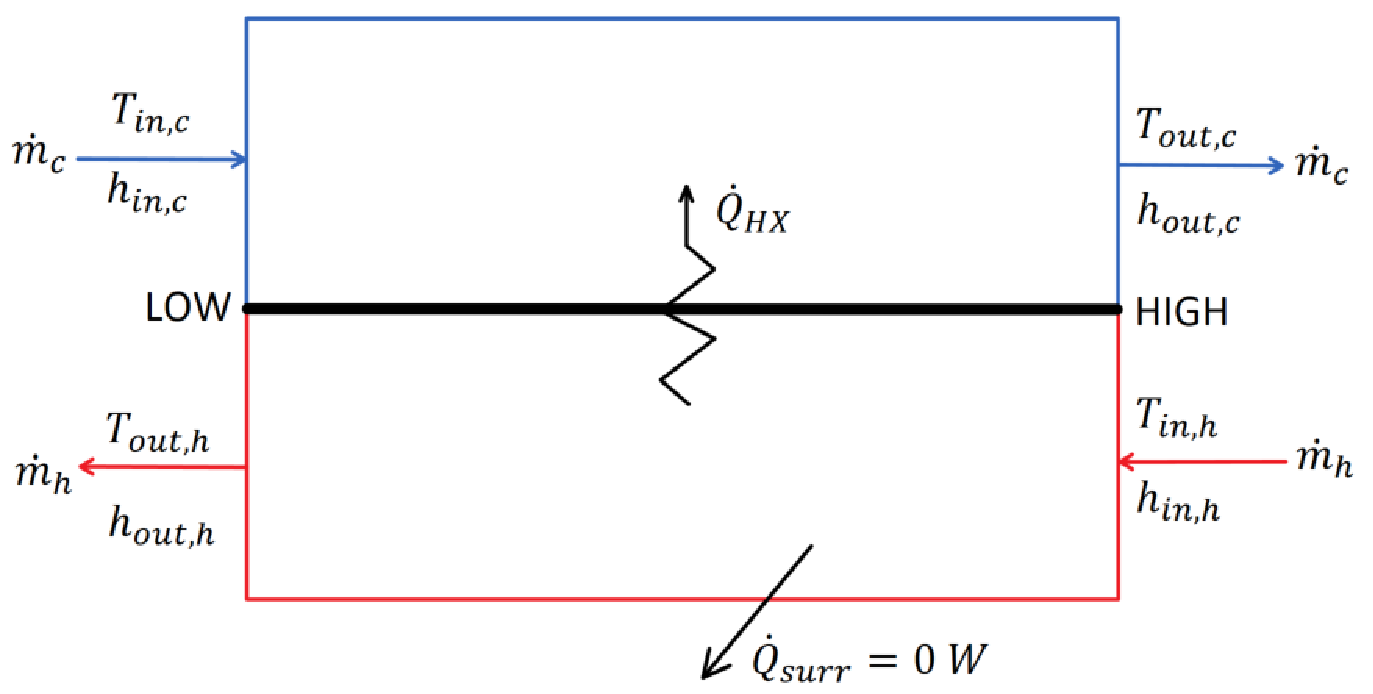
\includegraphics[width=10 cm]{Definitions/counter-flow-hx.pdf}
    \caption{Simple counter-flow heat exchanger diagram. \label{counter-flow-hx}}
\end{figure}
\begin{paracol}{2}
\linenumbers
\switchcolumn

Additional assumptions of the counter-flow heat exchanger model are: no heat loss to the surroundings, no pressure drops across the heat exchangers, and no fouling resistances. In Figure \ref{counter-flow-hx} the subscript 'out' denotes where the streams are leaving, 'in' denotes the entering streams, 'c' and 'h' signify cold and hot streams respectively, $\dot{Q}_{HX}$ is the total heat transfer from the hot to cold stream, and $\dot{Q}_{surr}$ is the heat transfer to the surroundings.

Counter-flow heat exchanger calculations require two known state points, fluid libraries, mass flow rate of hot and cold side, and a specified approach temperature. In the modeled cases, the approach temperature is set to value of $10^{\circ}$C, based off prior model development of sCO$_{2}$ Brayton cycle heat exchangers \cite{seidel_2010_model_development}. The fluid libraries referenced are built into EES for Carbon Dioxide and Salt (60\% NaNO$_3$ 40\% KNO$_3$) \cite{pacheco_1995_salt_properties,roland_1996_co2_properties}. 

To analyze the counter-flow heat exchanger a side is chosen, usually the high side, to start the calculations. The approach temperature is initially subtracted from the hot stream on the high temperature side to find the missing cold temperature according to Equation \ref{temp_h}. 

\begin{equation}
   \label{temp_h}
    T_{out,c} = T_{in,h}-\Delta_{T},
\end{equation}

Where T$_{out,c}$ is the cold stream outlet temperature and T$_{in,h}$ is the hot stream inlet temperature. Knowing the two state points allows for the enthalpy out to be found using correlations from the fluid property libraries. This enthalpy then allows for the heat transfer of the heat exchanger to be found with Equation \ref{heattrans_h}.

\begin{equation}
    \label{heattrans_h}
     \dot{Q}_{HX} = \dot{m}_{c}(h_{out,c}-h_{in,c}),
 \end{equation}

 Where $\dot{Q}_{HX}$ is the total heat transfer rate from the hot stream to the cold stream, $\dot{m}_{c}$ is the mass flow rate of the cold stream, $h_{out,c}$ is the enthalpy at the outlet of the cold side, and $h_{in,c}$ is the inlet of the cold side.
 The known heat transfer of the counter-flow heat exchanger can then solve for the enthalpy out of the hot stream, h$_{out,h}$. This is accomplished with Equation \ref{enthalpy_h}.

 \begin{equation}
    \label{enthalpy_h}
     h_{out,h} = h_{in,h} - \frac{\dot{Q}_{HX}}{\dot{m}_{h}},
 \end{equation}

Knowing the hot stream enthalpy out allows for all states to be set on the outlets and inlets of the counter-flow heat exchanger. The temperature difference of the low side is then checked to ensure that it is larger than the approach temperature, defined at $10^\circ$C. If the temperature difference on the low side is smaller than the approach temperature, the same computations are carried with the low side as the starting point.

Knowing the state points on all inlets and outlets of the counter-flow heat exchanger allows for the heat exchanger performance metrics to be calculated. Performance metrics include effectiveness, capacitance ratio, UA, and NTU for heat exchangers. Effectiveness is the ratio of the actual heat transfer rate to the maximum heat transfer rate, or a perfect heat exchanger with no approach temperature. Assuming the approach temperature is on the high side, the maximum heat transfer rate, $\dot{Q}_{max}$ is found with the maximum enthalpy. Maximum enthalpy of the cold stream is found with correlations by setting the temperature to T$_{in,h}$ with same pressure on the cold outlet. Using the maximum enthalpy, $h_{max}$, the maximum heat transfer rate is calculated using Equation \ref{heattrans_max}.

\begin{equation}
    \label{heattrans_max}
    \dot{Q}_{max} = \dot{m}_{c}(h_{max}-h_{in,c}),
\end{equation}

Calculating the maximum heat transfer rate allows for effectiveness to be calculated using the ratio in Equation \ref{effective}.

\begin{equation}
    \label{effective}
    \varepsilon = \frac{\dot{Q}_{HX}}{\dot{Q}_{max}},
\end{equation}

All of the prior equations are carried out in a built-in function within EES. EES is an iterative solver, therefore as long as there is a feasible solution, the functions can take any of the four state points around the heat exchanger and converge on a solution.

After the effectiveness is solved for, capacitance ratio is necessary. The capacitance ratio is defined as the average minimum capacitance rate, $\dot{C}_{min}$, over the average maximum capacitance rate, $\dot{C}_{max}$. Average capacitance rates for the hot and cold streams are found by multiplying the addition of the specific heat at the inlet and outlet of the stream by the mass flow and dividing by two as seen in Equation \ref{avg_cap}.

\begin{equation}
    \label{avg_cap}
    \dot{C}_{avg} = \frac{\dot{m}(c_{in}+c_{out})}{2},
\end{equation}

Where $C_{avg}$ is the average capacitance rate across the hot or cold stream and $c_{in}$ and $c_{out}$ is the specific heat at the inlet and outlet respectively. Specific heat is found using library correlations. Once both average capacitances are calculated for the hot and cold streams, one has a larger value, $\dot{C}_{max}$, and one has a smaller value,  $\dot{C}_{min}$. These maximum and minimum values are used to find the capacitance ratio, $CR$, in Equation \ref{cap_ratio}.

\begin{equation}
    \label{cap_ratio}
    CR = \frac{\dot{C}_{min}}{\dot{C}_{max}},
\end{equation}

Using values of effectiveness and capacitance ratio, the effectiveness-NTU method can be employed to find the number of transfer units, $NTU$, and the conductance, $UA$ \cite{klein_nellis_2011,nellis_klein_2008}. 



\subsubsection{Lead-Cooled Fast Reactor}
%--------------------------------------------------------------------------------------
Lead-cooled fast reactors use energy from a controlled nuclear reaction to heat molten lead. This lead is used to cool the core and transfer heat into the sCO$_2$ Brayton power cycle \cite{smith_2016_lfr_background,alemberti_2013_lfr_overview}. The lead-cooled fast reactor is assumed to be a black box heat transfer and is labeled in the cycle models LFR HX. The inlet, outlet and heat transfer rates are provided by our industry partner, Westinghouse, making the black box simplification viable. The energy balance for the black box assumption can be seen in Equation \ref{eq-lfr-black-box}.

\begin{equation}
    \label{eq-lfr-black-box}
    \dot{m} \cdot h_{inlet} + \dot{Q}_{LFRHX} = \dot{m} \cdot h_{outlet},
\end{equation}

%\mw{If mass is conserved, use a single $\dot{m}$ - BW}

Where the left hand side, $\dot{m}$, $h_{inlet}$, and $\dot{Q}_{LFRHX}$, is the energy into the flow and the right hand side, $\dot{m}$ and $h_{outlet}$, is the energy brought out from the flow of sCO$_2$. The amount of energy transferred into the cycle, $\dot{Q}_{LFRHX}$, is set at $950$ MW, and outlet temperature of the sCO$_2$ from the LFR HX is set at a value of $595^{\circ}$C. 
%\mw{Make sure numbers are in math mode -BW}
The outlet temperature of the LFR is specified, accounting for the high temperature material limits on the LFR lead side. LFR sCO$_2$ inlet low temperature has a lower bound of $340^{\circ}$C and an optimal value of $400^{\circ}$C, as provided by Westinghouse.
%\mw{How do we know that 400C is the optimal temperature? This information is given to us by Westinghouse, right? -BW} 
\bl{In an LFR, the outlet temperature is limited by materials considerations. The flow velocity is limited by erosion of the fuel (if the lead gets too fast, it erodes the fuel). We want the core to be compact. Therefore the mass flow is limited. This means that a lower inlet temperature gives a higher power (subject to constraints on fuel temperautre, which is also a function of power density). There is a limit of about 340C, below which the lead might freeze (which is operationally unacceptable), but until that value, lower inlet = higher core power. However, from thermodynamics, higher inlet = higher efficiency. There is a trade-off between driving the core harder and getting better cycle performance. The trade-off gives 400C as a temperature that doesnt overly compromise core power while still providing reasonable efficiency. Raising this temperature higher would drop the core power below the 950 MW}
Increasing the sCO$_2$ LFR inlet temperature above this optimal value leads to diminishing returns on the LFR efficiency.


\subsubsection{Concentrating Solar Power Cycle}
%--------------------------------------------------------------------------------------

The CSP salt cycle modeled in this paper is composed of hot and cold thermal energy storage (TES), pumps, receiver, sCO$_2$-to-salt counter-flow heat exchanger (C2S), and CSP counter-flow heat exchanger (CSP HX). The diagram for this CSP salt cycle is seen in Figure \ref{csp}. 

%\mw{Best practice is to allow figures to float. To do this, specify the location as [htb] ("here, top, or bottom"). I've done a search-replace for all figures to do this. -BW}

% \end{paracol}


\begin{figure}[H] 
    %[htb]
    \widefigure
    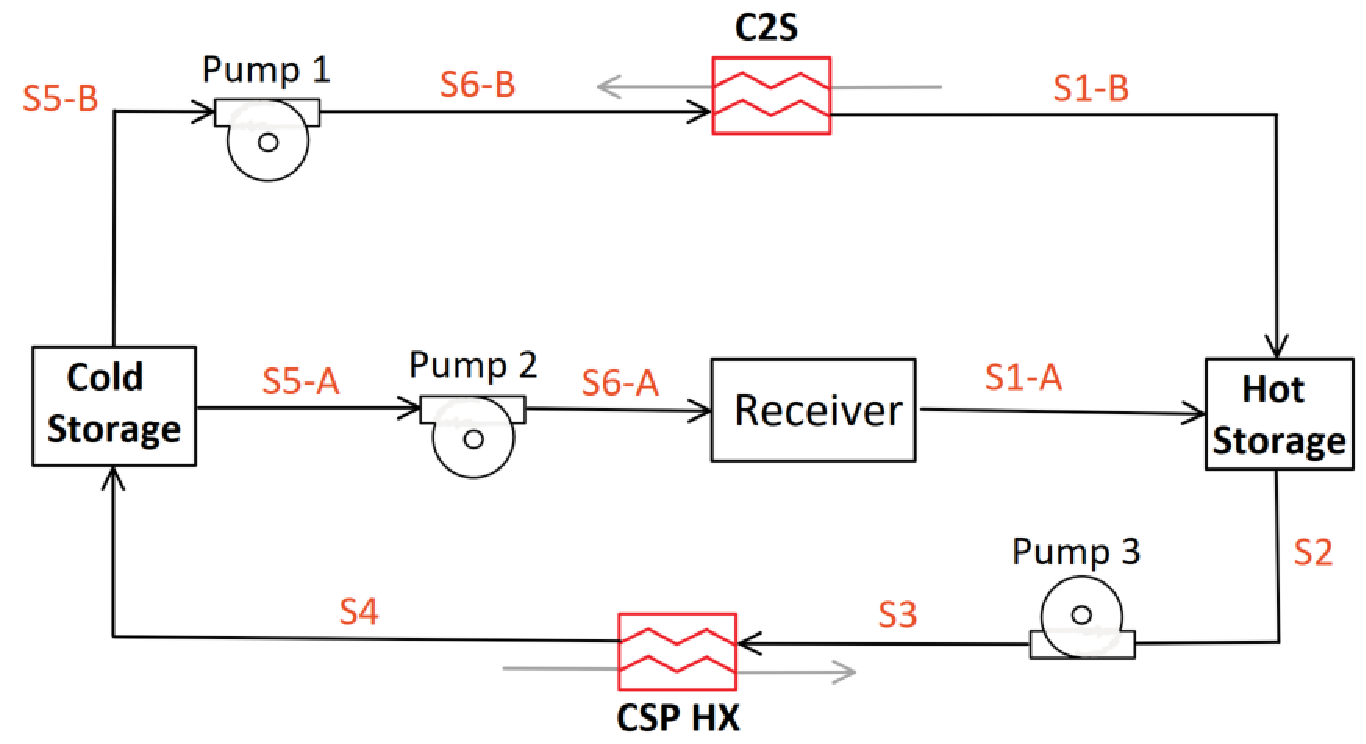
\includegraphics[width=10 cm]{Definitions/csp.pdf}
    \caption{Diagram for CSP cycle with cold and hot thermal energy storage, pumps, and csp black box heat input\label{csp}}
\end{figure}
% \begin{paracol}{2}
% \linenumbers
% \switchcolumn

The CSP salt cycle uses 60\% sodium nitrate, NaNO$_3$, and 40\% potassium nitrate, KNO$_3$, 'solar salt' as the heat transfer fluid. Solar salt stored in the hot TES can be dispatched on demand through the CSP HX when grid demand increases and held when grid demand is low. Current CSP salt cycles heat solar salt with receivers and store it in hot TES tanks at temperatures around 565$^{\circ}$C. Future CSP salt cycles are hypothesized to have bulk hot TES temperatures of up to 720$^{\circ}$C, but due to high temperature limitations with the LFR outlet, the hot TES temperature is set at 560$^{\circ}$C for all modeled cycles \cite{mehos2017concentrating}. The cold TES temperature takes on three different values according to cycle configuration capabilities: 390$^{\circ}$C, 410$^{\circ}$C, and 440$^{\circ}$C. In addition to the lower hot TES temperature, current CSP salt cycles lack a secondary option for charging the hot TES \cite{hamilton2020dispatch}. The studied CSP salt cycle has two TES charging options: a receiver, which generates heat from a heliostat field, and C2S heat exchanger, which draws excess heat from the sCO$_2$ Brayton cycle. While the hot TES is charging, the receiver and LFR are storing heat for later use when grid demand increases. The hot TES storage is not dispensing salt for use in the CSP cycle while charging.

The C2S heat exchanger is active in the 'charging' cycle operating modes, when the focus is on heat storage for later use. Pump 1 is actively moving solar salt from cold TES to hot TES through the C2S heat exchanger extracting heat from the sCO$_2$ Brayton cycle. Additionally, while the focus is on heat storage, and the heliostat field is inputting heat, pump 2 is actively transporting solar salt through the receiver to be stored in the hot TES.
%\mw{Is this necessarily true? Couldn't there be a condition where we'd like to dump energy from the LFR while simultaneously collecting from CSP? } 

'Non-charging' cycle operating modes are characterized by operations wherein the CSP salt cycle is discharging the hot TES, the C2S heat exchanger is not transferring heat, and the LFR is dispatching heat directly to generate electricity. When electrical generation is occurring, the heat input in the CSP salt cycle is modelled through a black box energy balance across states S6-A and S1-A with a heat addition of 750 MW from the heliostat field. The hot TES solar salt is moved through Pump 3 and transfers heat into the sCO$_{2}$ Brayton cycle through CSP HX to be converted into electricity. The cooled salt is stored in cold storage and moved through Pump 2 where the heat from the receiver is again transferred into the CSP cycle. 

When grid demand for electrical power increases, a series of operating modes are activated. During the highest demand times, cycle operation focuses on maximum electrical generation. This is achieved through the C2S being turned off for direct electrical production from the LFR and the hot TES is discharging heat through the CSP HX for electrical production in the sCO$_2$ Brayton cycle. As grid demand diminishes, CSP HX ramps down heat extraction until no power is being dispatched through the salt and the hot TES begins charging. During this process, the LFR gradually adds a larger fraction of heat input to the TES through C2S. This process continues until no electrical production is occurring in the cycle and all heat is stored in TES for later use.

\bl{I dont think the above covers the case where the salt discharges. It might be worth eliciting how the operating modes change as power demand increases. From highest to lowest demand. In all modes CSP will charge the salt is sun is available: (1) LFR and S2C both dispatch, maximum power (2) As power demand decreases, S2C ramps down until no power dispatched through salt (i.e. salt is charged) (3) LFR dispatches, no dispatch from S2C (4) LFR ramps down and gradually transfers greater and greater fraction of power to salt using C2S. (5) No electricity dispatched, all LFR heat passes through C2S -BW
}



\subsection{Standardization of Cycle Modeling}
%======================================================================================
%\mw{What do you mean by ``generalized?''-BW}

In order to draw a more direct comparison, the cycles are standardized in terms of isentropic efficiencies, heat exchanger approach temperatures, pressures, heat input, and pump constants. These values are summarized in Table \ref{tab-cycle-constants}.

\begin{specialtable}[H] 
    %[htbp]
    %\mw{Also changing the specialtable position to allow latex to better place tables.-BW}
    \caption{Standardized constant cycle parameters with definition, variable and set value. \label{tab-cycle-constants}}
    \begin{tabular}{L{0.5\linewidth}cc}
    \toprule
    \textbf{Parameter} & \textbf{Variable}	& \textbf{Design Point Value}\\
    \midrule
    \textit{Efficiencies}\\
    Main Compressor & $\eta_{MC}$		& 0.91 (-)\\
    Re-Compressor & $\eta_{RC}$		& 0.89 (-)\\
    Turbine & $\eta_{T}$		& 0.90 (-)\\
    Pumps 1-3 & $\eta_{P}$      & 0.90 (-)\\
    \midrule
    \textit{Approach Temperatures}\\
    Low Temperature Recuperator & $\delta_{LTR}$		& 10 ($^{\circ}$C)\\
    High Temperature Recuperator & $\delta_{HTR}$		& 10 ($^{\circ}$C)\\
    Concentrating Solar Power Heat Exchanger & $\delta_{CSPHX}$	& 10 ($^{\circ}$C)\\
    \midrule
    \textit{Pressures}\\
    Pressure Ratio & $PR$ & 3.27 (-)\\
    High Side Pressure & $P_{2A}$ & 28.8 (MPa)\\
    \midrule
    \textit{Heat Into System}\\
    Lead-Cooled Fast Reactor Heat Transfer & $\dot{Q}_{LFRHX}$ & 950 (MW)\\
    Concentrating Solar Power Heat Transfer & $\dot{Q}_{CSP}$ & 750 (MW)\\
    \midrule
    \textit{Temperature}\\
    Main Compressor Inlet & $T_{1A}$ & 40 ($^{\circ}$C)\\
    %Lead-Cooled Fast Reactor sCO$_{2}$ Low Temperature & $T_{4}$,$T_{1C}$,$T_{5A}$,$T_{4C}$ & 673.2 (K)\\
    Lead-Cooled Fast Reactor sCO$_{2}$ High Temperature & $T_{5}$,$T_{2C}$,$T_{6A}$,$T_{5C}$ & 595 ($^{\circ}$C)\\
    \midrule
    \textit{Pumps}\\
    Pressure Rise Across Pump & $\Delta_{P}$ & 3.726 (MPa)\\
    Pump Low Side Pressure & $P_{S5-B}$ & 3 (MPa)\\ 
    \bottomrule
    \end{tabular}
\end{specialtable}

The values displayed in Table \ref{tab-cycle-constants} are representative of LFR and CSP design while being consistent with design parameters given by our industry partner, Westinghouse Electric Company. 


In addition to standardized parameters, all cycles have identical recompression sides. The recompression side contains a precooler, low temperature recuperator, and two compressors; main compressor and recompressor. 
\mw{We need an overview here of our process for identifying which cycles will be modeled, as the discussion below gets a bit complicated with all of the different permutations. It might be helpful to have a model taxonomy that schematically shows how the different models are related to each other.}
%\mw{components don't need to be capitalized -- they aren't proper nouns -BW}

Modeled cycles are summarized in Table \ref{tab-cycle_sum}.

\begin{specialtable}[H] 
    \caption{Summary of all modeled non-charging and charging cycles with descriptions. \label{tab-cycle_sum}}
    \begin{tabular}{lL{0.7\linewidth}}
    \toprule
    \textbf{Cycle Label} & \textbf{Description}\\
    \midrule
    \textit{Non-Charging}\\
    C-LFR-ON & Two-cycle configuration with LFR as heat source.\\
    C-CSP-ON & Two-cycle configuration with CSP as heat source.\\
    C-1HTR1T-ON & CSP and LFR heat sources in parallel with one turbine.\\
    C-2HTR3T-ON & CSP and LFR loops each with dedicated HTR and turbine.\\
    \midrule
    \textit{Charging}\\
    C-LFR-PRE & Turbine is prior to the C2S.\\
    C-LFR-POST & Turbine is after the C2S.\\
    C-LFR-PAR & Turbine is parallel to the C2S.\\
    C-LFR-CIRC & Circulator bridges the LFR and C2S.\\
    \bottomrule
    \end{tabular}
\end{specialtable}

\subsection{Non-Charging Cycle Configurations} 
%======================================================================================

Various cycles are modeled to test their advantages and disadvantages. These cycle models fall into two categories: non-charging and charging. The non-charging category is used to determine the configuration of the cycle with a focus on electricity generation. This includes the number and location of turbines, recuperators, and heat input to the system by the CSP and LFR. To quantify the effectiveness of the non-charging configurations, a cycle efficiency, $\eta_{cycle}$, is defined in Equation \ref{eq-eta-cycle}.

\begin{equation}
    \label{eq-eta-cycle}
    \eta_{cycle} = \frac{\dot{W}_{T}-\dot{W}_{MC}-\dot{W}_{RC}}{\dot{Q}_{LFRHX}+\dot{Q}_{CSPHX}},
\end{equation}

The numerator in Equation \ref{eq-eta-cycle} is the alternator power, or the power produced from the turbines, $\dot{W}_{T}$, minus the required power of the compressors, $\dot{W}_{MC}$ and $\dot{W}_{RC}$. The denominator is the total power input into the system from the LFR HX, $\dot{Q}_{LFRHX}$, and CSP HX, $\dot{Q}_{CSPHX}$.


\subsubsection{Two-Cycle Configuration: C-LFR-ON and C-CSP-ON} %--------------------------------------------------------------------------------------

The two-cycle configuration that is tested has independent sCO$_{2}$ loops that share a common CSP salt cycle. This cycle has two sCO$_{2}$ Brayton Cycles: C-LFR-ON and C-CSP-ON. Configuration of components for these two cycles is identical with the exception of heat inputs. C-LFR-ON has heat provided from a LFR while C-CSP-ON has heat provided from the CSP. These two cycles individually operate when the focus of plant operation is primarily electricity generation. 
    
The cycle that is using the LFR heat input in the two-cycle configuration is labeled as C-LFR-ON and the cycle diagram is illustrated in Figure \ref{c-lfr-on}. 
%\mw{There are lots of little 1-2 sentence ``paragraphs'' that could be consolidated with some thought.}

\end{paracol}
\begin{figure}[H] 
    %[!h] 
    \widefigure
    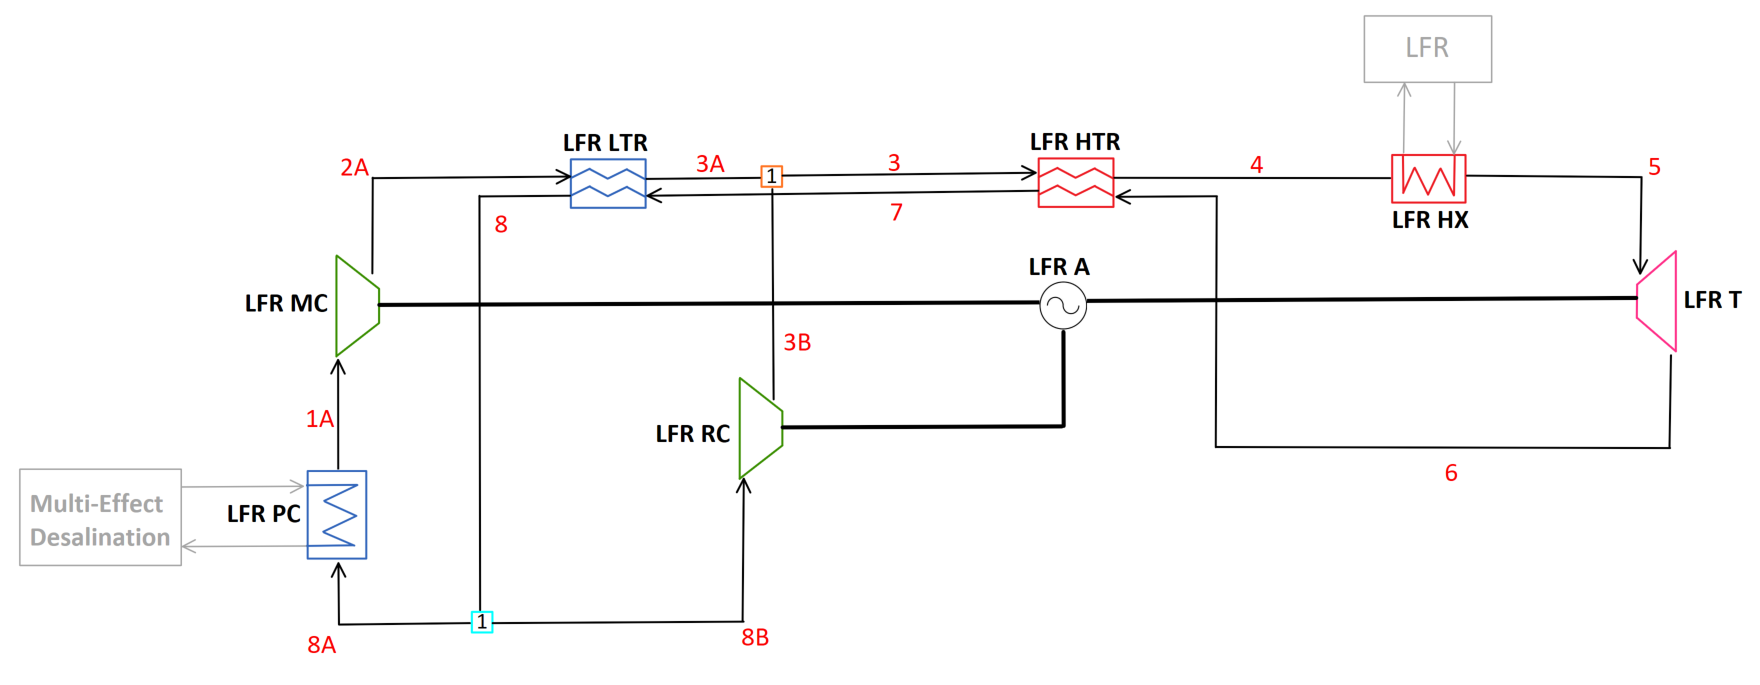
\includegraphics[width=\linewidth]{Definitions/c-lfr-on.pdf}
    \caption{Diagram for C-LFR-ON with focus on electricity generation\label{c-lfr-on}}
\end{figure}
\begin{paracol}{2}
\linenumbers
\switchcolumn

Two separate sensitivity studies on the LFR inlet temperature are completed for C-LFR-ON. The constrained study is calculated by setting the LFR inlet temperature to the design value of $400^{\circ}$C, which is a requirement of the LFR primary circuit to maximize power output within material limits. In addition to the constrained studies, unconstrained studies are required to test the penalties that LFR inlet temperature has on efficiency. The unconstrained study is performed by gradually increasing the mass flow to the main compressor through a parametric study while maximizing cycle efficiency. In Figure \ref{c-lfr-on}, the location of the C2S heat exchanger while charging falls between state point 5 and 6 in any of the studied charging configurations: parallel, pre, circulator or post. 
%%\bl{flip the order of this para: constrained then unconstrained. State that the unconstrained is a 'sensitivty' case to determine the penalty of the constraint}

The cycle that is using the CSP heat input in the two-cycle configuration is labeled C-CSP-ON and the cycle diagram is shown in Figure \ref{c-csp-on}. 

\end{paracol}
\begin{figure}[H] 
    %[!h]
    \widefigure
    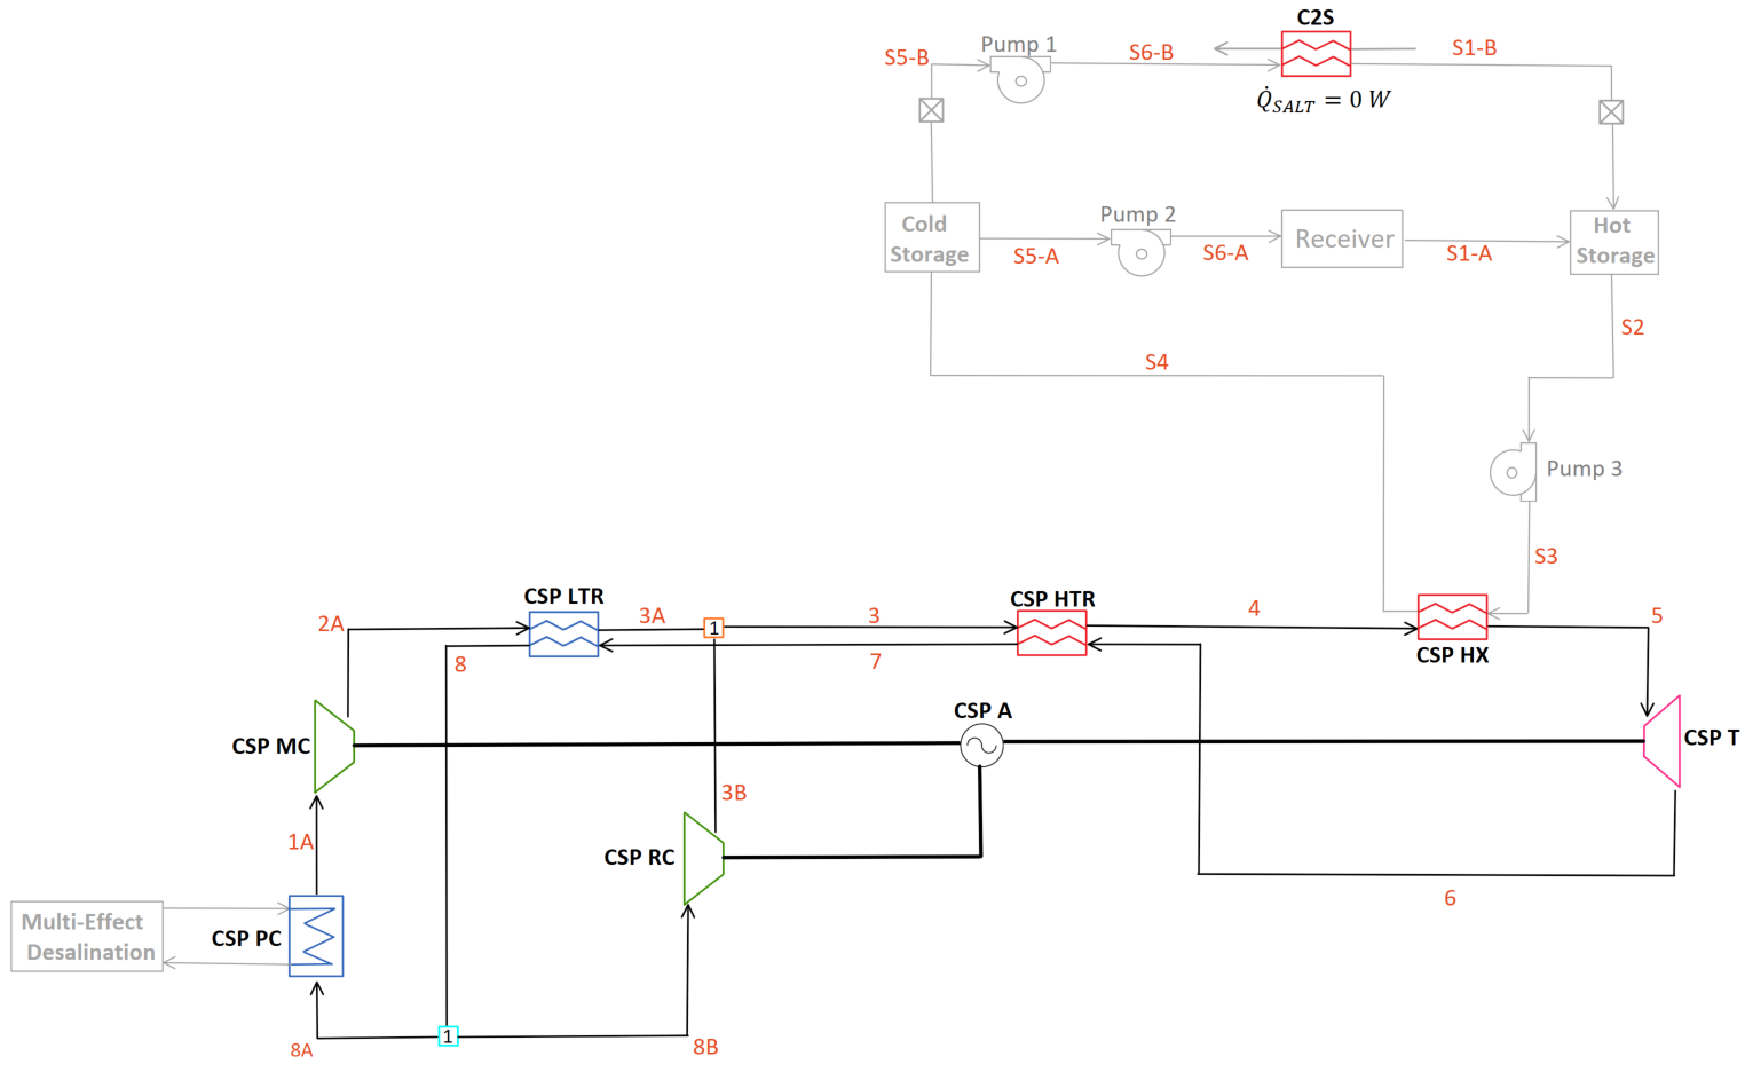
\includegraphics[width=\linewidth]{Definitions/c-csp-on.pdf}
    \caption{Diagram for C-CSP-ON with focus on electricity generation\label{c-csp-on}}
\end{figure}
\begin{paracol}{2}
\linenumbers
\switchcolumn

 Due to the individual operation while the cycles are generating electricity, C-CSP-ON is not directly impacted by the LFR low end temperatures. Instead, a sensitivity study is done on the temperature of the cold TES. Two temperatures are tested, $390^{\circ}$C and $440^{\circ}$C, to observe the impact of cold TES temperature on cycle efficiency. 


\subsubsection{C-1HTR1T-ON} 
%--------------------------------------------------------------------------------------

One drawback of having a two-cycle design, as seen in the C-LFR-ON and C-CSP-ON, is doubling the number of system components. Combining the two cycles into one would reduce redundancy and complexity. Heat addition from the CSP HX and LFR HX in parallel orientation is therefore studied in the C-1HTR1T-ON model. This model studies what impact mixing different temperature flows prior to the turbine has on cycle efficiency. The diagram for this cycle is illustrated in Figure \ref{c-1htr1t-on}.

%%\bl{be clear that Salt HX links back into the sCO2 cycle (e.g. parallel to 5-6) but is not shown to simplify the diagram. Otherwise people will wonder where it is coming from}
%\mw{After lots of tinkering, I've not solved how to get the figures to avoid spilling over the edge of the page. I think it's a problem with the MDPI template. The figures have a lot of whitespace between components and numbers, and you may need to try to compress some of them down to make them more compact.-BW}
\end{paracol}

\begin{figure}[H] 
    \widefigure
    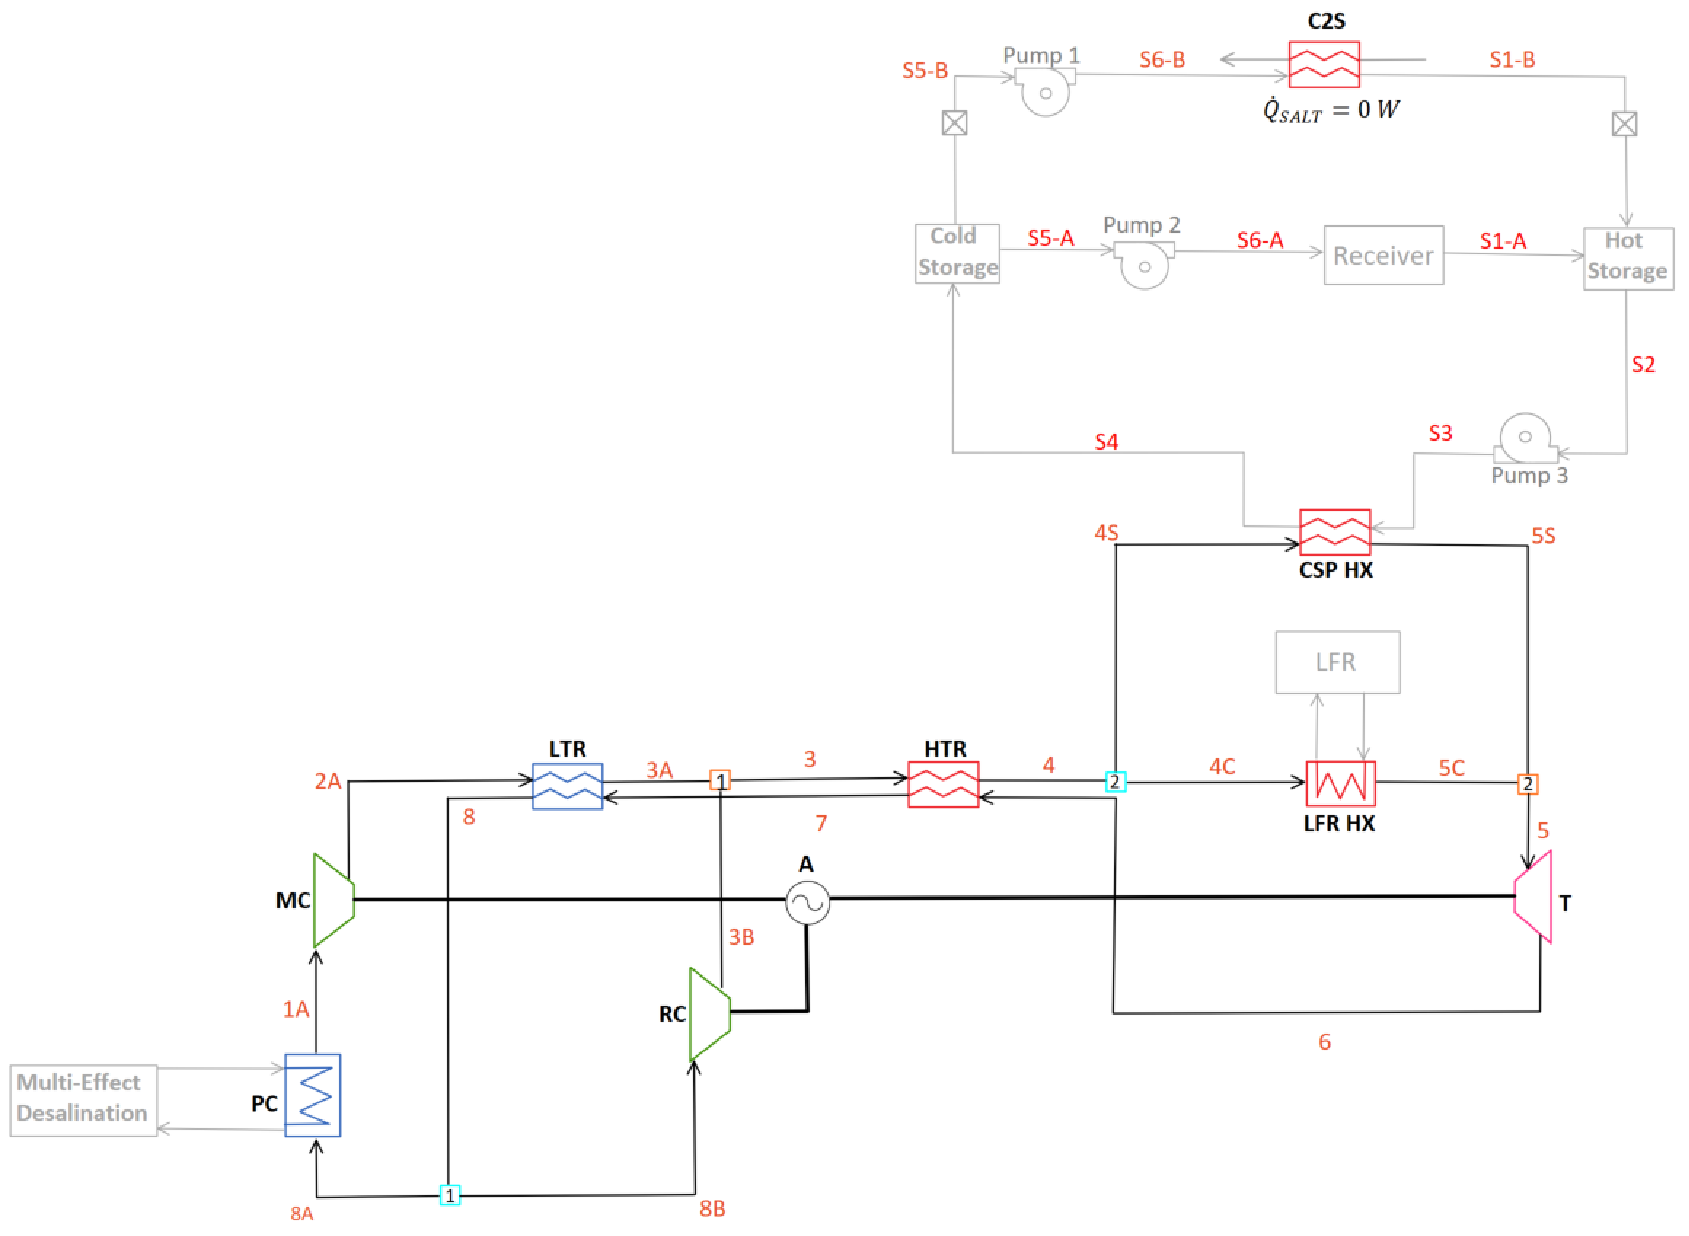
\includegraphics[width=\linewidth]{Definitions/c-1htr1t-on.pdf}
    \caption{Diagram for C-1HTR1T-ON with focus on electricity generation\label{c-1htr1t-on}}
\end{figure}


\begin{paracol}{2}
\linenumbers
\switchcolumn

The C2S is located around the turbine and LFR at state points 5 to 6 depending on the charging cycle configuration: pre, parallel, post or circulator. In the C-1HTR1T-ON cycle, the LFR HX and CSP HX have identical inlet temperatures due to splitting the flow prior to their parallel orientation. Therefore, three sensitivity studies are done on the model. The initial two studies have the low LFR temperature constrained to the value of $400^{\circ}$C with varied cold CSP TES temperature and maximized cycle efficiency. To achieve a maximum cycle efficiency, the split fraction amount of flow to the main compressor, $y_{1}$, is parametrically studied.
%\mw{State what variable(s) are manipulated in order to maximize cycle efficiency -BW} 
Two cold TES temperatures are tested with constrained LFR low temperature of $400^{\circ}$C: 
\begin{itemize}
    \item	$410^{\circ}$C: Lowest cold TES temperature possible due to the sCO$_2$ cold inlet constrained from the LFR to $400^{\circ}$C and the addition of $10^{\circ}$C approach temperature;
    \item	$440^{\circ}$C: Upper bound temperature on cold TES storage;
\end{itemize}

Additionally a third test is conducted with the desired cold TES temperature of $390^{\circ}$C and the LFR low temperature unconstrained:

\begin{itemize}
    \item	$390^{\circ}$C: Unconstrained LFR cold inlet temperature allows for the desired cold TES to be achieved;
\end{itemize}

In the third case the constraint on the LFR low temperature is removed, dropping the temperature of the LFR inlet to $380^{\circ}$C. The desired cold TES temperature of $390^{\circ}$C allows for a larger temperature drop across the CSP HX increasing dispatchability.
%%\bl{I think I understand what you're talking about but the above para could spell out all the sensitivity cases a bit more clearly, perhaps as bullets. Asp you will want to explain the criteria that go into cold storage temp. Lower = more delta T = more dispatchability -BW}


\subsubsection{C-2HTR3T-ON} 
%--------------------------------------------------------------------------------------

Mixing two different temperature flows before the turbine in a Brayton cycle has a negative effect on cycle efficiency \mw{compared to...?}. To quantify the reduction in cycle efficiency, another cycle with no mixing prior to the turbine is desired. This cycle, C-2HTR3T-ON, can be seen in Figure \ref{c-2htr3t-on} and has two high temperature recuperators and three turbines. The LFR is powering one turbine, T1, and transferring unused heat to the flow entering LFR HX through a dedicated high temperature recuperator, \hl{HTR1}. 
%\mw{The LFR doesn't recuperate heat. Clarify what you mean here. -BW} 
The cycle with heat addition from the CSP also contains two separate turbines, T2, while having a dedicated high temperature recuperator, HTR2. 
\mw{Need to explain how T2 is actually 2 separate turbines represented diagramatically as 1, and why we can model it this way.} 
After the high temperature recuperators, the two flows are combined and sent to the LTR hot side. 
%\bl{this is more about having a compromise option of intermediate complexity and efficiency}

\end{paracol}
\begin{figure}[H]
    \widefigure
    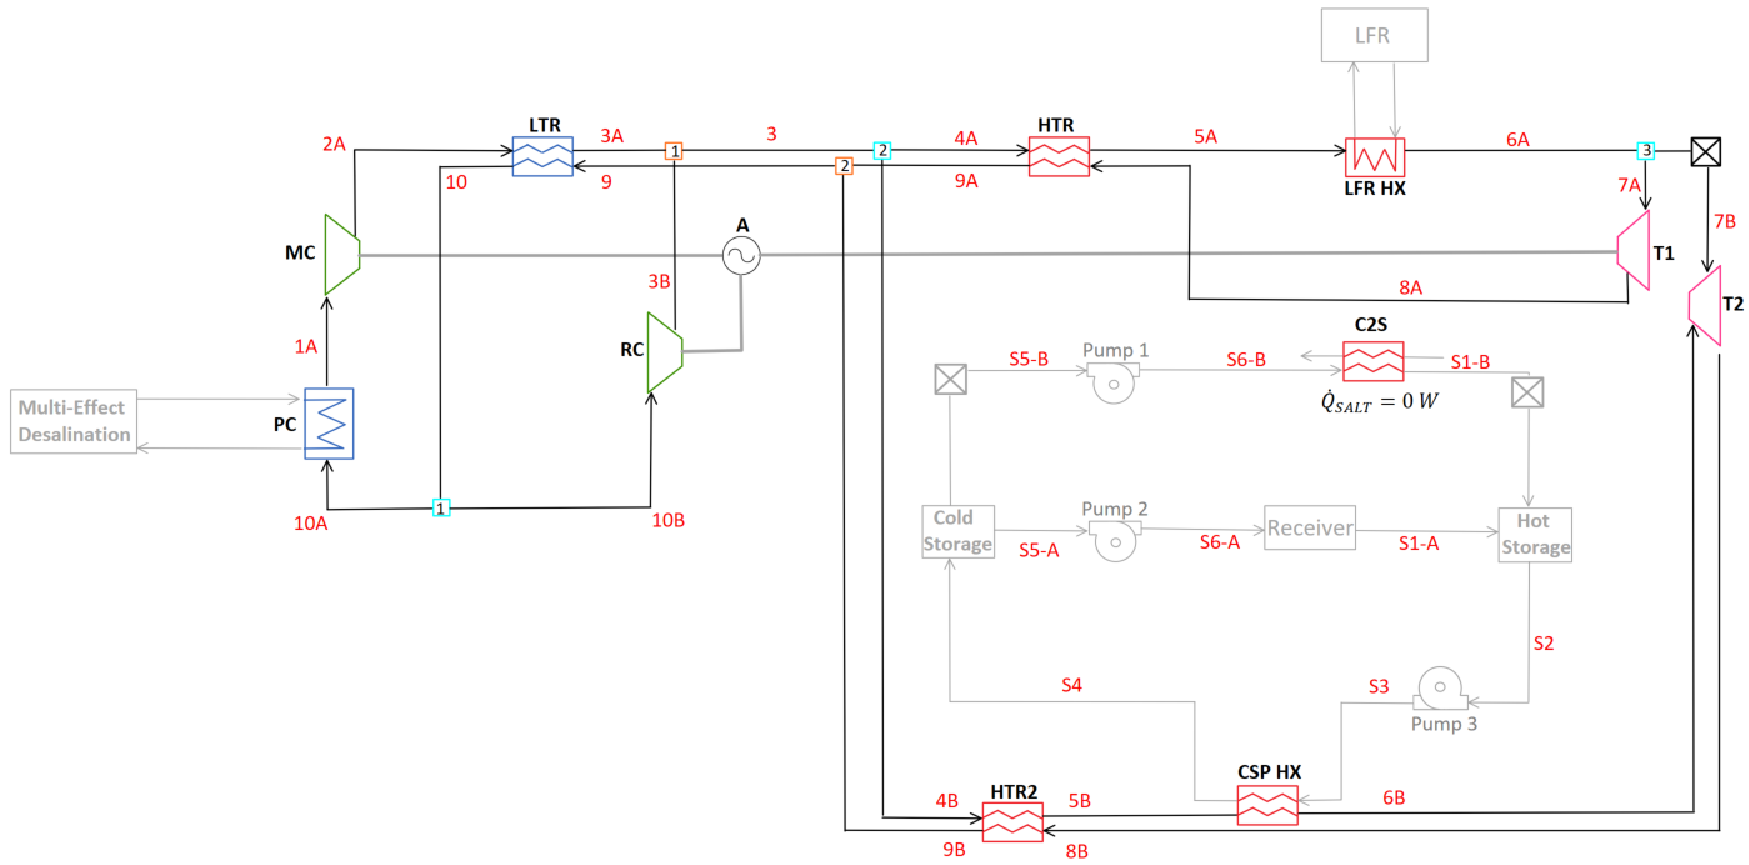
\includegraphics[width=\linewidth]{Definitions/c-2htr3t-on.pdf}
    \caption{Diagram for C-2HTR3T-ON with focus on electricity generation\label{c-2htr3t-on}}
\end{figure}
\begin{paracol}{2}
\linenumbers
\switchcolumn

The C2S heat exchanger is located around the turbine and LFR at 7A to 8A depending on the charging configuration: pre, post, parallel or circulator. Three sensitivity studies are done on the C-2HTR3T-ON model -- two with the LFR low temperature constrained and one without this constraint. The two constrained studies have varied cold CSP TES temperature with the lowest temperature of $390^{\circ}$C and highest temperature of $440^{\circ}$C. The unconstrained low LFR inlet study is calculated at a cold CSP TES temperature of $390^{\circ}$C.  
%\bl{this is clearer than the previous one but bullets could still be useful}



\subsection{Thermal Energy Storage Charging Techniques} 
%======================================================================================

Charging cycle configurations accommodate energy storage modes of operation. These configurations examine the location of LFR heat extraction via C2S. To maximize the available heat for extraction, alternator net power is set to zero, therefore requiring the turbine power to balance with the compressors' demand. Despite the components being non-ideal and consuming power, the recompression cycle continues to operate, ensuring that there is mass flow to transfer heat from the Brayton cycle to C2S. The excess energy from the LFR is thermally stored in the TES for later use when grid demand increases. Comparison of the heat extraction point in the cycle, C2S, is accomplished by implementing C2S in different locations around the turbine in the C-LFR-ON non-charging cycle configuration; C-LFR-PRE has the turbine prior to C2S, C-LFR-POST has the turbine after C2S, C-LFR-PAR has the turbine in parallel to C2S, and C-LFR-CIRC uses a circulating loop instead of in-flow implementation. C-LFR-ON is the configuration used for these studies because during charging operation, flow through the CSP HX is deactivated, effectively making all non-charging cycles take the identical form of C-LFR-ON. To quantify the effectiveness of TES charging techniques, Equation \ref{eq-eta-heatstorage} defines the heat storage efficiency, $\eta_{heatstorage}$.  
%%\bl{explain that as a (re)compression cycle is still being run for the LFR and the components are not perfectly efficient, it will consume power moving the fluid around that needs to be balanced with some of the thermal output -BW}

\begin{equation}
    \label{eq-eta-heatstorage}
    \eta_{heatstorage} = \frac{\dot{Q}_{C2S}}{\dot{Q}_{LFRHX}+\dot{Q}_{CSPHX}},
\end{equation}

In the heat storage efficiency equation, $\dot{Q}_{C2S}$ is the amount of heat transferred through C2S, and the addition of $\dot{Q}_{LFRHX}$ and $\dot{Q}_{CSPHX}$ is the total amount of heat input into the system from the LFR HX and CSP HX. 
%\mw{not a full sentence -BW}

\subsubsection{C-LFR-PRE} 
%--------------------------------------------------------------------------------------

Flow leaving the turbine contains excess thermal energy that is not transformed into electrical energy. This excess thermal energy is stored in the hot CSP TES. The diagram outlining this process is C-LFR-PRE in Fig. \ref{c-lfr-pre}. 

\mw{Careful here. Be precise about what ``excess'' means in this context. Any fluid above absolute zero technically has excess thermal energy if the reference is zero. Depending on this definition, not all excess energy from the turbine is stored in TES.} 
\mw{explain in a bit more detail what is happening that makes this configuration different from prior iterations.}

\end{paracol}
\begin{figure}[H]
    \widefigure
    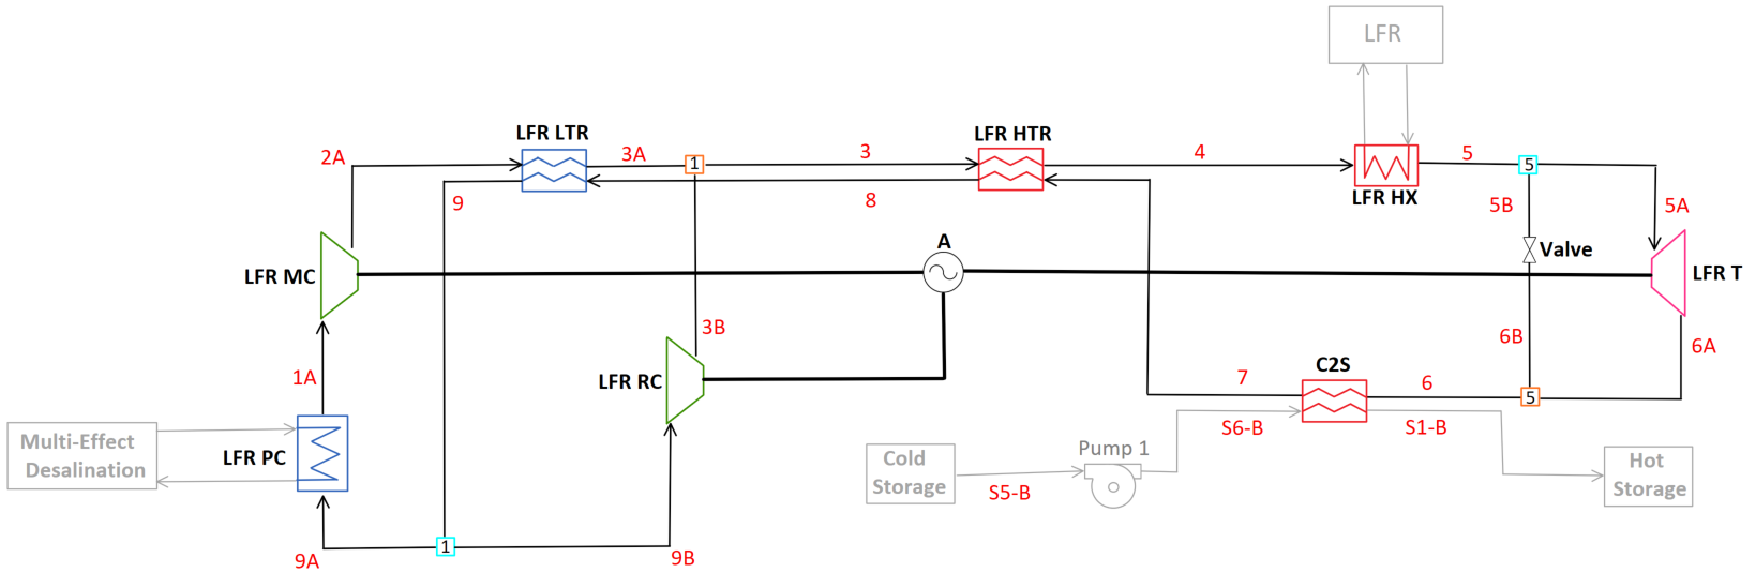
\includegraphics[width=\linewidth]{Definitions/c-lfr-pre.pdf}
    \caption{Diagram for C-LFR-PRE thermal energy storage charging orientation\label{c-lfr-pre}}
\end{figure}
\begin{paracol}{2}
\linenumbers
\switchcolumn

Problems arise with this salt charging configuration. The temperature out of the turbine is not high enough to charge the hot CSP TES to the required value of $595^{\circ}$C. To raise the temperature, some of the high temperature flow before the turbine is redirected through a valve and combined after the turbine. Combining different temperature flows and reducing the flow through the turbine has a large impact on heat storage efficiency. 



\subsubsection{C-LFR-POST} 
%--------------------------------------------------------------------------------------

Moving the heat extraction prior to the turbine is analyzed in C-LFR-POST. This diagram is seen in Figure \ref{c-lfr-post}.

\end{paracol}
\begin{figure}[H]
    \widefigure
    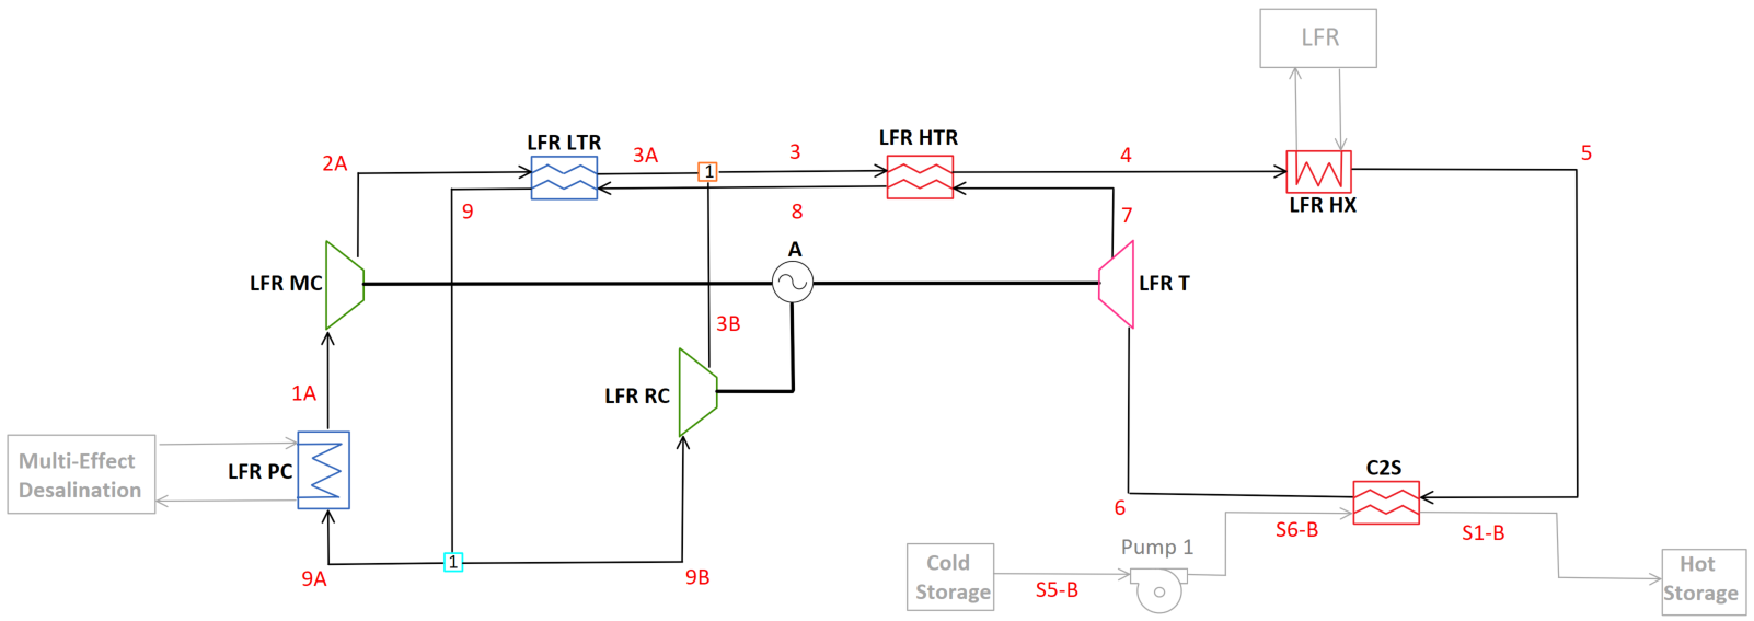
\includegraphics[width=\linewidth]{Definitions/c-lfr-post.pdf}
    \caption{Diagram for C-LFR-POST thermal energy storage charging orientation\label{c-lfr-post}}
\end{figure}
\begin{paracol}{2}
\linenumbers
\switchcolumn

This TES charging cycle extracts heat before the turbine and therefore has a large negative effect on the amount of work that the turbine is producing. The turbine power offsets the requirements of both compressors, requiring the turbine inlet temperature to be high. The amount of energy that is extracted before the turbine is small and therefore the heat storage efficiency is fractional compared to other charging techniques. There is no quantitative study done on this case because, due to the efficiency losses, it is non-viable. 

%\mw{write matter-of-factly, not in a hypothetical tense.-BW}

\subsubsection{C-LFR-PAR} 
%--------------------------------------------------------------------------------------

The requirements of the turbine and CSP hot TES can be satisfied by splitting the flow before the turbine. The flow through the salt heat exchanger in this cycle is therefore separate from the turbine. After the salt heat exchanger, a valve is needed to reduce the pressure, this TES charging cycle is C-LFR-PAR shown in Figure \ref{c-lfr-par}.

\end{paracol}
\begin{figure}[H]
    \widefigure
    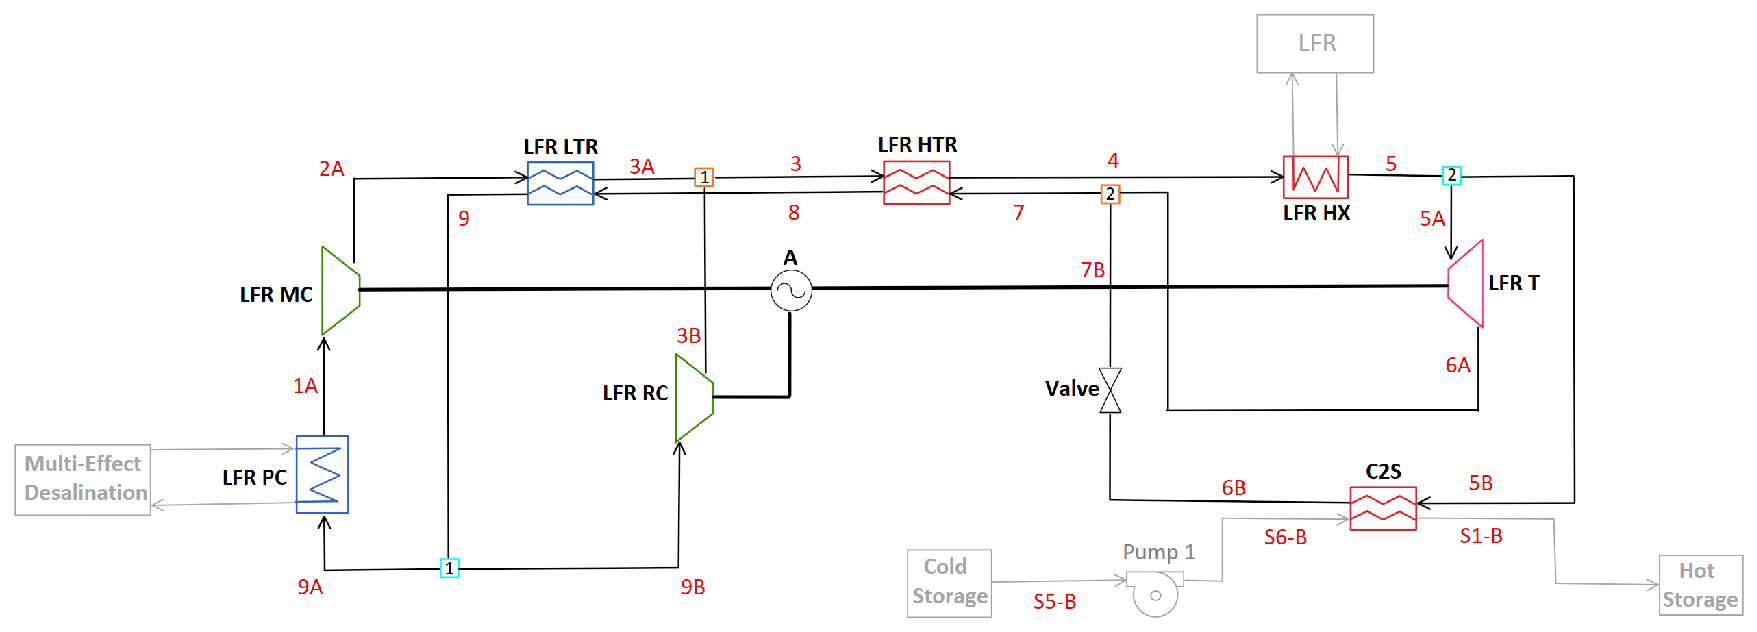
\includegraphics[width=\linewidth]{Definitions/c-lfr-par.pdf}
    \caption{Diagram for C-LFR-PAR thermal energy storage charging orientation\label{c-lfr-par}}
\end{figure}
\begin{paracol}{2}
\linenumbers
\switchcolumn

Two sensitivity studies \mw{this is one study with two parameter values, right?} with varying cold CSP TES temperature are carried out to determine the impact on heat storage efficiency. The study considers two temperature values of $390^{\circ}$C and $440^{\circ}$C.

\subsubsection{C-LFR-CIRC} 
%--------------------------------------------------------------------------------------

The full diagram for C-LFR-CIRC is shown in Figure \ref{c-lfr-circ}.

\end{paracol}
\begin{figure}[H]
    \widefigure
    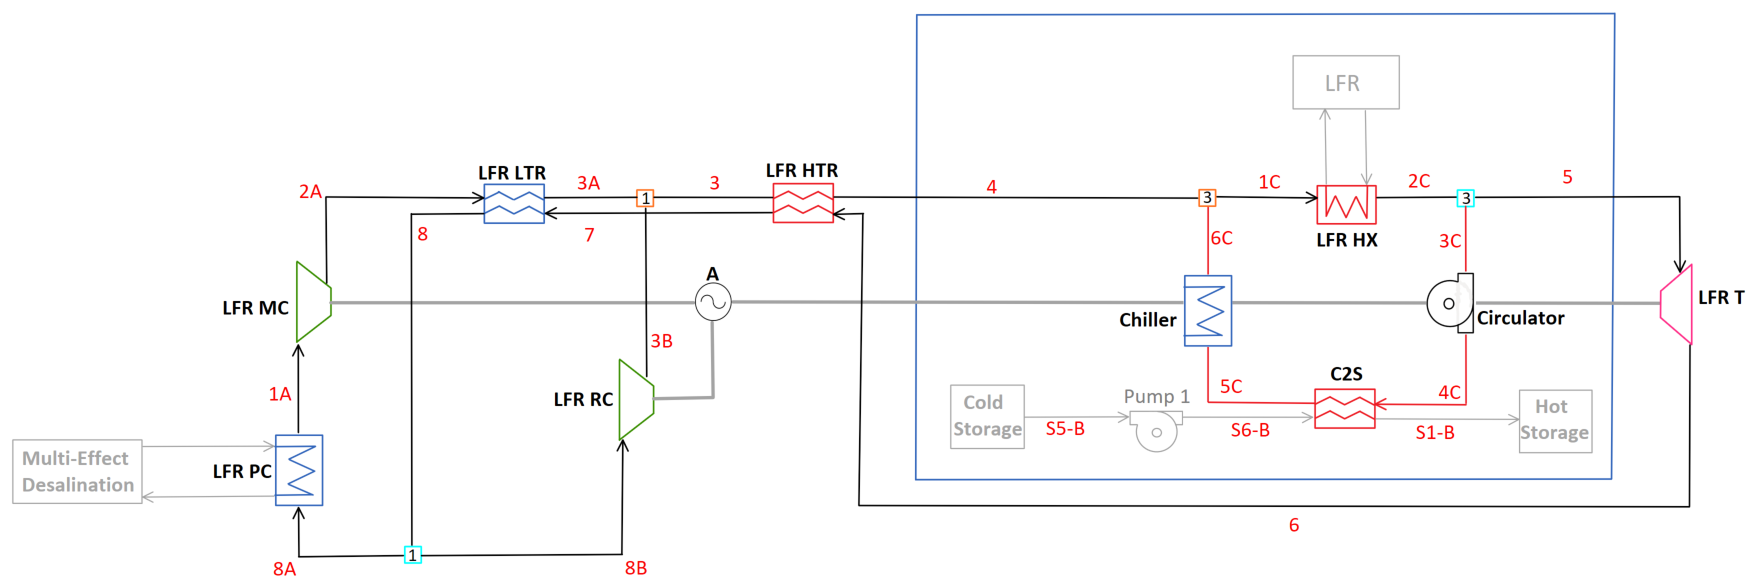
\includegraphics[width=\linewidth]{Definitions/c-lfr-circ.pdf}
    \caption{Full diagram for C-LFR-CIRC thermal energy storage charging orientation\label{c-lfr-circ}}
\end{figure}
\begin{paracol}{2}
\linenumbers
\switchcolumn

The charging subsection of this diagram is composed of a circulation cycle that has heat inputted through the LFR heat exchanger. A separated circulation cycle has a loop which avoids the losses associated with compressor and turbine, therefore achieving higher heat storage efficiency than possible with full cycle operation. This subsection is encircled in blue and can be seen in Figure \ref{c-lfr-circ-sub}.

%%\bl{explain why you are considering this case (avoid losing useful energy in compressor and turbine inefficiencies)} \mw{agree with Ben. Additional motivation is needed -BW}

\end{paracol}
\begin{figure}[H]
    \widefigure
    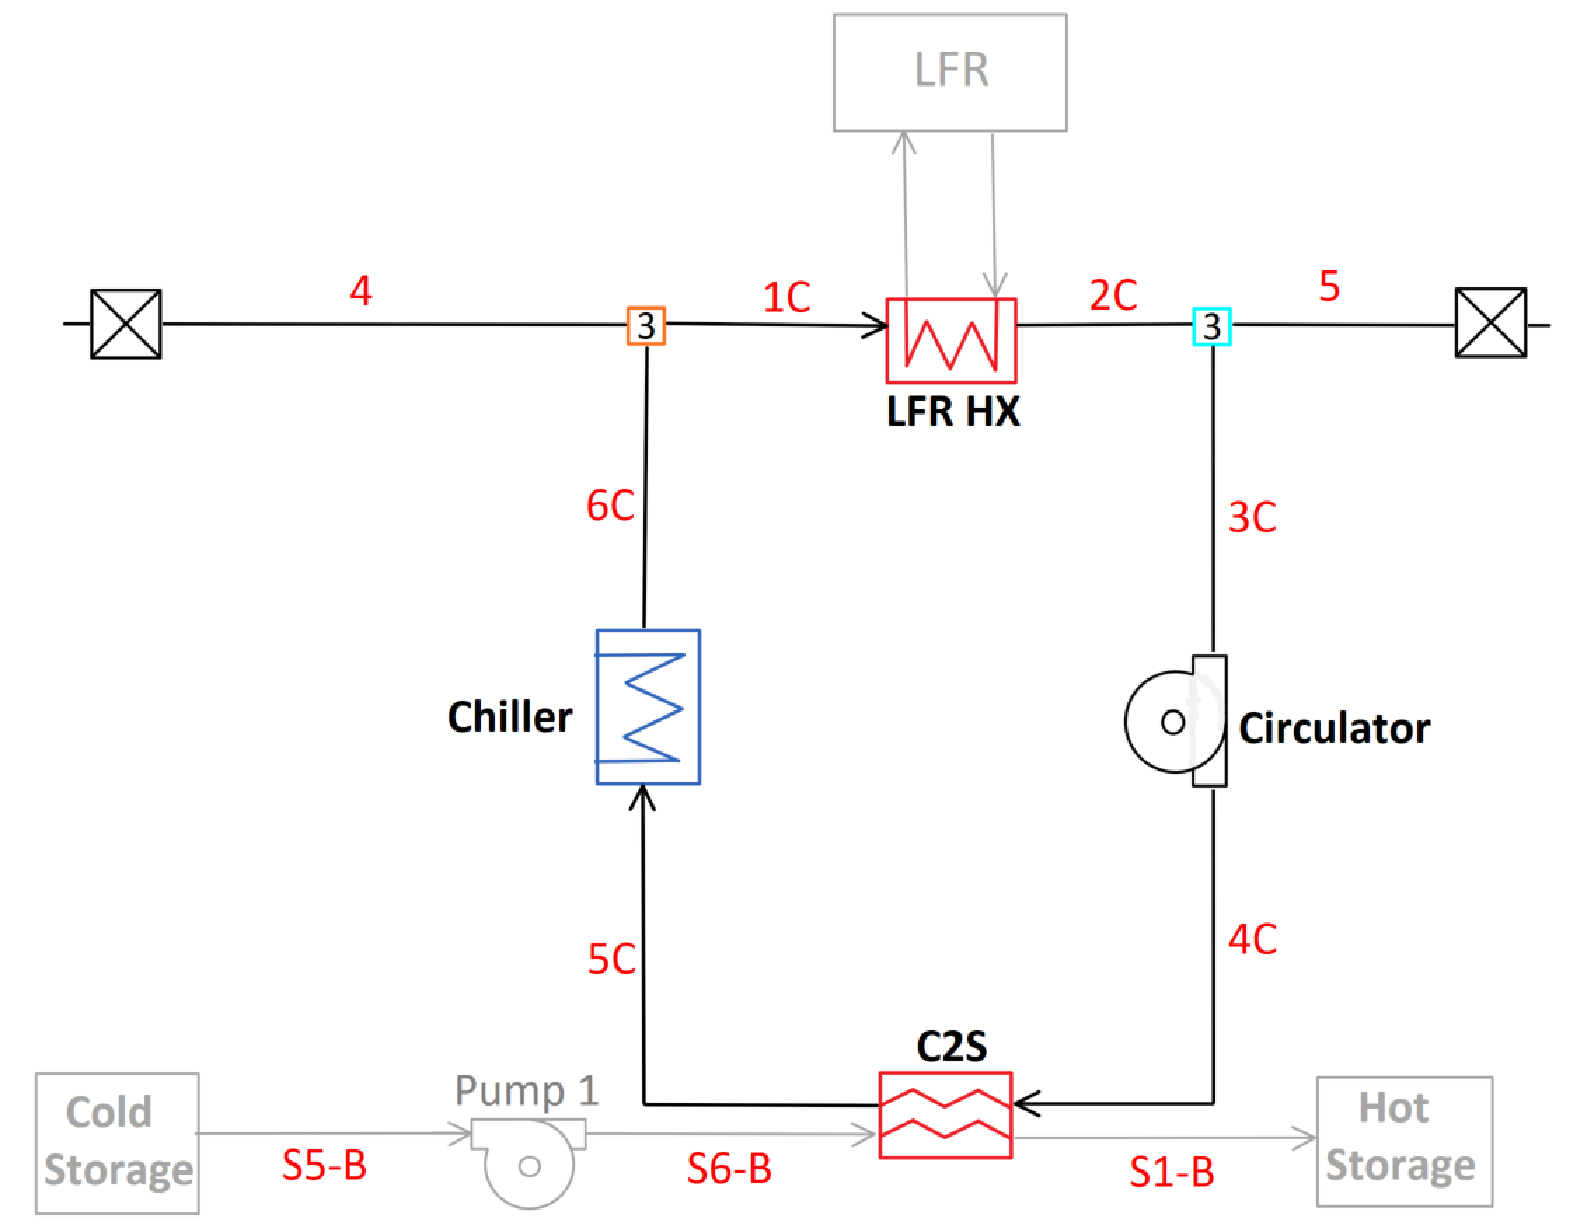
\includegraphics[width=8 cm]{Definitions/c-lfr-circ-sub.pdf}
    \caption{Diagram for C-LFR-CIRC sub-cycle thermal energy storage charging orientation\label{c-lfr-circ-sub}}
\end{figure}
\begin{paracol}{2}
\linenumbers
\switchcolumn

The flow continues through a circulator which is assumed to have negligible pressure rise (i.e. there is assumed to be negligible pressure drop in this case). A heat exchanger, C2S, extracts heat from the flow, storing the thermal energy in the hot TES for later use. Excess heat that is not extracted is then dumped into a reservoir through the chiller to bring the temperature of the flow down to LFR cool side operating temperature of $400^{\circ}$C. Three different cold TES temperatures; $390^{\circ}$C, $410^{\circ}$C, and $440^{\circ}$C, are compared in a sensitivity study. 



%%%%%%%%%%%%%%%%%%%%%%%%%%%%%%%%%%%%%%%%%%%%%%%%%%%%%%%%%%%%%%%%%%%%%%%%%%%%%%%%%%%%%%%
\section{Results and Discussion}

For all cycle configurations presented, with constrained or unconstrained LFR low temperature inlet and varied cold TES temperature, cycle and heat storage efficiencies are maximized using parametric studies on flow splitter fractions. These results are obtained using standardized values found in Table \ref{tab-cycle_sum} for a more direct comparison between cycles. Presentation and discussion of the results is fulfilled in the following section. 

\subsection{Non-Charging Cycle Configurations}
%======================================================================================

The values for the three non-charging cycle models with a focus on electrical generation, 2-cycle configuration composed of C-LFR-ON and C-CSP-ON, C-1HTR1T-ON, and C-2HTR3T-ON, are displayed in Table \ref{tab-noncharg}. 

\end{paracol}
\begin{specialtable}[H] 
    %[htbp]
    \caption{Calculated system parameters for non-charging cycle configurations with constrained (\textit{C}) and unconstrained (\textit{U}) lead-cooled fast reactor low-end temperature.\label{tab-noncharg}}
    \resizebox{\columnwidth}{!}{
    \begin{tabular}{lccccccccccc}
    \toprule
     &  & \textbf{C-LFR-ON} & & \textbf{C-CSP-ON} &  &	\textbf{C-1HTR1T-ON} &	&	&	\textbf{C-2HTR3T-ON}	&	& \\
    \textbf{Definition} & \textbf{Variable} & \textit{U} & \textit{C} & \textit{N/A} & \textit{N/A} &	\textit{U}	&	\textit{C}	&	\textit{C}	&	\textit{U}	&	\textit{C}	&	\textit{C}
    \\
    \midrule
    Cycle Efficiency (\%)	&	$\eta_{cycle}$	&	47.08	&	45.28	&	45.58	&	45.93	&	44.9	&	44.22	&	44.22	&	46.10	&	44.34	&	44.35	\\
    LFR Inlet Temperature ($^{\circ}$C)	&	$T_{4,4C,5A}$	&	415.1	&	400	&	N/A	&	N/A	&	380	&	400	&	400	&	415.2	&	400	&	400	\\
    Cold TES Temperature ($^{\circ}$C)	&	$T_{CS}$	&	N/A	&	N/A	&	390	&	440	&	390	&	410	&	440	&	390	&	390	&	440	\\
    Alternator Power (MW)	&	$\dot{W}_{A}$	&	447.3	&	430.2	&	339.1	&	340.6	&	763.9	&	752.3	&	752.6	&	783.7	&	753.7	&	754	\\
    PC Heat Transfer (MW)	&	$\dot{Q}_{PC}$	&	502.7	&	519.8	&	418.5	&	420.2	&	937.4	&	949.2	&	949.3	&	917.6	&	947.6	&	947.9	\\
    MC Power (MW)	&	$\dot{W}_{MC}$	&	115	&	118.9	&	95.73	&	96.13	&	214.5	&	194.8	&	194.8	&	209.9	&	216.8	&	216.9	\\
    RC Power (MW)	&	$\dot{W}_{RC}$	&	116.6	&	77.3	&	97.22	&	97.71	&	217.4	&	285.7	&	285.7	&	213.5	&	140.8	&	140.8	\\
    T1 Power (MW)	&	$\dot{W}_{T1}$	&	678.9	&	626.4	&	532.1	&	534.5	&	1196	&	1233	&	1233	&	679.3	&	626.3	&	626.3	\\
    T2 Power (MW)	&	$\dot{W}_{T2}$	&	N/A	&	N/A	&	N/A	&	N/A	&	N/A	&	N/A	&	N/A	&	527.8	&	485	&	485.4	\\
    MC Mass Flow Fraction (-)	&	$y_{1}$	&	0.7	&	0.7844	&	0.6996	&	0.6994	&	0.7	&	0.6333	&	0.6333	&	0.6993	&	0.7846	&	0.7846	\\
    LFR Mass Flow Fraction (-)	&	$y_{2}$	&	N/A	&	N/A	&	N/A	&	N/A	&	0.4485	&	0.4928	&	0.4929	&	0.5478	&	0.5486	&	0.5484	\\
    LTR UA Value (MW/$^{\circ}$C)	&	$UA_{LTR}$	&	54.68	&	22.84	&	45.4	&	45.53	&	102	&	91.63	&	91.64	&	134.4	&	41.56	&	41.57	\\
    LTR Capacitance Ratio (-)	&	$CR_{LTR}$	&	0.9867	&	0.8473	&	0.9858	&	0.9854	&	0.9867	&	0.9066	&	0.9066	&	0.9853	&	0.847	&	0.847	\\
    LTR Heat Transfer Rate (MW)	&	$\dot{Q}_{LTR}$	&	656.8	&	366.5	&	548.3	&	551.4	&	549.2	&	614.9	&	615.1	&	1204	&	667.1	&	667.3	\\
    LTR Effectiveness (-)	&	$\varepsilon_{LTR}$	&	0.92	&	0.8742	&	0.9201	&	0.9202	&	0.92	&	0.9485	&	0.9485	&	0.9414	&	0.8741	&	0.8741	\\
    HTR UA Value (MW/$^{\circ}$C)	&	$UA_{HTR}$	&	48.29	&	42.71	&	34.58	&	34.72	&	78.22	&	82.3	&	82.34	&	48.32	&	42.69	&	42.69	\\
    HTR Capacitance Ratio (-)	&	$CR_{HTR}$	&	0.8657	&	0.8143	&	0.8593	&	0.8594	&	0.8595	&	0.8754	&	0.8755	&	0.8661	&	0.8142	&	0.8142	\\
    HTR Heat Transfer Rate (MW)	&	$\dot{Q}_{HTR}$	&	998.1	&	1161	&	665.4	&	667.7	&	679.2	&	742.6	&	743	&	545.7	&	636.8	&	636.6	\\
    HTR Effectiveness (-)	&	$\varepsilon_{HTR}$	&	0.9544	&	0.9627	&	0.9436	&	0.9436	&	0.9445	&	0.9441	&	0.9441	&	0.9542	&	0.9627	&	0.9627	\\
    HTR2 UA Value (MW/$^{\circ}$C)	&	$UA_{HTR2}$	&	N/A	&	N/A	&	N/A	&	N/A	&	N/A	&	N/A	&	N/A	&	34.29	&	31.61	&	31.63	\\
    HTR2 Capacitance Ratio (-)	&	$CR_{HTR2}$	&	N/A	&	N/A	&	N/A	&	N/A	&	N/A	&	N/A	&	N/A	&	0.8594	&	0.8074	&	0.8074	\\
    HTR2 Heat Transfer Rate (MW)	&	$\dot{Q}_{HTR2}$	&	N/A	&	N/A	&	N/A	&	N/A	&	N/A	&	N/A	&	N/A	&	298.1	&	363.4	&	363.8	\\
    HTR2 Effectiveness (-)	&	$\varepsilon_{HTR2}$	&	N/A	&	N/A	&	N/A	&	N/A	&	N/A	&	N/A	&	N/A	&	0.9436	&	0.9561	&	0.9561	\\
    CSPHX UA Value (MW/$^{\circ}$C)	&	$UA_{CSPHX}$	&	N/A	&	N/A	&	71.34	&	26.92	&	33.72	&	73.4	&	35.05	&	70.88	&	44.92	&	23.13	\\
    CSPHX Capacitance Ratio (-)	&	$CR_{CSPHX}$	&	N/A	&	N/A	&	0.9924	&	0.701	&	0.8104	&	0.9957	&	0.8034	&	0.9926	&	0.9138	&	0.6454	\\
    CSPHX Heat Transfer Rate (MW)	&	$\dot{Q}_{CSPHX}$	&	N/A	&	N/A	&	757.6	&	760.8	&	751.3	&	751.5	&	751.9	&	751.3	&	751.3	&	751.9	\\
    CSPHX Effectiveness (-)	&	$\varepsilon_{CSPHX}$	&	N/A	&	N/A	&	0.945	&	0.945	&	0.945	&	0.9381	&	0.9374	&	0.9450	&	0.9493	&	0.9493	\\
    \bottomrule
    \end{tabular}
    }
\end{specialtable}
\begin{paracol}{2}
\linenumbers
\switchcolumn

The calculated values reported in Table \ref{tab-noncharg} are component power, mass flow fractions, and counter-flow heat exchanger specifications. Columns labeled with '$C$' headers have the LFR sCO$_2$ low inlet temperature constrained to 400$^{\circ}$C while those labeled with '$U$' are unconstrained and calculated based off of a parametric study on the MC mass flow fraction. Values listed in the Cold TES Temperature row are set to values of 390$^{\circ}$C, 410$^{\circ}$C, or 440$^{\circ}$C to study the effects that cold TES temperature has on cycle efficiency and to accommodate certain characteristics of cycle configurations. Cycles with data entries labeled not applicable (N/A) do not contain the component listed and therefore do not have values associated with the component. 

\subsubsection{Two-Cycle Configuration: C-LFR-ON and C-CSP-ON}

The two-cycle configuration has the CSP and LFR operating in separate recompression cycles when the focus is on electrical generation, therefore these two cycles are analyzed individually. C-LFR-ON has the highest efficiency during unconstrained operation with a gain of 1.8\%. The unconstrained case allows for smaller temperature gradient across the LFR, an increase in recuperator effectiveness, and an increase in recuperator capacitance ratio, all of which reduce sources of irreversibility in the cycle \cite{klein_nellis_2011}. According to studies carried out by our industry partner, Westinghouse, increasing the LFR sCO$_2$ inlet temperature above the design value of 400$^{\circ}$C has a negative effect on LFR HX outlet temperature, effectively demanding an ideal LFR heat exchanger, but does increase the LFR efficiency. Additionally, Westinghouse concluded that a lower sCO$_2$ LFR inlet temperature, down to 340$^{\circ}$C, is desirable for higher core power. The sCO$_2$ inlet temperature to the LFR increases by 15.1$^{\circ}$C to a value of 415.1$^{\circ}$C, increasing LFR efficiency but demanding a larger, more idealized, LFR heat exchanger.   
\hl{would I need more information on the LFR from westinghouse (ie report) to make these statements? additionally a conclusion to these statements needs more supporting detail, should I go with the higher efficiency or the cycle that I know works with design values?}

C-CSP-ON is not affected by constrained or unconstrained LFR sCO$_2$ inlet temperature because the two cycles are not tethered during non-charging configuration. Two individual studies are conducted on the C-CSP-ON cycle cold TES temperature, one with a lower design value of 390$^{\circ}$C and another with a higher value of 440$^{\circ}$C. A cold TES temperature of 410$^{\circ}$C is excluded since it can be presumed to have an efficiency intermediate to the 390$^{\circ}$C and 440$^{\circ}$C calculated values. Cold TES temperature is found to have a negligible effect on cycle efficiency between the two studied cases, with the 440$^{\circ}$C case gaining 0.35\%. The component that has the largest change in values is the CSP HX with a large drop in capacitance ratio and UA value, therefore the lower temperature of 390$^{\circ}$C for cold TES temperature is ideal increasing the performances of the heat exchanger. 


\subsubsection{C-1HTR1T-ON}
The single cycle configuration, C-1HTR1T-ON, has the CSP and LFR heat additions in parallel causing identical inlet conditions. Due to the 10$^{\circ}$C approach temperature, the identical inlet conditions lead to a lower bound of 410$^{\circ}$C on the cold TES temperature when the sCO$_2$ LFR inlet temperature is constrained to 400$^{\circ}$C. A supplementary 440$^{\circ}$C cold TES study is ran to test the effects that higher temperature storage has on cycle efficiency. Raising the temperature of the cold TES from 410$^{\circ}$C to 440$^{\circ}$C has no effect on cycle efficiency but did raise the solar salt mass flow rate to accommodate for the lower temperature difference across the CSP HX hot side. Increasing the solar salt mass flow rate requires more storage for the same CSP heat input, a reduction in dispatchability, and larger pumps, increasing the cost of the system. Therefore, a lower cold TES temperature is desirable. Without the constraint on the sCO$_2$ LFR inlet temperature, a study is additionally conducted with cold TES temperature set to 390$^{\circ}$C. Of these three sensitivity studies, the cycle that yielded the highest efficiency is the unconstrained, 390$^{\circ}$C cold TES with an efficiency gain of 0.68\% over the constrained cases. The high temperature difference between the hot and cold TES reduces the mass flow rate of solar salt and subsequent cost of system components. The sCO$_2$ LFR inlet temperature for the 390$^{\circ}$C cold TES study is 380$^{\circ}$C, which increases the performance of the LFR heat exchanger as well as allowing for a higher core power. 

\subsubsection{C-2HTR3T-ON}
C-2HTR3T-ON has dedicated recuperators and turbines for the LFR and CSP, allowing for independent inlet temperatures. Three studies are conducted on this cycle with two being constrained and one unconstrained sCO$_2$ LFR inlet conditions. The constrained studies have cold TES temperatures of 390$^{\circ}$C and 440$^{\circ}$, both of which have negligible efficiency differences. Similarly to the studies done on C-1HTR1T-ON, the 440$^{\circ}$C cold TES temperature case has a larger mass flow rate of solar salt and therefore increases component cost. The 390$^{\circ}$C unconstrained study has the highest efficiency with a value of 46.10\%, 1.76\% more than the constrained cases. Additionally, the sCO$_2$ LFR inlet temperature is 415.2$^{\circ}$C, 15.2$^{\circ}$C more than constrained cases, causing heat exchanger parameters to be less than ideal but increasing LFR efficiency. 

\hl{should I include in table 3 important mass flow rates like solar salt mass flow and total mass flow in sCO2?}

\subsection{Thermal Energy Storage Charging Techniques}

When the focus of the cycles is thermal storage for later use, the LFR charges the hot TES through the C2S heat exchanger. Studies done on the charging techniques, C-LFR-PRE, C-LFR-PAR, and C-LFR-CIRC, have constrained sCO$_2$ LFR inlet temperatures to 400$^{\circ}$C with set values of cold TES temperature of 390$^{\circ}$C, 410$^{\circ}$C, or 440$^{\circ}$C. The results are presented in Table \ref{tab-charg}. 

\end{paracol}
\begin{specialtable}[H] 
    %[htbp]
    \caption{Calculated system parameters for charging cycle configurations with constrained (\textit{C}) and unconstrained (\textit{U}) lead-cooled fast reactor low-end temperature.\label{tab-charg}}
    \resizebox{\columnwidth}{!}{
    \begin{tabular}{lccccccc}
    \toprule
     &  & \textbf{C-LFR-PRE} & \textbf{C-LFR-PAR} &  &	\textbf{C-LFR-CIRC} &	& \\
    \textbf{Definition} & \textbf{Variable} & \textit{C} & \textit{C} & \textit{C} & \textit{C} &	\textit{C}	&	\textit{C}\\
    \midrule
    Cold TES Temperature ($^{\circ}$C)	&	$T_{CS}$	&	390	&	390	&	440	&	390	&	410	&	440	\\
    LFR Inlet Temperature ($^{\circ}$C)	&	$T_{4,1C}$	&	400	&	400	&	400	&	400	&	400	&	400	\\
    Heat Storage Efficiency (\%)	&	$\eta_{heatstorage}$	&	34.53	&	45.30	&	45.30	&	99.92	&	89.66	&	74.29	\\
    Alternator Power (MW)	&	$\dot{W}_{A}$	&	0	&	0	&	0	&	N/A	&	N/A	&	N/A	\\
    PC Heat Transfer (MW)	&	$\dot{Q}_{PC}$	&	622	&	519.6	&	519.6	&	N/A	&	N/A	&	N/A	\\
    MC Power (MW)	&	$\dot{W}_{MC}$	&	142.3	&	118.9	&	118.9	&	N/A	&	N/A	&	N/A	\\
    RC Power (MW)	&	$\dot{W}_{RC}$	&	21.89	&	77.28	&	77.28	&	N/A	&	N/A	&	N/A	\\
    Turbine Power (MW)	&	$\dot{W}_{T}$	&	164.2	&	196.2	&	196.2	&	N/A	&	N/A	&	N/A	\\
    Chiller Heat Transfer (MW)	&	$\dot{Q}_{chill}$	&	N/A	&	N/A	&	N/A	&	0.7245	&	98.25	&	244.2	\\
    MC Mass Flow Fraction (-)	&	$y_{1}$	&	0.9389	&	0.7844	&	0.7844	&	N/A	&	N/A	&	N/A	\\
    C2S Mass Flow Fraction (-)	&	$y_{2}$	&	N/A	&	0.6867	&	0.6867	&	N/A	&	N/A	&	N/A	\\
    Valve Mass Flow Fraction (-)	&	$y_{5}$	&	0.7378	&	N/A	&	N/A	&	N/A	&	N/A	&	N/A	\\
    LTR UA Value (MW/$^{\circ}$C)	&	$UA_{LTR}$	&	6.99	&	22.83	&	22.83	&	N/A	&	N/A	&	N/A	\\
    LTR Capacitance Ratio (-)	&	$CR_{LTR}$	&	0.6754	&	0.8473	&	0.8743	&	N/A	&	N/A	&	N/A	\\
    LTR Heat Transfer Rate (MW)	&	$\dot{Q}_{LTR}$	&	93.05	&	366.4	&	366.4	&	N/A	&	N/A	&	N/A	\\
    LTR Effectiveness (-)	&	$\varepsilon_{LTR}$	&	0.6384	&	0.8742	&	0.8742	&	N/A	&	N/A	&	N/A	\\
    HTR UA Value (MW/$^{\circ}$C)	&	$UA_{HTR}$	&	41.69	&	42.69	&	42.69	&	N/A	&	N/A	&	N/A	\\
    HTR Capacitance Ratio (-)	&	$CR_{HTR}$	&	0.7531	&	0.8143	&	0.8143	&	N/A	&	N/A	&	N/A	\\
    HTR Heat Transfer Rate (MW)	&	$\dot{Q}_{HTR}$	&	1567	&	1160	&	1160	&	N/A	&	N/A	&	N/A	\\
    HTR Effectiveness (-)	&	$\varepsilon_{HTR}$	&	0.9695	&	0.9627	&	0.9627	&	N/A	&	N/A	&	N/A	\\
    C2S UA Value (MW/$^{\circ}$C)	&	$UA_{C2S}$	&	9.04	&	8.037	&	14.24	&	48.29	&	43.16	&	35.63	\\
    C2S Capacitance Ratio (-)	&	$CR_{C2S}$	&	0.4735	&	0.7556	&	0.9339	&	0.8755	&	0.8599	&	0.8294	\\
    C2S Heat Transfer Rate (MW)	&	$\dot{Q}_{C2S}$	&	328	&	430.4	&	430.4	&	949.3	&	851.8	&	705.8	\\
    C2S Effectiveness (-)	&	$\varepsilon_{C2S}$	&	0.9368	&	0.8275	&	0.8307	&	0.9511	&	0.9459	&	0.9355	\\
    C2S Approach Temperature ($^{\circ}$C)	&	$\delta_{C2S}$	&	10	&	35	&	26.27	&	10	&	10	&	10	\\
    \bottomrule
    \end{tabular}
    }
\end{specialtable}
\begin{paracol}{2}
\linenumbers
\switchcolumn

\subsubsection{C-LFR-PRE}
The TES charging technique with the turbine prior to the C2S heat exchanger, C-LFR-PRE, requires the temperature of the C2S inlet to be high enough to charge the hot TES. The hot TES is at a temperature of 560$^{\circ}$C, with a 10$^{\circ}$C approach temperature, therefore the inlet temperature to C2S is required to be at least 570$^{\circ}$C. In cases where the turbine outlet temperature is less than 570$^{\circ}$C, a isenthalpic valve bypasses flow from the high temperature turbine inlet and mixes with the low temperature turbine outlet raising the temperature prior to the C2S heat exchanger. For the C-LFR-PRE configuration to be viable, it requires a larger temperature than the set LFR HX outlet temperature of 595$^{\circ}$C. With this low of a LFR outlet temperature, 73.78\% of the flow is redirected around the turbine to raise the temperature prior to C2S. As the temperature of the hot TES is raised above a value of 540$^{\circ}$C, the amount of flow around the turbine approaches 100\% and balancing the turbine power to compressor power is infeasible. The temperature in the hot TES is therefore set to a lower value of 540$^{\circ}$C to allow for operation of this cycle. With heat storage efficiency maximized, 93.89\% of the flow is sent to the main compressor, rejecting 622 MW of heat out of the cycle through the precooler. This amount of rejected heat is reflected in a heat storage efficiency of 34.53\%, the lowest of all tested TES charging configurations.

\subsubsection{C-LFR-PAR}

To test the effects of splitting flow prior to the turbine, a parallel configuration C-LFR-PAR is studied. To reduce the pressure from 28.8 MPa to 8.8 MPa, an isenthalpic valve is required after heat is extracted for storage through C2S. With this configuration two different values for cold TES are studied, one with a cold TES storage of 390$^{\circ}$C the other with a temperature of 440$^{\circ}$C. A noteworthy difference for this cycle is the C2S approach temperature is not set to 10$^{\circ}$C. Defining the approach temperature as 10$^{\circ}$C causes the energy balance governing combiner 2 to be over constrained. Therefore this value is free and calculated to be 35$^{\circ}$C for the 390$^{\circ}$C case and 26.27$^{\circ}$C for the 440$^{\circ}$C case. Both of these different temperature cold TES studies do not change the cycle parameters because, as seen in C-1HTR1T-ON and C-2HTR3T-ON, the solar salt mass flow rate adjusts to accommodate for the temperature difference. The higher cold TES temperature of 440$^{\circ}$C causes the mass flow rate in the CSP to increase by approximately 650 kg/s. Increasing the mass flow rate has a higher demand on system components but in this situation it allows for the salt to be charged at a higher rate, increasing the storage capabilities. Both cycles have a heat storage efficiency of 45.30\%. \hl{Should I include solar salt mass flow also in table 4?}

\subsubsection{C-LFR-CIRC}

C-LFR-CIRC is a thermal energy storage charging technique which does not suffer from losses associated with turbines, compressors, and heat exchangers. This is due to the fact that a separate recirculation cycle is modeled taking heat directly from the LFR, passing it through a recirculating pump, exchanges the heat into the hot TES through C2S, then removes heat in a chiller to bring the temperature of the flow down to the inlet temperature of the LFR, 400$^{\circ}$C. This is the most adoptable TES charging technique a wide range of possible TES charging temperatures with almost all of the heat from the LFR being transferred into the hot TES depending on the temperature. Multiple temperatures for the cold TES are studied; 390$^{\circ}$C, 410$^{\circ}$C, and 440$^{\circ}$C. Of these three temperatures, the highest efficiency is a cold TES temperature of 390$^{\circ}$ with a heat storage efficiency of 99.92\%. The heat storage efficiency reduces as the temperature of the cold TES is increased, the 410$^{\circ}$C case has an efficiency of 89.66\% while the 440$^{\circ}$C case has an efficiency of 74.29\%. This reduction in efficiency is due to the inlet temperature condition on the LFR, the higher the temperature of the cold TES the higher the temperature of the C2S outlet and therefore the more heat is being extracted through the chiller to bring the flow temperature down to the LFR inlet temperature. A drawback of this TES charging technique is the additional components needed for the circulation loop, with an additional chiller and circulator component, adding cost. 

%%%%%%%%%%%%%%%%%%%%%%%%%%%%%%%%%%%%%%%%%%%%%%%%%%%%%%%%%%%%%%%%%%%%%%%%%%%%%%%%%%%%%%%
\section{Conclusions}

% This section is not mandatory, but can be added to the manuscript if the discussion is unusually long or complex.

\end{paracol}




% \subsection{Small Tables}
% %--------------------------------------------------------------------------------------

% Modeling the C-LFR-ON cycle in EES yielded the results in Table \ref{tab-c-lfr-on}. 

% \begin{specialtable}[H] 
%     %[htbp]
%     \caption{Calculated system parameters for non-charging C-LFR-ON cycle configuration with constrained (\textit{C}) and unconstrained (\textit{U}) lead-cooled fast reactor low-end temperature.\label{tab-c-lfr-on}}
%     \begin{tabular}{lccc}
%     \toprule
%     \textbf{Definition} & \textbf{Variable} & \textit{U} & \textit{C}\\
%     \midrule
%     LFR Inlet Temperature ($^{\circ}$C)	&	$T_{4}$	&	395.1	&	400	\\
%     Cycle Efficiency (\%)	&	$\eta_{cycle}$	&	47.08	&	45.28	\\
%     Alternator Power (MW)	&	$\dot{W}_{A}$	&	447.3	&	430.2	\\
%     PC Heat Transfer (MW)	&	$\dot{Q}_{PC}$	&	502.7	&	519.8	\\
%     MC Power (MW)	&	$\dot{W}_{MC}$	&	115	&	118.9	\\
%     RC Power (MW)	&	$\dot{W}_{RC}$	&	116.6	&	77.3	\\
%     Turbine Power (MW)	&	$\dot{W}_{T}$	&	678.9	&	626.4	\\
%     MC Mass Flow Fraction (-)	&	$y_{1}$	&	0.7	&	0.7844	\\
%     LTR UA Value (MW/$^{\circ}$C)	&	$UA_{LTR}$	&	54.68	&	22.84	\\
%     LTR Capacitance Ratio (-)	&	$CR_{LTR}$	&	0.9867	&	0.8473	\\
%     LTR Heat Transfer Rate (MW)	&	$\dot{Q}_{LTR}$	&	656.8	&	366.5	\\
%     LTR Effectiveness (-)	&	$\varepsilon_{LTR}$	&	0.92	&	0.8742	\\
%     HTR UA Value (MW/$^{\circ}$C)	&	$UA_{HTR}$	&	48.29	&	42.71	\\
%     HTR Capacitance Ratio (-)	&	$CR_{HTR}$	&	0.8657	&	0.9627	\\
%     HTR Heat Transfer Rate (MW)	&	$\dot{Q}_{HTR}$	&	998.1	&	1161	\\
%     HTR Effectiveness (-)	&	$\varepsilon_{HTR}$	&	0.9544	&	0.9627	\\
%     \bottomrule
%     \end{tabular}\\
% \end{specialtable}

% \textbf{Discussion of Results}



% The EES model outputs for C-CSP-ON are listed in Table \ref{tab-c-csp-on}.

% \begin{specialtable}[H] 
%     %[htbp] 
%     \caption{Calculated system parameters for non-charging C-CSP-ON cycle configuration with varied TES cold temperature. \label{tab-c-csp-on}}
%     \begin{tabular}{lccc}
%     \toprule
%     \textbf{Definition} & \textbf{Variable} &  &\\
%     \midrule
%     Cold TES Temperature ($^{\circ}$C)	&	$T_{CS}$	&	390	&	440	\\
%     Cycle Efficiency (\%)	&	$\eta_{cycle}$	&	45.58	&	45.93	\\
%     Alternator Power (MW)	&	$\dot{W}_{A}$	&	339.1	&	340.6	\\
%     PC Heat Transfer (MW)	&	$\dot{Q}_{PC}$	&	418.5	&	420.2	\\
%     MC Power (MW)	&	$\dot{W}_{MC}$	&	95.73	&	96.13	\\
%     RC Power (MW)	&	$\dot{W}_{RC}$	&	97.22	&	97.71	\\
%     Turbine Power (MW)	&	$\dot{W}_{T}$	&	532.1	&	534.5	\\
%     MC Mass Flow Fraction (-)	&	$y_{1}$	&	0.6996	&	0.6994	\\
%     LTR UA Value (MW/$^{circ}$C)	&	$UA_{LTR}$	&	45.4	&	45.53	\\
%     LTR Capacitance Ratio (-)	&	$CR_{LTR}$	&	0.9858	&	0.9854	\\
%     LTR Heat Transfer Rate (MW)	&	$\dot{Q}_{LTR}$	&	548.3	&	551.4	\\
%     LTR Effectiveness (-)	&	$\varepsilon_{LTR}$	&	0.9201	&	0.9202	\\
%     HTR UA Value (MW/$^{\circ}$C)	&	$UA_{HTR}$	&	34.58	&	34.72	\\
%     HTR Capacitance Ratio (-)	&	$CR_{HTR}$	&	0.8593	&	0.8594	\\
%     HTR Heat Transfer Rate (MW)	&	$\dot{Q}_{HTR}$	&	665.4	&	667.7	\\
%     HTR Effectiveness (-)	&	$\varepsilon_{HTR}$	&	0.9436	&	0.9436	\\
%     CSPHX UA Value (MW/$^{\circ}$C)	&	$UA_{CSPHX}$	&	71.34	&	26.92	\\
%     CSPHX Capacitance Ratio (-)	&	$CR_{CSPHX}$	&	0.9924	&	0.701	\\
%     CSPHX Heat Transfer Rate (MW)	&	$\dot{Q}_{CSPHX}$	&	757.6	&	760.8	\\
%     CSPHX Effectiveness (-)	&	$\varepsilon_{CSPHX}$	&	0.945	&	0.945	\\
%     \bottomrule
%     \end{tabular}\\
% \end{specialtable}

% \textbf{Discussion of Results}

% %--------------------------------------------------------------------------------------

% These values are displayed in Table \ref{tab-c-1htr1t-on}.

% \begin{specialtable}[H] 
%     %[htbp] 
%     \caption{Calculated system parameters for non-charging C-1HTR1T-ON cycle configuration with constrained (\textit{C}) and unconstrained (\textit{U}) lead-cooled fast reactor low-end temperature. Temperature of TES cold temperature is also varied.\label{tab-c-1htr1t-on}}
%     \begin{tabular}{lcccc}
%     \toprule
%     \textbf{Definition} & \textbf{Variable} & \textbf{C-1HTR1T-ON}\\
%     & & \textit{U} & \textit{C} & \textit{C}\\
%     \midrule	
%     Cold TES Temperature ($^{\circ}$C)	&	$T_{CS}$	&	390	&	410	&	440	\\
%     LFR Inlet Temperature ($^{\circ}$C)	&	$T_{4C}$	&	380	&	400	&	400	\\
%     Cycle Efficiency (\%)	&	$\eta_{cycle}$	&	44.9	&	44.22	&	44.22	\\
%     Alternator Power (MW)	&	$\dot{W}_{A}$	&	763.9	&	752.3	&	752.6	\\
%     PC Heat Transfer (MW)	&	$\dot{Q}_{PC}$	&	937.4	&	949.2	&	949.3	\\
%     MC Power (MW)	&	$\dot{W}_{MC}$	&	214.5	&	194.8	&	194.8	\\
%     RC Power (MW)	&	$\dot{W}_{RC}$	&	217.4	&	285.7	&	285.7	\\
%     Turbine Power (MW)	&	$\dot{W}_{T}$	&	1196	&	1233	&	1233	\\
%     MC Mass Flow Fraction (-)	&	$y_{1}$	&	0.7	&	0.6333	&	0.6333	\\
%     LFR Mass Flow Fraction (-)	&	$y_{2}$	&	0.4485	&	0.4928	&	0.4929	\\
%     LTR UA Value (MW/$^{\circ}$C)	&	$UA_{LTR}$	&	102	&	91.63	&	91.64	\\
%     LTR Capacitance Ratio (-)	&	$CR_{LTR}$	&	0.9867	&	0.9066	&	0.9066	\\
%     LTR Heat Transfer Rate (MW)	&	$\dot{Q}_{LTR}$	&	549.2	&	614.9	&	615.1	\\
%     LTR Effectiveness (-)	&	$\varepsilon_{LTR}$	&	0.92	&	0.9485	&	0.9485	\\
%     HTR UA Value (MW/$^{\circ}$C)	&	$UA_{HTR}$	&	78.22	&	82.3	&	82.34	\\
%     HTR Capacitance Ratio (-)	&	$CR_{HTR}$	&	0.8595	&	0.8754	&	0.8755	\\
%     HTR Heat Transfer Rate (MW)	&	$\dot{Q}_{HTR}$	&	679.2	&	742.6	&	743	\\
%     HTR Effectiveness (-)	&	$\varepsilon_{HTR}$	&	0.9445	&	0.9441	&	0.9441	\\
%     CSPHX UA Value (MW/$^{\circ}$C)	&	$UA_{CSPHX}$	&	33.72	&	73.4	&	75.19	\\
%     CSPHX Capacitance Ratio (-)	&	$CR_{CSPHX}$	&	0.8104	&	0.9957	&	0.8034	\\
%     CSPHX Heat Transfer Rate (MW)	&	$\dot{Q}_{CSPHX}$	&	751.3	&	751.5	&	751.9	\\
%     CSPHX Effectiveness (-)	&	$\varepsilon_{CSPHX}$	&	0.945	&	0.9381	&	0.9374	\\
%     \bottomrule
%     \end{tabular}\\
% \end{specialtable}

% \textbf{Discussion of Results}

% %--------------------------------------------------------------------------------------

% The calculated values from these studies are displayed in Table \ref{tab-c-2htr3t-on}.

% \begin{specialtable}[H]
%     %[htbp]
%     \caption{Calculated system parameters for non-charging C-2HTR3T-ON cycle configuration with constrained (\textit{C}) and unconstrained (\textit{U}) lead-cooled fast reactor low-end temperature.\label{tab-c-2htr3t-on}}
%     \begin{tabular}{lcccc}
%     \toprule
%     \textbf{Definition} & \textbf{Variable} & \textbf{C-2HTR3T-ON} &\\
%     & & \textit{U} & \textit{C} & \textit{C}\\
%     \midrule	
%     Cold TES Temperature ($^{\circ}$C)	&	$T_{CS}$	&	390	&	390	&	440	\\
%     LFR Inlet Temperature ($^{\circ}$C)	&	$T_{5A}$	&	395.2	&	400	&	400	\\
%     Cycle Efficiency (\%)	&	$\eta_{cycle}$	&	46.10	&	44.34	&	44.35	\\
%     Alternator Power (MW)	&	$\dot{W}_{A}$	&	783.7	&	753.7	&	754	\\
%     PC Heat Transfer (MW)	&	$\dot{Q}_{PC}$	&	917.6	&	947.6	&	947.9	\\
%     MC Power (MW)	&	$\dot{W}_{MC}$	&	209.9	&	216.8	&	216.9	\\
%     RC Power (MW)	&	$\dot{W}_{RC}$	&	213.5	&	140.8	&	140.8	\\
%     T1 Power (MW)	&	$\dot{W}_{T1}$	&	679.3	&	626.3	&	626.3	\\
%     T2 Power (MW)	&	$\dot{W}_{T2}$	&	527.8	&	485	&	485.4	\\
%     MC Mass Flow Fraction (-)	&	$y_{1}$	&	0.6993	&	0.7846	&	0.7846	\\
%     LFR Mass Flow Fraction (-)	&	$y_{2}$	&	0.5478	&	0.5486	&	5.48E-01	\\
%     LTR UA Value (MW/$^{\circ}$C)	&	$UA_{LTR}$	&	134.4	&	41.56	&	41.57	\\
%     LTR Capacitance Ratio (-)	&	$CR_{LTR}$	&	0.9853	&	0.847	&	0.847	\\
%     LTR Heat Transfer Rate (MW)	&	$\dot{Q}_{LTR}$	&	1204	&	667.1	&	667.3	\\
%     LTR Effectiveness (-)	&	$\varepsilon_{LTR}$	&	0.9414	&	0.8741	&	0.8741	\\
%     HTR1 UA Value (MW/$^{\circ}$C)	&	$UA_{HTR1}$	&	48.32	&	42.69	&	42.69	\\
%     HTR1 Capacitance Ratio (-)	&	$CR_{HTR1}$	&	0.8661	&	0.8142	&	0.8142	\\
%     HTR1 Heat Transfer Rate (MW)	&	$\dot{Q}_{HTR1}$	&	545.7	&	636.8	&	636.6	\\
%     HTR1 Effectiveness (-)	&	$\varepsilon_{HTR1}$	&	0.9542	&	0.9627	&	0.9627	\\
%     HTR2 UA Value (MW/$^{\circ}$C)	&	$UA_{HTR2}$	&	34.29	&	31.61	&	31.63	\\
%     HTR2 Capacitance Ratio (-)	&	$CR_{HTR2}$	&	0.8594	&	0.8074	&	0.8074	\\
%     HTR2 Heat Transfer Rate (MW)	&	$\dot{Q}_{HTR2}$	&	298.1	&	363.4	&	363.8	\\
%     HTR2 Effectiveness (-)	&	$\varepsilon_{HTR2}$	&	0.9436	&	0.9561	&	0.9561	\\
%     CSPHX UA Value (MW/$^{\circ}$C)	&	$UA_{CSPHX}$	&	70.88	&	44.92	&	23.13	\\
%     CSPHX Capacitance Ratio (-)	&	$CR_{CSPHX}$	&	0.9926	&	0.9138	&	0.6454	\\
%     CSPHX Heat Transfer Rate (MW)	&	$\dot{Q}_{CSPHX}$	&	751.3	&	751.3	&	751.9	\\
%     CSPHX Effectiveness (-)	&	$\varepsilon_{CSPHX}$	&	0.9450	&	0.9493	&	0.9493	\\
%     \bottomrule
%     \end{tabular}\\
% \end{specialtable}

% \textbf{Discussion of Results}

% %======================================================================================

% %--------------------------------------------------------------------------------------

% The calculations from this TES charging technique are shown in Table \ref{tab-c-lfr-pre}.

% \begin{specialtable}[H]
%     %[htbp]
%     \caption{Calculated system parameters for salt charging C-LFR-PRE cycle configuration with TES cold storage set to 663.2 K.\label{tab-c-lfr-pre}}
%     \begin{tabular}{lcc}
%     \toprule
%     \textbf{Definition} & \textbf{Variable} & \textbf{C-LFR-PRE}\\
%     & & \textit{C}\\
%     \midrule	
%     Cold TES Temperature ($^{\circ}$C)	&	$T_{CS}$	&	390	\\
%     LFR Inlet Temperature ($^{\circ}$C)	&	$T_{4}$	&	400	\\
%     Heat Storage Efficiency (\%)	&	$\eta_{heatstorage}$	&	34.53	\\
%     Alternator Power (MW)	&	$\dot{W}_{A}$	&	0	\\
%     PC Heat Transfer (MW)	&	$\dot{Q}_{PC}$	&	622	\\
%     MC Power (MW)	&	$\dot{W}_{MC}$	&	142.3	\\
%     RC Power (MW)	&	$\dot{W}_{RC}$	&	21.89	\\
%     Turbine Power (MW)	&	$\dot{W}_{T}$	&	164.2	\\
%     MC Mass Flow Fraction (-)	&	$y_{1}$	&	0.9389	\\
%     Valve Mass Flow Fraction (-)	&	$y_{5}$	&	0.7378	\\
%     LTR UA Value (MW/$^{\circ}$C)	&	$UA_{LTR}$	&	0.699	\\
%     LTR Capacitance Ratio (-)	&	$CR_{LTR}$	&	0.6754	\\
%     LTR Heat Transfer Rate (MW)	&	$\dot{Q}_{LTR}$	&	93.05	\\
%     LTR Effectiveness (-)	&	$\varepsilon_{LTR}$	&	0.6384	\\
%     HTR UA Value (MW/$^{\circ}$C)	&	$UA_{HTR}$	&	41.69	\\
%     HTR Capacitance Ratio (-)	&	$CR_{HTR}$	&	0.7531	\\
%     HTR Heat Transfer Rate (MW)	&	$\dot{Q}_{HTR}$	&	1567	\\
%     HTR Effectiveness (-)	&	$\varepsilon_{HTR}$	&	0.9695	\\
%     CSPHX UA Value (MW/$^{\circ}$C)	&	$UA_{CSPHX}$	&	0.904	\\
%     CSPHX Capacitance Ratio (-)	&	$CR_{CSPHX}$	&	0.4735	\\
%     CSPHX Heat Transfer Rate (MW)	&	$\dot{Q}_{CSPHX}$	&	328	\\
%     CSPHX Effectiveness (-)	&	$\varepsilon_{CSPHX}$	&	0.9368	\\
%     \bottomrule
%     \end{tabular}\\
% \end{specialtable}

% \textbf{Discussion of Results}

% %--------------------------------------------------------------------------------------

% %--------------------------------------------------------------------------------------

% The results from this study are displayed in Table \ref{tab-c-lfr-par}.

% \begin{specialtable}[H]
%     %[htbp]
%     \caption{Calculated system parameters for salt charging C-LFR-PAR cycle configuration with TES cold storage varied and LFR low temperature set to 673.2 K.\label{tab-c-lfr-par}}
%     \begin{tabular}{lccc}
%     \toprule
%     \textbf{Definition} & \textbf{Variable} & \textbf{C-2HTR3T-ON} & \\
%     & & \textit{C} & \textit{C}\\
%     \midrule	
%     Cold TES Temperature ($^{\circ}$C)	&	$T_{CS}$	&	390	&	440	\\
%     LFR Inlet Temperature ($^{\circ}$C)	&	$T_{4}$	&	400	&	400	\\
%     Heat Storage Efficiency (\%)	&	$\eta_{heatstorage}$	&	45.30	&	45.30	\\
%     Alternator Power (MW)	&	$\dot{W}_{A}$	&	0	&	0	\\
%     PC Heat Transfer (MW)	&	$\dot{Q}_{PC}$	&	519.6	&	519.6	\\
%     MC Power (MW)	&	$\dot{W}_{MC}$	&	118.9	&	119	\\
%     RC Power (MW)	&	$\dot{W}_{RC}$	&	77.28	&	77.28	\\
%     Turbine Power (MW)	&	$\dot{W}_{T}$	&	196.2	&	196.2	\\
%     MC Mass Flow Fraction (-)	&	$y_{1}$	&	0.7844	&	0.7844	\\
%     SALT HX Mass Flow Fraction (-)	&	$y_{2}$	&	0.6867	&	0.6867	\\
%     LTR UA Value (MW/$^{\circ}$C)	&	$UA_{LTR}$	&	22.83	&	22.83	\\
%     LTR Capacitance Ratio (-)	&	$CR_{LTR}$	&	0.8473	&	0.8743	\\
%     LTR Heat Transfer Rate (MW)	&	$\dot{Q}_{LTR}$	&	366.4	&	366.4	\\
%     LTR Effectiveness (-)	&	$\varepsilon_{LTR}$	&	0.8742	&	0.8742	\\
%     HTR UA Value (MW/$^{\circ}$C)	&	$UA_{HTR}$	&	42.69	&	42.69	\\
%     HTR Capacitance Ratio (-)	&	$CR_{HTR}$	&	0.8143	&	0.8143	\\
%     HTR Heat Transfer Rate (MW)	&	$\dot{Q}_{HTR}$	&	1160	&	1160	\\
%     HTR Effectiveness (-)	&	$\varepsilon_{HTR}$	&	0.9627	&	0.9627	\\
%     CSPHX UA Value (MW/$^{\circ}$C)	&	$UA_{CSPHX}$	&	8.037	&	14.24	\\
%     CSPHX Capacitance Ratio (-)	&	$CR_{CSPHX}$	&	0.7556	&	0.9339	\\
%     CSPHX Heat Transfer Rate (MW)	&	$\dot{Q}_{CSPHX}$	&	430.4	&	430.4	\\
%     CSPHX Effectiveness (-)	&	$\varepsilon_{CSPHX}$	&	0.8275	&	0.8307	\\
%     CSPHX Approach Temperature ($^{\circ}$C)	&	$\delta_{CSPHX}$	&	35	&	26.27	\\
%     \bottomrule
%     \end{tabular}\\
% \end{specialtable}

% Changing the temperature of the cold CSP TES had little effect on the heat storage efficiency. The CSP salt mass flow rate and approach temperature of the SALT HX would adjust according to the temperature difference in the TES and keep the efficiency constant.


% %--------------------------------------------------------------------------------------

% Table \ref{tab-c-lfr-circ} to show cold thermal energy storage's affect on heat storage efficiency.

% \begin{specialtable}[H]
%     %[htbp]
%     \caption{Calculated system parameters for charging C-LFR-CIRC subcycle configuration with constrained lead-cooled fast reactor low-end temperature.\label{tab-c-lfr-circ}}
%     \begin{tabular}{lcccc}
%     \toprule
%     \textbf{Definition} & \textbf{Variable} & \textbf{C-LFR-CIRC} &\\
%     \midrule	
%     Cold TES Temperature ($^{\circ}$C)	&	$T_{CS}$	&	390	&	410	&	440	\\
%     LFR Inlet Temperature ($^{\circ}$C)	&	$T_{1C}$	&	400	&	400	&	400	\\
%     Heat Storage Efficiency (\%)	&	$\eta_{heatstorage}$	&	99.92	&	89.66	&	74.29	\\
%     Chiller Heat Transfer (MW)	&	$\dot{Q}_{chill}$	&	0.7245	&	98.25	&	244.2	\\
%     CSPHX UA Value (MW/$^{\circ}$C)	&	$UA_{CSPHX}$	&	48.29	&	43.16	&	35.63	\\
%     CSPHX Capacitance Ratio (-)	&	$CR_{CSPHX}$	&	0.8755	&	0.8599	&	0.8294	\\
%     CSPHX Heat Transfer Rate (MW)	&	$\dot{Q}_{CSPHX}$	&	949.3	&	851.8	&	705.8	\\
%     CSPHX Effectiveness (-)	&	$\varepsilon_{CSPHX}$	&	0.9511	&	0.9459	&	0.9355	\\
%     \bottomrule
%     \end{tabular}\\
% \end{specialtable}




%This section may be divided by subheadings. It should provide a concise and precise description of the experimental results, their interpretation as well as the experimental conclusions that can be drawn.


%%%%%%%%%%%%%%%%%%%%%%%%%%%%%%%%%%%%%%%%%%%%%%%%%%%%%%%%%%%%%%%%%%%%%%%%%%%%%%%%%%%%%%%
% \section{Discussion}

% Authors should discuss the results and how they can be interpreted from the perspective of previous studies and of the working hypotheses. The findings and their implications should be discussed in the broadest context possible. Future research directions may also be highlighted.

%%%%%%%%%%%%%%%%%%%%%%%%%%%%%%%%%%%%%%%%%%%%%%%%%%%%%%%%%%%%%%%%%%%%%%%%%%%%%%%%%%%%%%%
%\section{how to use}

%\subsection{Subsection}
%Citing a journal paper \cite{wagner2017optimization} . Now citing a book reference \cite{blair2005sam} or other reference types \cite{hirsch2011standardization}. \cite{nellis_klein_2008}
%\subsubsection{Subsubsection}

%Bulleted lists look like this:
%\begin{itemize}
%\item	First bullet;
%\item	Second bullet;
%\item	Third bullet.
%\end{itemize}

%Numbered lists can be added as follows:
%\begin{enumerate}
%\item	First item; 
%\item	Second item;
%\item	Third item.
%\end{enumerate}

%The text continues here. 

%\subsection{Figures, Tables and Schemes}

%All figures and tables should be cited in the main text as Figure~\ref{fig1}, Table~\ref{tab1}, etc.

%\begin{figure}[H]
%
\includegraphics[width=10.5 cm]{Definitions/logo-mdpi}
%\caption{This is a figure. Schemes follow the same formatting. If there are multiple panels, they should be listed as: (\textbf{a}) Description of what is contained in the first panel. (\textbf{b}) Description of what is contained in the second panel. Figures should be placed in the main text near to the first time they are cited. A caption on a single line should be centered.\label{fig1}}
%\end{figure}   

% The MDPI table float is called specialtable
%\begin{specialtable}[htbp] 
%\caption{This is a table caption. Tables should be placed in the main text near to the first time they are~cited.\label{tab1}}
%%% \tablesize{} %% You can specify the fontsize here, e.g., \tablesize{\footnotesize}. If commented out \small will be used.
%\begin{tabular}{ccc}
%\toprule
%\textbf{Title 1}	& \textbf{Title 2}	& \textbf{Title 3}\\
%\midrule
%Entry 1		& Data			& Data\\
%Entry 2		& Data			& Data\\
%\bottomrule
%\end{tabular}
%\end{specialtable}

%\begin{listing}[H]
%\caption{Title of the listing}
%\rule{\columnwidth}{1pt}
%\raggedright Text of the listing. In font size footnotesize, small, or normalsize. Preferred format: left aligned and single spaced. Preferred border format: top border line and bottom border line.
%\rule{\columnwidth}{1pt}
%\end{listing}

%\subsection{Formatting of Mathematical Components}

%This is the example 1 of equation:
%\begin{equation}
%a = 1,
%\end{equation}

%the text following an equation need not be a new paragraph. Please punctuate equations as regular text.
%% If the documentclass option "submit" is chosen, please insert a blank line before and after any math environment (equation and eqnarray environments). This ensures correct linenumbering. The blank line should be removed when the documentclass option is changed to "accept" because the text following an equation should not be a new paragraph.

%This is the example 2 of equation:
%\end{paracol}
%\nointerlineskip
%\begin{eqnarray}
%a &=& b + c + d + e + f + g + h + i + j + k + l\nonumber \\
% &+& m + n + o + p + q + r + s + t + u + v + w + x + y + z %\nonumber
%\end{eqnarray}

% Example of a figure that spans the whole page width (the commands \widefigure and \begin{paracol}{2}, \linenumbers, and\switchcolumn need to be present). The same concept works for tables, too.
%\begin{figure}[H]	
%\widefigure
%
\includegraphics[width=15 cm]{Definitions/logo-mdpi}
%\caption{This is a wide figure.\label{fig2}}
%\end{figure} 





%\begin{paracol}{2}
%\linenumbers
%\switchcolumn
%Please punctuate equations as regular text. Theorem-type environments (including propositions, lemmas, corollaries etc.) can be formatted as follows:
%% Example of a theorem:
%\begin{Theorem}
%Example text of a theorem.
%\end{Theorem}

%The text continues here. Proofs must be formatted as follows:

%% Example of a proof:
%\begin{proof}[Proof of Theorem 1]
%Text of the proof. Note that the phrase ``of Theorem 1'' is optional if it is clear which theorem is being referred to.
%\end{proof}
%The text continues here.

%\end{paracol}




%\section{How to Use this Template}

%The template details the sections that can be used in a manuscript. Note that the order and names of article sections may differ from the requirements of the journal (e.g., the positioning of the Materials and Methods section). Please check the instructions on the authors' page of the journal to verify the correct order and names. For any questions, please contact the editorial office of the journal or support@mdpi.com. For LaTeX-related questions please contact latex@mdpi.com.
%The order of the section titles is: Introduction, Materials and Methods, Results, Discussion, Conclusions for these journals: aerospace,algorithms,antibodies,antioxidants,atmosphere,axioms,biomedicines,carbon,crystals,designs,diagnostics,environments,fermentation,fluids,forests,fractalfract,informatics,information,inventions,jfmk,jrfm,lubricants,neonatalscreening,neuroglia,particles,pharmaceutics,polymers,processes,technologies,viruses,vision

%%%%%%%%%%%%%%%%%%%%%%%%%%%%%%%%%%%%%%%%%%%%%%%%%%%%%%%%%%%%%%%%%%%%%%%%%%%%%%%%%%%%%%%
\section{Introduction}

%The introduction should briefly place the study in a broad context and highlight why it is important. It should define the purpose of the work and its significance. The current state of the research field should be reviewed carefully and key publications cited. Please highlight controversial and diverging hypotheses when necessary. Finally, briefly mention the main aim of the work and highlight the principal conclusions. As far as possible, please keep the introduction comprehensible to scientists outside your particular field of research.  %Please use the command \citep{} for the following MDPI journals, which use author--date citation: Administrative Sciences, Arts, Econometrics, Economies, Genealogy, Histories, Humanities, IJFS, Journal of Intelligence, Journalism and Media, JRFM, Languages, Laws, Religions, Risks, Social Sciences.


%\replaced[comment={Abbreviation defined [4,1]}]
{Supercritical carbon dioxide (sCO$_2$).}
%{Supercritical CO$_2$} 
Brayton cycles are promising cycle configurations offering higher efficiencies, compact design, and~reduced turbomachinery cost while operating with non-toxic working fluid. Various sCO$_2$ Brayton cycles have been modeled, with the recompression cycle having efficiency advantages over other proposed cycle arrangements~\cite{turchi_2013,ahn_2014,wang_2018}. The~literature shows that the recompression cycle can reach efficiencies of 50\% in some scenarios (with turbine inlet temperatures in the 650--700 $~^{\circ}$C range) \cite{turchi_2013,wright_2009}, allowing these cycles to be a competitive alternative to steam Rankine and air Brayton cycles over a range of temperatures. Due to the benefits of sCO$_2$ Brayton cycles, the~United States Department of Energy is investigating these conversion cycles for use with heat sources including nuclear and solar~\cite{doe_2012}. Multiple project funding opportunities are established with the National Energy Technology Laboratory offering 144 million dollar award for demonstration and performance verification of a sCO$_2$ Brayton cycle~\cite{netl_2016} and the Office of Energy Efficiency \& Renewable Energy offering 2.6 million dollar reward in their Brayton Energy project for a integrated %\replaced[comment={Abbreviations defined [4,1]}]
{concentrating solar power (CSP) receiver, thermal energy storage (TES),}
%{CSP receiver, TES,} 
and power block in one sCO$_2$ Brayton system~\cite{seto_2015}. Utilizing complementary technologies, specifically solar concentrating power and lead-cooled fast reactors, can offset the drawbacks of each. %\replaced[comment={Drawbacks of CSP and LFR technology elaborated on [2,2]}]
{These drawbacks include CSP dependency on weather conditions and time of day, while the LFR in isolation does not incorporate thermal energy storage for meeting peak demand.}
Coupling these technologies into an interconnected cycle allows for consistent generation, independent of weather or time of day, and~thermal storage for high dispatchability during high-grid-demand periods. 
A CSP \hl{plant} has an array of mirrors concentrating solar rays towards a %\replaced[comment={Furthering explanation of the CSP [3,1]}]
{tower receiver, transferring the energy into a solar salt, and~storing the solar salt in tanks. CSP systems require direct sunlight to operate at full power, therefore causing variability based on weather conditions and time of day.}
%{receiver to generate thermal energy therefore causing a dependency on weather conditions and time of day.}
 Previous research has modeled CSP technology as the thermal source for Brayton sCO$_2$ cycles with promising results in efficiency gains and high-temperature thermal energy storage~\cite{turchi_2013, iverson_2013, ho_2015, wang_2018, neises_2020}. Thermal energy gathered from the CSP is stored in thermal energy storage which is dispatched into the sCO$_2$ Brayton cycle when grid demand increases. With~a comparable temperature to the hot TES, 560 $~^{\circ}$C, a~%\replaced[comment={Abbreviation defined [4,1]}]
{lead-cooled fast reactor (LFR).}
%{LFR} 
is capable of transferring heat toy thermal storage for later dispatch. An~LFR uses fission reactions to heat a heat transfer fluid, in~this case liquid lead, to~temperatures of 650 $~^{\circ}$C. Nuclear sCO$_2$ Brayton cycles have been studied with similar gains in efficiency seen in CSP sCO$_2$ Brayton cycles~\cite{dostal_2004, luo_2020}. Physical testing of simple sCO$_2$ Brayton cycles has been performed at Sandia National Laboratories~\cite{wright_2011} and in Korea~\cite{cha_2016}, with~at least two commercial companies (Echogen, Net Power) having progressed to building pilot cycles~\cite{held_2015,fetvedt_2016}. 

Various studies on complimentary solar-nuclear systems have been accomplished with several reviewed as follows: 

\begin{itemize}
    \item	Monnerie~et~al. (2011): In search of an alternative to the typical fossil fuel-based process, reports on synthesizing hydrogen with complimentary solar-nuclear technologies being utilized as consistent heat sources for chemical decomposition of sulphuric acid to aid in simple, low-temperature electrolysis~\cite{monnerie_2011}. 
    \item   Curtis J.D. (2015): Massachusetts Institute of Technology thesis reports cycle configuration, performance, and~development of complimentary solar-nuclear systems with a focus on shale oil extraction and production from kerogen deposits~\cite{curtis_2015}. 
    \item   Wang~et~al. (2020): Implements a combined solar and nuclear plant discussing a sCO$_2$ Brayton recompression cycle layout with an emphasis on a cycle design's performance to varying solar irradiance and demonstration of feasibility~\cite{wang_2020}. 
\end{itemize}

The economic and physical feasibility of producing shale oil and hydrogen with complimentary solar-nuclear cycles, as~discussed in the Curtis J.D. (2015) thesis and Monnerie~et~al. (2011) article, is not within the scope of sCO$_2$ Brayton recompression cycle electrical generation and storage presented in this~paper.

The single-cycle configuration in Wang~et~al. (2020) has a higher-temperature operating salt, 67\%KCl\hl{--}33\%MgCl$_2$, as~the heat transfer fluid in the CSP which is capable of temperatures in the range of 450--1400 $~^{\circ}$C. The~lower operating point of the studied solar salt in this paper, 60\%NaNO$_3$\hl{--}40\%KNO$_3$ %does it should be en dash?
with a temperature range of 250--585 $~^{\circ}$C, is employed because the technology is more established when compared to KCl-MgCl$_2$ \cite{turchi_2018}. The~higher temperature salt requires preheating which is achieved prior to the CSP heat addition by a small modular lead-cooled fast reactor. The~small modular LFR operates at a \hl{relatively low temperature and at a fixed configuration in contrast to the Westinghouse LFR studied in this paper, which is capable of higher temperature and variable configuration}. Due to the similar operating temperatures of the CSP and LFR, multiple cycle configurations are studied that are not possible with the similar components in Wang~et~al. (2020). Specifically studied in this paper are the effects on cycle and heat storage efficiency of different cycle configurations while having the LFR serve a dual purpose of electrical generation and a supplementary CSP TES charging technique. This paper provides an overview of contending recompression sCO$_2$ Brayton cycles with varied positioning of complimentary CSP and LFR heat additions in the cycle. Additionally, the location of where heat is drawn from the sCO$_2$ Brayton cycles to be stored in thermal energy storage is studied with the results~discussed.



 
%%%%%%%%%%%%%%%%%%%%%%%%%%%%%%%%%%%%%%%%%%%%%%%%%%%%%%%%%%%%%%%%%%%%%%%%%%%%%%%%%%%%%%%
\section{Materials and~Methods}

%Materials and Methods should be described with sufficient details to allow others to replicate and build on published results. Please note that publication of your manuscript implicates that you must make all materials, data, computer code, and protocols associated with the publication available to readers. Please disclose at the submission stage any restrictions on the availability of materials or information. New methods and protocols should be described in detail while well-established methods can be briefly described and appropriately cited.

%Research manuscripts reporting large datasets that are deposited in a publicly avail-able database should specify where the data have been deposited and provide the relevant accession numbers. If the accession numbers have not yet been obtained at the time of submission, please state that they will be provided during review. They must be provided prior to publication.

%Interventionary studies involving animals or humans, and other studies require ethical approval must list the authority that provided approval and the corresponding ethical approval code.
%\begin{quote}
%This is an example of a quote.
%\end{quote}
%\replaced[comment={better}]{asdf}{test}

% **************************************


\subsection{Cycle Component~Modeling}
%======================================================================================
Components present in the cycles are modeled using various techniques and are discussed in more detail below. Turbines and compressors are analyzed using isentropic efficiencies. Counter-flow heat exchangers (HX) are modeled using the effectiveness-NTU method while simplified ``black box'' heat exchangers that use a simple energy balance for state point calculations are used in lieu of more detailed component models where data are available. The~lead-cooled fast reactor is assumed to be a black box heat exchanger because of the constant heat input and state points on the sCO$_2$ inlet and outlet are provided. The~molten salt loop for the CSP is modeled with necessary components including hot and cold TES, receiver, pumps, and counter-flow heat~exchangers.



\subsubsection{Turbines and~Compressors }
%--------------------------------------------------------------------------------------

Turbines and compressors are modeled for each cycle using constant isentropic efficiency values which are summarized in Table~\ref{tab-cycle-constants}. Turbines take the high-pressure sCO$_2$ and expand it through a series of blades allowing a production of energy, while compressors input mechanical energy to increase the pressure of the sCO$_2$. The~turbines and compressors are assumed to be at steady state, exchange no heat with the surroundings, and~have single inlet and outlet streams. Using this estimate, along with a known low and high side pressures, temperature and enthalpy outlets of the turbine and compressor are calculated~\cite{klein_nellis_2011}. 

\subsubsection{Black Box and Counter-Flow Heat~Exchangers}
%--------------------------------------------------------------------------------------
Black box heat exchangers are simplified heat exchangers which have no approach temperature or pinch point and are modeled as a perfect heat transfer into or out of the cycle. These heat exchangers use an energy balance with mass flow inlet energy, heat input or output, and~mass flow outlet energy. The~energy balance equation used for all black box heat exchangers is Equation~(\ref{eq-black}).
\begin{equation}
    \label{eq-black}
    \dot{m} \cdot h_{in} + \dot{Q}_{HX} = \dot{m} \cdot h_{out} ,
\end{equation}

In this equation, the energy input to the system is on the left hand side with $\dot{m}$ multiplied by $h_{in}$ being energy from the mass flow while $\dot{Q}_{HX}$ is heat transfer directly into, positive, or~out of, negative, the~flow from an outside source. The~right hand side of the equation is heat leaving the black box heat exchanger with $\dot{m}$ and enthalpy of $h_{out}$. Black box energy balances are used in three situations, the~receiver, LFR heat exchanger, and~pre-cooler heat exchanger. These heat exchangers are not exhaustively modeled because the state points on the inlet and outlet are defined by design~parameters.

Counter-flow heat exchangers are modeled with two fluids flowing in opposite directions exchanging heat from the hot side to the cold side. %\replaced[comment={Improving counter-flow hx explanation [1,1]}]
{The smallest temperature difference of the hot and cold flows on either the low or high end of the heat exchanger is defined as the approach temperature of the counter-flow heat exchanger and a calculation is performed to identify whether the hot end of cold end is limiting}
%{The temperatures of the hot and cold flows on either side of the heat exchanger have a temperature difference known as an approach temperature.} 
A diagram showing a simplified counter-flow heat exchanger is illustrated in Figure~\ref{counter-flow-hx}.

% \end{paracol}
\begin{figure}[H]
    %\widefigure
    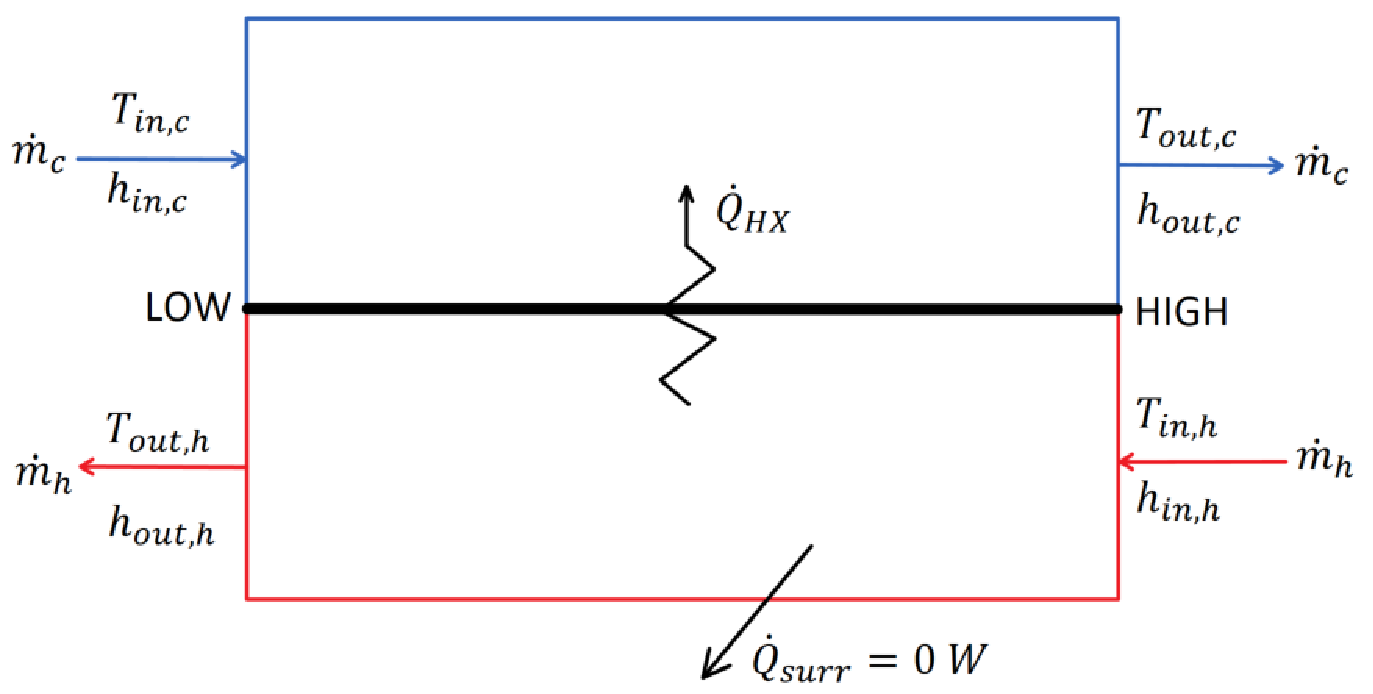
\includegraphics[width=10 cm]{Definitions/counter-flow-hx.pdf}
    \caption{Simplified counter-flow heat exchanger~diagram. \label{counter-flow-hx}}
\end{figure}
% \begin{paracol}{2}
% %\linenumbers
% \switchcolumn

Additional assumptions of the counter-flow heat exchanger model are: no heat loss to the surroundings, no pressure drops across the heat exchangers, and~no fouling resistances. In~Figure~\ref{counter-flow-hx}, the subscript 'out' denotes where the streams are leaving, 'in' denotes the entering streams, 'c' and 'h' signify cold and hot streams respectively, $\dot{Q}_{HX}$ is the total heat transfer from the hot to cold stream, and~$\dot{Q}_{surr}$ is the heat transfer to the~surroundings.

Counter-flow heat exchanger calculations require two known state points, fluid properties, mass flow rate of hot and cold side, and~a specified approach temperature. In~the modeled cases, the~approach temperature is set to value of $10~^{\circ}$C, based off prior model development of sCO$_{2}$ Brayton cycle heat exchangers~\cite{seidel_2010_model_development}. The~fluid libraries referenced are built into %\replaced[comment={Abbreviation defined [4,1]}]
{Engineering Equation Solver (EES)}
%{EES} 
for Carbon Dioxide and Salt (60\% NaNO$_3$ 40\% KNO$_3$) \cite{pacheco_1995_salt_properties,roland_1996_CO$_2$_properties}. 

To analyze the counter-flow heat exchanger, a side is chosen, usually the high side, to~start the calculations. The~approach temperature is initially subtracted from the hot stream on the high-temperature side to find the missing cold temperature according to \mbox{Equation (\ref{temp_h}).}
\begin{equation}
   \label{temp_h}
    T_{out,c} = T_{in,h}-\Delta_{T},
\end{equation}
where T$_{out,c}$ is the cold stream outlet temperature and T$_{in,h}$ is the hot stream inlet temperature. Knowing the two state points allows for the enthalpy out to be found using correlations from the fluid property libraries. This enthalpy then allows for the heat transfer of the heat exchanger to be found with Equation~(\ref{heattrans_h}).
\begin{equation}
    \label{heattrans_h}
     \dot{Q}_{HX} = \dot{m}_{c}(h_{out,c}-h_{in,c}),
 \end{equation}
where $\dot{Q}_{HX}$ is the total heat transfer rate from the hot stream to the cold stream, $\dot{m}_{c}$ is the mass flow rate of the cold stream, $h_{out,c}$ is the enthalpy at the outlet of the cold side, and~$h_{in,c}$ is the inlet of the cold side.
 The known heat transfer of the counter-flow heat exchanger can then solve for the enthalpy out of the hot stream, h$_{out,h}$. This is accomplished with Equation~(\ref{enthalpy_h}).
\begin{equation}
    \label{enthalpy_h}
     h_{out,h} = h_{in,h} - \frac{\dot{Q}_{HX}}{\dot{m}_{h}},
 \end{equation}

Knowing the hot stream enthalpy out allows for all states to be set on the outlets and inlets of the counter-flow heat exchanger. The~temperature difference of the low side is then checked to ensure that it is larger than the approach temperature, defined at $10~^\circ$C. If~the temperature difference on the low side is smaller than the approach temperature, the~same computations are carried with the low side as the starting~point.

Knowing the state points on all inlets and outlets of the counter-flow heat exchanger allows for the heat exchanger performance metrics to be calculated. Performance metrics include %\replaced[comment={Abbreviations defined [4,1]}]
{effectiveness ($\varepsilon$), capacitance (CR), conductivity (UA), and~number of transfer units (NTU).}
%{effectiveness, capacitance, UA, and NTU} 
for heat exchangers. Effectiveness is the ratio of the actual heat transfer rate to the maximum heat transfer rate, %\replaced[comment={sentence proofread}]
{a perfect heat exchanger has an effectiveness of one}
%{or a perfect heat exchanger} 
with no approach temperature. Assuming the approach temperature is on the high side, the~maximum heat transfer rate, $\dot{Q}_{max}$ is found with the maximum enthalpy. Maximum enthalpy of the cold stream is found with correlations by setting the temperature to T$_{in,h}$ with same pressure on the cold outlet. Using the maximum enthalpy, $h_{max}$, the~maximum heat transfer rate is calculated using Equation~(\ref{heattrans_max}).
\begin{equation}
    \label{heattrans_max}
    \dot{Q}_{max} = \dot{m}_{c}(h_{max}-h_{in,c}),
\end{equation}

Calculating the maximum heat transfer rate allows for effectiveness to be calculated using the ratio in Equation~(\ref{effective}).
\begin{equation}
    \label{effective}
    \varepsilon = \frac{\dot{Q}_{HX}}{\dot{Q}_{max}},
\end{equation}

All of the prior equations are carried out in a built-in function within EES. EES is an iterative solver, and therefore if there is a feasible solution, the~functions can take any of the four state points around the heat exchanger and converge on a~solution.

After the effectiveness is solved for, capacitance ratio is necessary. The~capacitance ratio is defined as the average minimum capacitance rate, $\dot{C}_{min}$, over~the average maximum capacitance rate, $\dot{C}_{max}$. Average capacitance rates for the hot and cold streams are found by multiplying the addition of the specific heat at the inlet and outlet of the stream by the mass flow and dividing by two as shown in Equation~(\ref{avg_cap}).
\begin{equation}
    \label{avg_cap}
    \dot{C}_{avg} = \frac{\dot{m}(c_{in}+c_{out})}{2},
\end{equation}
where $\dot{C}_{avg}$ is the average capacitance rate across the hot or cold stream and $c_{in}$ and $c_{out}$ is the specific heat at the inlet and outlet respectively. %\replaced[comment={Improving counter-flow hx explanation [1,1]}]
{Specific heat is found using library correlations, with~the average capacitance rate assumed to be constant during the analysis.}
%{Specific heat is found using library correlations.} 
Once both average capacitances are calculated for the hot and cold streams, one has a larger value, $\dot{C}_{max}$, and~one has a smaller value,  $\dot{C}_{min}$. These maximum and minimum values are used to find the capacitance ratio, $CR$, in~Equation~(\ref{cap_ratio}).
\begin{equation}
    \label{cap_ratio}
    CR = \frac{\dot{C}_{min}}{\dot{C}_{max}},
\end{equation}

%\replaced[comment={Improving counter-flow hx explanation [1,1]}]
{Assuming constant average capacitance rate is suitable for most engineering purposes, especially when there is uncertainty associated with other design parameters~\cite{nellis_klein_2008}. To~justify the assumption of constant average capacitance rate, two graphs for the LTR and HTR are plotted. To~ensure that there is no internal pinch point, the~temperatures of the hot and cold streams as a function of dimensionless length in the LTR and HTR are shown in Figure~\ref{graphs-t-c-vs-p}b,d respectively. Additionally, to~confirm approximate linearity of specific heats at differential steps throughout the counter-flow heat exchanger, the~specific heat as a function of dimensionless length of the hot and cold streams in the LTR and HTR are plotted in Figure~\ref{graphs-t-c-vs-p}a,c respectively.}%{} 

%\replaced[comment={Improving counter-flow hx explanation [1,1]}]
{The calculations used to discretize the counter-flow heat exchangers into a sub-heat exchanger model, shown in Figure~\ref{graphs-t-c-vs-p}, is from Dyreby~\cite{dyreby_2014}. Figure~\ref{graphs-t-c-vs-p} is constructed using the most extreme temperature values experienced by the recuperators---the cold inlet and hot outlet are the lowest and highest modeled temperature values, respectively. As~demonstrated, the~capacitance ratio determines the approach temperature instead of any possible internal pinch point within the recuperator. All pinch points recorded are on the high-temperature end.}{}
\end{paracol}

\clearpage
\begin{figure}[H]
    \begin{subfigure}[b]{0.48\textwidth}
        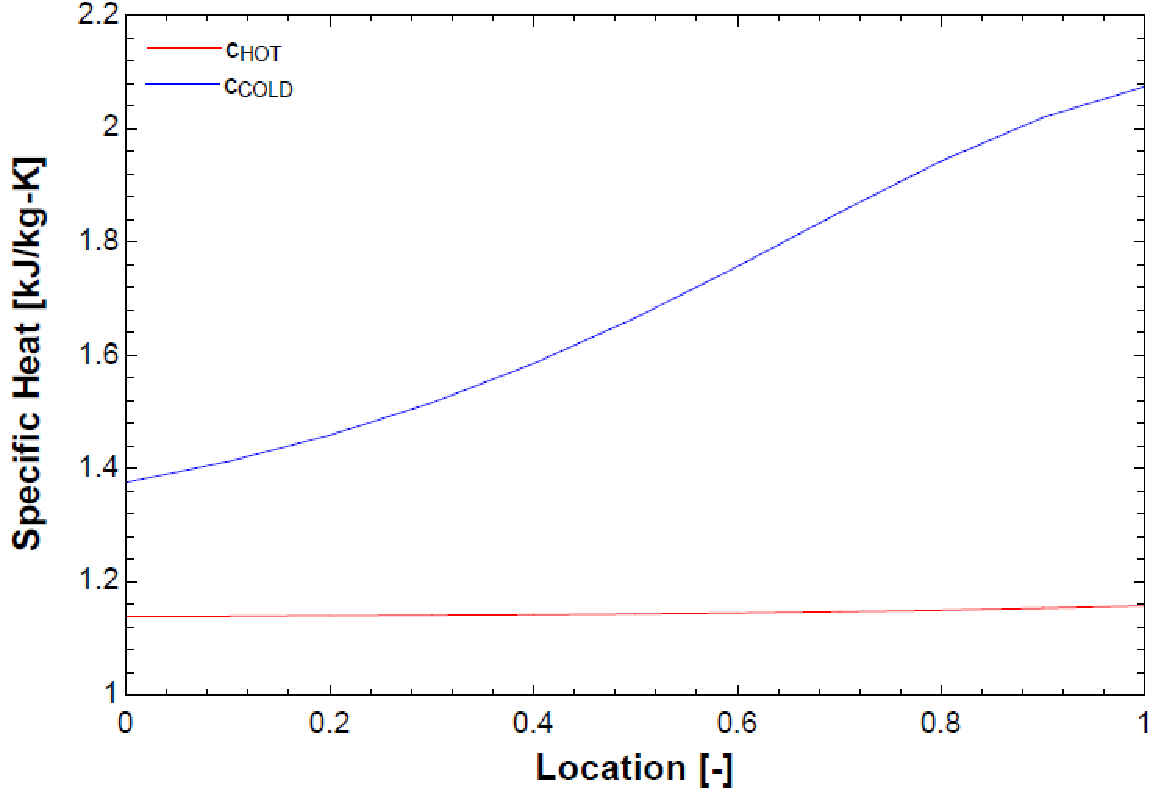
\includegraphics[width=\textwidth]{Definitions/c-vs-p-ltr.pdf}
        \caption[]%
        {{\small }}
        \label{graph-c-vs-p-ltr}
    \end{subfigure}
    \hfill
    \begin{subfigure}[b]{0.48\textwidth}
        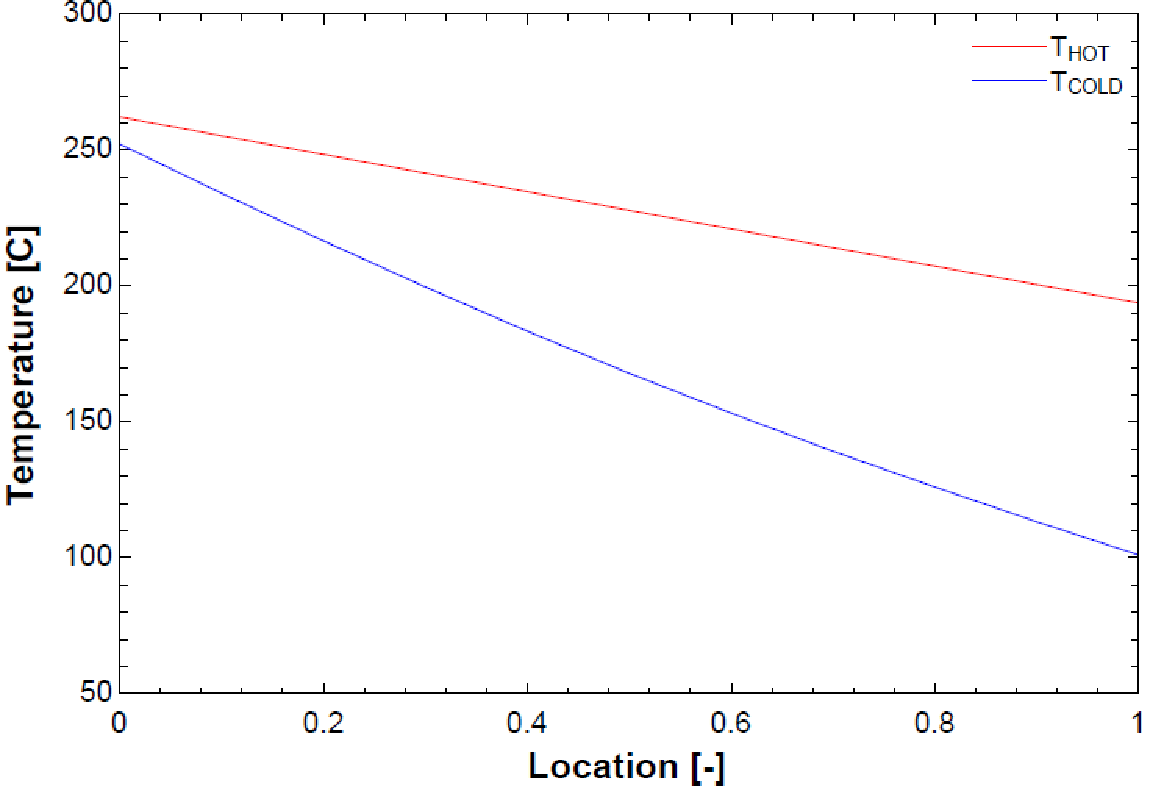
\includegraphics[width=\textwidth]{Definitions/t-vs-p-ltr.pdf}
        \caption[]%
        {{\small }}
        \label{graph-t-vs-p-ltr}
    \end{subfigure}
    \vskip\baselineskip
    \begin{subfigure}[b]{0.48\textwidth}
        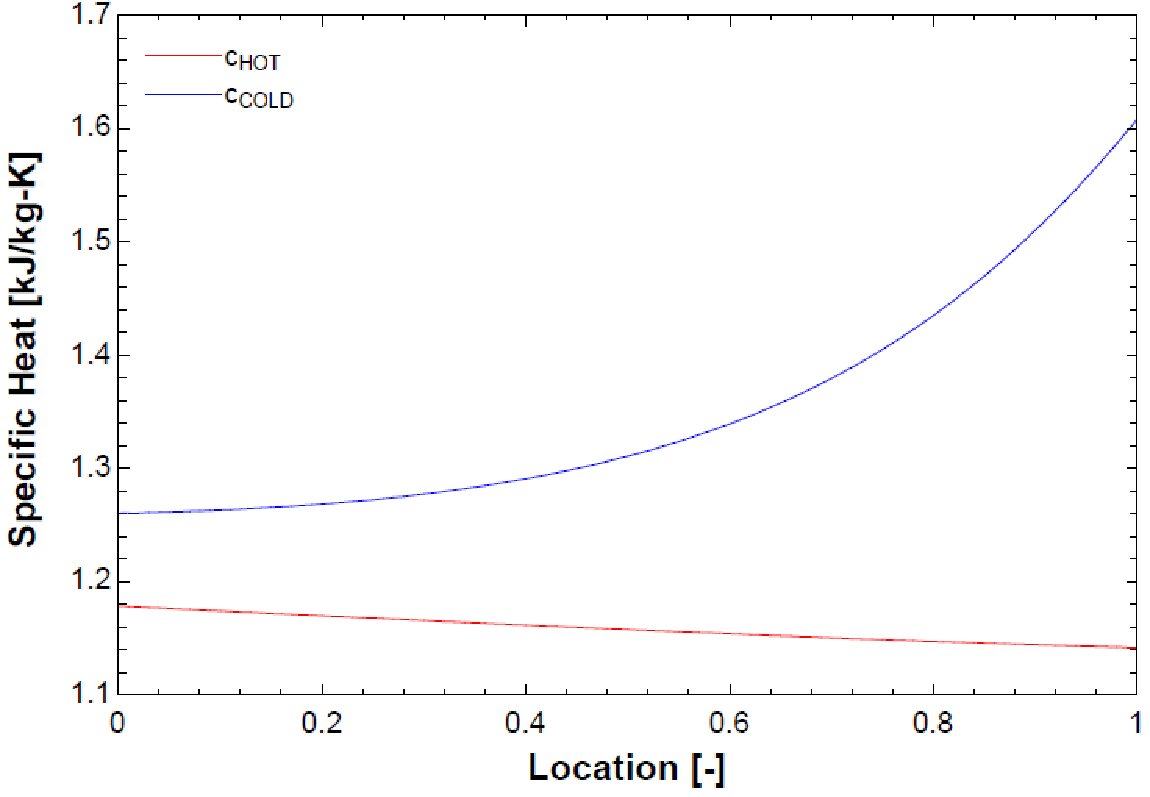
\includegraphics[width=\textwidth]{Definitions/c-vs-p-htr.pdf}
        \caption[]%
        {{\small }}
        \label{graph-c-vs-p-htr}
    \end{subfigure}
    \hfill
    \begin{subfigure}[b]{0.48\textwidth}
        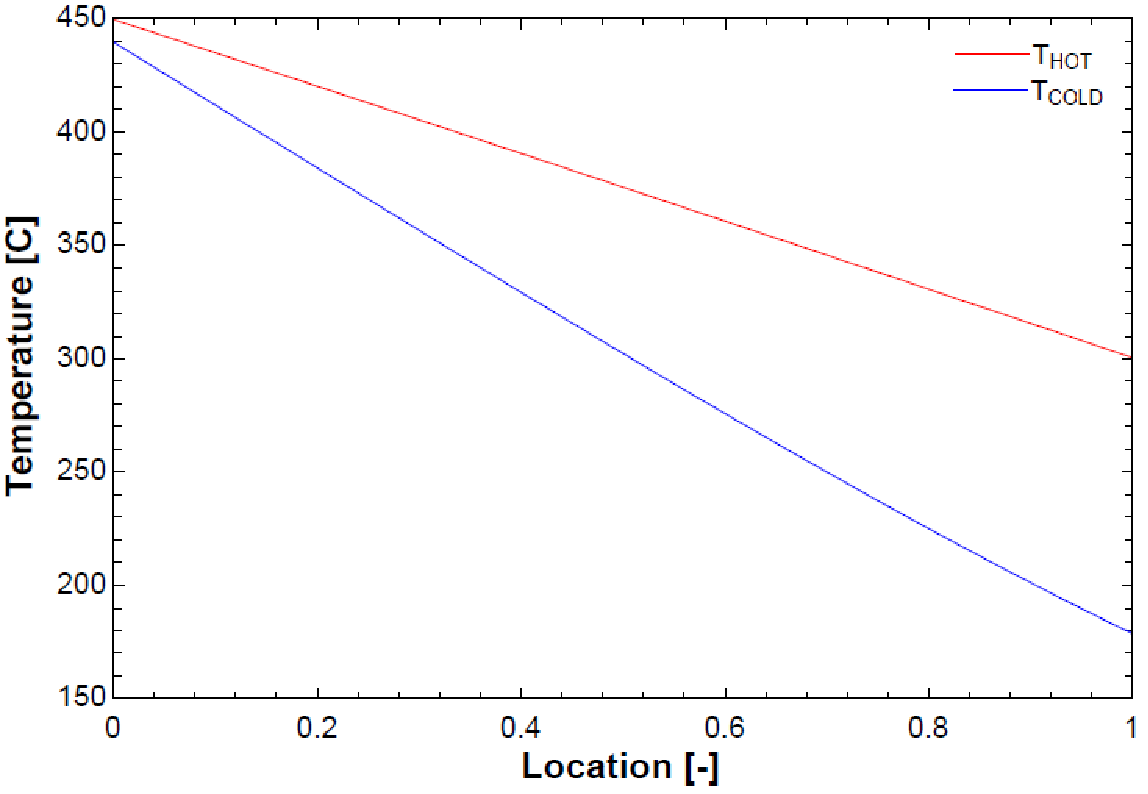
\includegraphics[width=\textwidth]{Definitions/t-vs-p-htr.pdf}
        \caption[]%
        {{\small }}
        \label{graph-t-vs-p-htr}
    \end{subfigure}
    \caption{Specific heats and temperatures of hot and cold streams as a function of dimensionless location for the low-temperature recuperator and high-temperature recuperator. (\textbf{a}) Specific heat as a function of location for LTR; (\textbf{b}) temperature as a function of location for LTR; (\textbf{c}) specific heat as a function of location for HTR; (\textbf{d}) temperature as a function of location for~HTR.}
    \label{graphs-t-c-vs-p} 
\end{figure}

\begin{paracol}{2}
  %%\linenumbers
    \switchcolumn


\vspace{-6pt}
\subsubsection{Lead-Cooled Fast~Reactor}
%--------------------------------------------------------------------------------------
Lead-cooled fast reactors use energy from a controlled nuclear reaction to heat molten lead. This lead is used to cool the core and transfer heat into the sCO$_2$ Brayton power cycle~\cite{smith_2016_lfr_background,alemberti_2013_lfr_overview}. The~lead-cooled fast reactor is assumed to be a black box heat transfer and is labeled in the cycle models LFR HX. The~inlet, outlet and heat transfer rates are provided by our industry partner, Westinghouse, making the black box simplification viable. The~energy balance for the black box assumption can be seen in Equation~(\ref{eq-lfr-black-box}).
\begin{equation}
    \label{eq-lfr-black-box}
    \dot{m} \cdot h_{inlet} + \dot{Q}_{LFRHX} = \dot{m} \cdot h_{outlet},
\end{equation}
where the left hand side, $\dot{m}$, $h_{inlet}$, and~$\dot{Q}_{LFRHX}$, is the energy into the flow and the right hand side, $\dot{m}$ and $h_{outlet}$, is the energy brought out from the flow of sCO$_2$. The~amount of energy transferred into the cycle, $\dot{Q}_{LFRHX}$, is set at $950$ MW, and~outlet temperature of the sCO$_2$ from the LFR HX is set at a value of $595~^{\circ}$C. The~outlet temperature of the LFR is specified because of high-temperature material limits on the LFR lead side. The~low-temperature side is allowed to vary over a range of values with some considerations. The~lead flow velocity is limited by the erosion of the fuel, the~slower the lead flow velocity reduces fuel erosion and therefore leads to a more desirable compact design. %\replaced[comment={Edited sentence for clarity [2,3]}]
{At constant lead velocity (and hence mass flow rate), reducing sCO$_2$ inlet temperature allows for a higher coolant temperature increase in the LFR core and hence a higher thermal power output}
%{Restricting the lead flow velocity, and therefore lead mass flow rate, leads to a higher LFR power output when the inlet sCO$_2$ temperature is reduced.} 
LFR sCO$_2$ inlet temperature has a lower bound of 340~$~^{\circ}$C before the lead begins to freeze, which is operationally unacceptable. When the inlet temperature of sCO$_2$ is increased the temperature difference across the LFR is decreased leading to an increase in power conversion cycle thermodynamic efficiency but a reduction in LFR power below $950$ MW. There is a compromise between high LFR efficiency and LFR power, and therefore a temperature of 400~$~^{\circ}$C for the sCO$_2$ inlet temperature is the optimal value provided by~Westinghouse.


\subsubsection{Concentrating Solar Power~Cycle}
%--------------------------------------------------------------------------------------

The CSP salt cycle modeled in this paper is composed of hot and cold thermal energy storage, %\replaced[comment={Removed Abbreviation [4,1]}]
{}
%{(TES)}
pumps, receiver, sCO$_2$-to-salt counter-flow heat exchanger (C2S), and~CSP counter-flow heat exchanger (CSP HX). The~diagram for this CSP salt loop is shown in Figure~\ref{csp}. 

% \end{paracol}


\begin{figure}[H] 
    %[htb]
    %\widefigure
    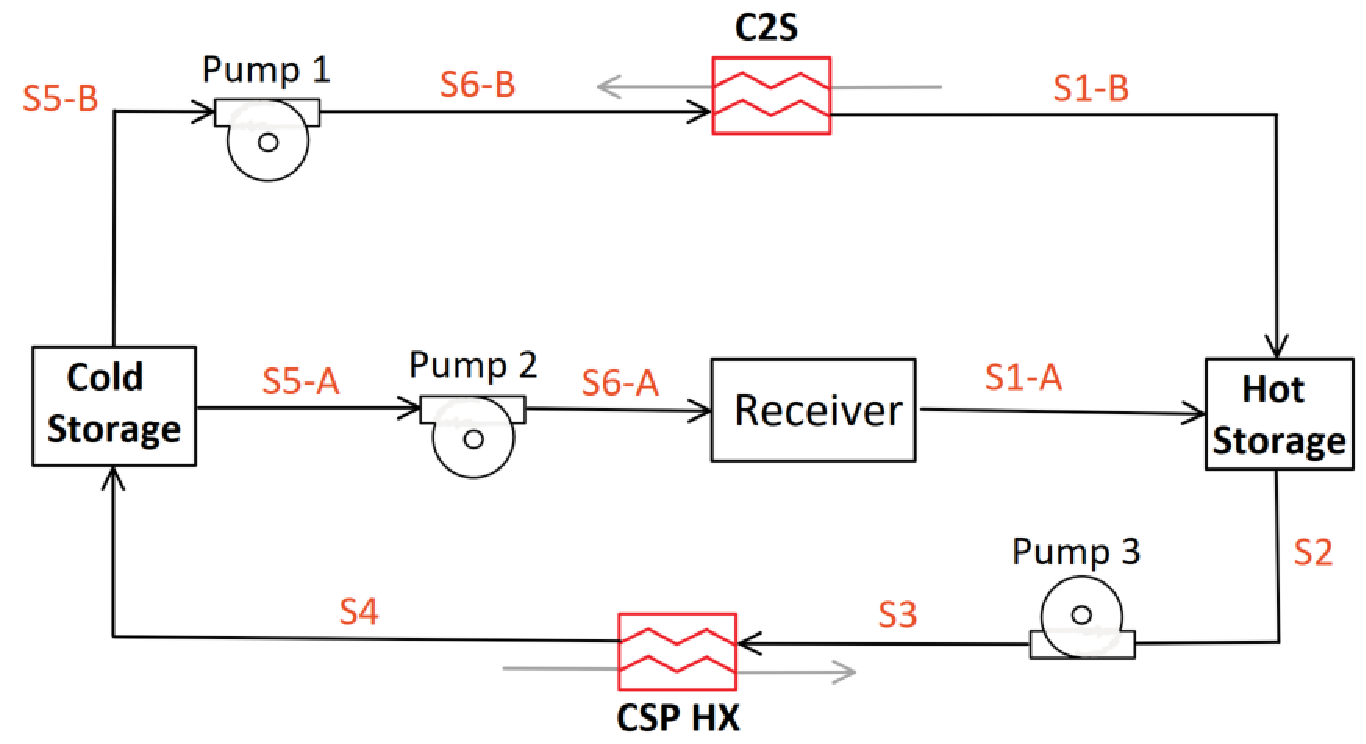
\includegraphics[width=10 cm]{Definitions/csp.pdf}
    \caption{Diagram for CSP cycle with cold and hot thermal energy storage, pumps, and~csp black box heat~input\label{csp}}
\end{figure}
% \begin{paracol}{2}
% %\linenumbers
% \switchcolumn

The CSP salt cycle uses 60\% sodium nitrate, NaNO$_3$, and~40\% potassium nitrate, KNO$_3$, 'solar salt' as the heat transfer fluid. Solar salt stored in the hot TES can be dispatched on demand through the CSP HX when grid demand increases and held when grid demand is low. Current CSP salt cycles heat solar salt with receivers and store it in hot TES tanks at temperatures around 565$~^{\circ}$C. Future CSP salt cycles are hypothesized to have bulk hot TES temperatures of up to $720~^{\circ}$C, but~here the hot TES temperature is set at $560~^{\circ}$C for all modeled cycles~\cite{mehos2017concentrating} as this has been commercially proven. The~cold TES temperature takes on three different values according to cycle configuration capabilities: $390~^{\circ}$C, $410~^{\circ}$C, and~$440~^{\circ}$C. In~addition to the lower hot TES temperature, current CSP salt cycles lack a secondary option for charging the hot TES~\cite{hamilton2020dispatch}. The~studied CSP salt cycle has two TES charging options: a receiver, which generates heat from a heliostat field, and~C2S heat exchanger, which draws excess heat from the sCO$_2$ Brayton cycle. While the hot TES is charging, the~receiver and LFR are storing heat for later use when grid demand increases. The~hot TES storage is not dispensing salt for use in the CSP cycle while~charging.

The C2S heat exchanger is active in the 'charging' cycle operating modes, when the focus is on heat storage for later use. Pump 1 is actively moving solar salt from cold TES to hot TES through the C2S heat exchanger extracting heat from the sCO$_2$ Brayton cycle. Additionally, while the focus is on heat storage, and~the heliostat field is inputting heat, pump 2 is actively transporting solar salt through the receiver to be stored in the hot~TES.

'Non-charging' cycle operating modes are characterized by operations wherein the CSP salt cycle is discharging the hot TES, the~C2S heat exchanger is not transferring heat, and~the LFR is dispatching heat directly to generate electricity. When electrical generation is occurring and solar resource is available, the~heat input in the CSP salt cycle is modelled through a black box energy balance across states S6-A and S1-A with a heat addition of 750 MW from the heliostat field. The~hot TES solar salt is moved through Pump 3 and transfers heat into the sCO$_{2}$ Brayton cycle through CSP HX to be converted into electricity. The~cooled salt is stored in cold storage and moved through Pump 2, where the heat from the receiver is again transferred into the CSP~cycle. 

When grid demand for electrical power increases, a~series of operating modes are activated. During~the highest demand times, cycle operation focuses on maximum electrical generation. This is achieved through the C2S being turned off for direct electrical production from the LFR and the hot TES is discharging heat through the CSP HX for electrical production in the sCO$_2$ Brayton cycle. %\replaced[comment={Edited sentence to clarify that the CSP charges the hot TES during low grid demand periods [2,4]}]
{As grid demand diminishes, CSP HX ramps down heat extraction until no power is being dispatched through the salt and the hot TES begins charging. During~this process, the~LFR gradually adds a larger fraction of heat input to the TES through C2S, supplementing the heat produced by the CSP which is also used to charge the TES. This process continues until no electrical production is occurring in the cycle and all heat is stored in TES for later use.}
%{As grid demand diminishes, CSP HX ramps down heat extraction until no power is being dispatched through the salt and the hot TES begins charging. During this process, the LFR gradually adds a larger fraction of heat input to the TES through C2S. This process continues until no electrical production is occurring in the cycle and all heat is stored in TES for later use.} 



\subsection{Standardization of Cycle~Modeling}
%======================================================================================


In order to draw a more direct comparison, the~cycles are standardized in terms of isentropic efficiencies, heat exchanger approach temperatures, pressures, heat input, and~pump constants. These values are summarized in Table~\ref{tab-cycle-constants}.

\begin{specialtable}[H] 
    %[htbp]
    \caption{Standardized constant cycle parameters with definition, variable and set~value. \label{tab-cycle-constants}}
    \begin{tabular}{L{0.52\linewidth}cc}
    \toprule
    \textbf{Parameter} & \textbf{Variable}	& \textbf{Design Point Value}\\
    \midrule
    \textit{\hl{Efficiencies} %Is the italics necessary?
}\\
    Main Compressor & $\eta_{MC}$		& 0.91 (-)\\
    Re-Compressor & $\eta_{RC}$		& 0.89 (-)\\
    Turbine & $\eta_{T}$		& 0.90 (-)\\
    Pumps 1--3 & $\eta_{P}$      & 0.90 (-)\\
    \midrule
    \textit{Approach Temperatures}\\
    Low-Temperature Recuperator & $\delta_{LTR}$		& 10 ($~^{\circ}$C)\\
    High-Temperature Recuperator & $\delta_{HTR}$		& 10 ($~^{\circ}$C)\\
    Concentrating Solar Power Heat Exchanger & $\delta_{CSPHX}$	& 10 ($~^{\circ}$C)\\
    \midrule
    \textit{Pressures}\\
    Pressure Ratio & $PR$ & 3.27 (-)\\
    High Side Pressure & $P_{2A}$ & 28.8 (MPa)\\
    \midrule
    \textit{Heat into System}\\
    Lead-Cooled Fast Reactor Heat Transfer & $\dot{Q}_{LFRHX}$ & 950 (MW)\\
    Concentrating Solar Power Heat Transfer & $\dot{Q}_{CSP}$ & 750 (MW)\\
    \midrule
    \textit{Temperature}\\
    Main Compressor Inlet & $T_{1A}$ & 40 ($~^{\circ}$C)\\
    Lead-Cooled Fast Reactor sCO$_{2}$ High Temperature & $T_{5}$,$T_{2C}$,$T_{6A}$,$T_{5C}$ & 595 ($~^{\circ}$C)\\
    \midrule
    \textit{Pumps}\\
    Pressure Rise across Pump & $\Delta_{P}$ & 3.726 (MPa)\\
    Pump Low Side Pressure & $P_{S5-B}$ & 3 (MPa)\\ 
    \bottomrule
    \end{tabular}
\end{specialtable}

The values displayed in Table~\ref{tab-cycle-constants} are representative of CSP and the Westinghouse LFR. 
%\replaced[comment={Elaborated on table variable names [2,5]}]
{In Table~\ref{tab-cycle-constants}, variable names require further explanation. The~high side pressure with the variable label $P_{2A}$, is the constant pressure outlet on the compressors and inlet to the turbines. In~all models, the value is set by the outlet of the main compressor and held constant with the assumption that there is no pressure drop across heat exchangers. In~addition to this pressure, temperatures are also set. The~inlet temperature of the main compressor, $T_{1A}$, is set to a value of $40~^{\circ}$C in all models. The~temperature of the sCO$_2$ on the outlet of the LFR HX has different variable names, T$_5$, T$_{2C}$, T$_{6A}$, and~T$_{5C}$, according to the associated cycle configuration diagram.}{}


In addition to standardized parameters, all cycles have identical recompression sides. The~recompression side contains a  %\replaced[comment={Abbreviations defined [4,1]}]
{precooler (PC), low-temperature recuperator (LTR), and~two compressors; main compressor (MC) and recompressor (RC)}
%{precooler, low-temperature recuperator, and two compressors; main compressor and recompressor}. 
The modeled cycles are summarized in Table~\ref{tab-cycle_sum}.

\begin{specialtable}[H] 
    \caption{Summary of all modeled non-charging and charging cycles with~descriptions. \label{tab-cycle_sum}}
    \begin{tabular}{lL{0.75\linewidth}}
    \toprule
    \textbf{Cycle Label} & \textbf{Description}\\
    \midrule
    \textit{Non-Charging}\\
    C-LFR-ON & Two-cycle configuration with LFR as heat source.\\
    C-CSP-ON & Two-cycle configuration with CSP as heat source.\\
    C-1HTR1T-ON & CSP and LFR heat sources in parallel with one turbine.\\
    C-2HTR3T-ON & CSP and LFR loops each with dedicated HTR and turbine.\\
    \midrule
    \textit{Charging}\\
    C-LFR-PRE & Turbine is prior to the C2S.\\
    C-LFR-POST & Turbine is after the C2S.\\
    C-LFR-PAR & Turbine is parallel to the C2S.\\
    C-LFR-CIRC & Circulator bridges the LFR and C2S.\\
    \bottomrule
    \end{tabular}
\end{specialtable}

\subsection{Non-Charging Cycle~Configurations} 
%======================================================================================

Various cycles are modeled to test their advantages and disadvantages. These cycle models fall into two categories: non-charging and charging. The~non-charging category is used to determine the configuration of the cycle with a focus on electricity generation. This includes the number and location of turbines, recuperators, and~heat input to the system by the CSP and LFR. To~quantify the effectiveness of the non-charging configurations, a~cycle efficiency, $\eta_{cycle}$, is defined in Equation~(\ref{eq-eta-cycle}).
\begin{equation}
    \label{eq-eta-cycle}
    \eta_{cycle} = \frac{\dot{W}_{T}-\dot{W}_{MC}-\dot{W}_{RC}}{\dot{Q}_{LFRHX}+\dot{Q}_{CSPHX}},
\end{equation}

The numerator in Equation~(\ref{eq-eta-cycle}) is the alternator power, or~the power produced from the turbines, $\dot{W}_{T}$, minus the required power of the compressors, $\dot{W}_{MC}$ and $\dot{W}_{RC}$. The~denominator is the total power input into the system from the LFR HX, $\dot{Q}_{LFRHX}$, and~CSP HX, $\dot{Q}_{CSPHX}$.


\subsubsection{Two-Cycle Configuration: C-LFR-ON and~C-CSP-ON} %--------------------------------------------------------------------------------------

The two-cycle configuration that is tested has independent sCO$_{2}$ loops that share a common CSP salt cycle. This cycle has two sCO$_{2}$ Brayton Cycles: C-LFR-ON and C-CSP-ON. Configuration of components for these two cycles is identical with the exception of heat inputs. C-LFR-ON has heat provided from a LFR while C-CSP-ON has heat provided from the CSP. These two cycles individually operate when the focus of plant operation is primarily electricity~generation. 
    
The cycle that is using the LFR heat input in the two-cycle configuration is labeled as C-LFR-ON and the cycle diagram is illustrated in Figure~\ref{c-lfr-on}. 

Two separate sensitivity studies on the LFR inlet temperature are completed for C-LFR-ON. The~constrained study is calculated by setting the LFR inlet temperature to the design value of $400~^{\circ}$C, which is a requirement of the LFR primary circuit to maximize power output within material limits. In~addition to the constrained studies, unconstrained studies are required to test the penalties that LFR inlet temperature has on efficiency. The~unconstrained study is performed by gradually increasing the mass flow to the main compressor through a parametric study while maximizing cycle efficiency. In~Figure~\ref{c-lfr-on}, the~location of the C2S heat exchanger while charging falls between state point 5 and 6 in any of the studied charging configurations: parallel, pre, circulator or~post. 

 \end{paracol}
\begin{figure}[H] 
    %[!h] 
  % \widefigure
    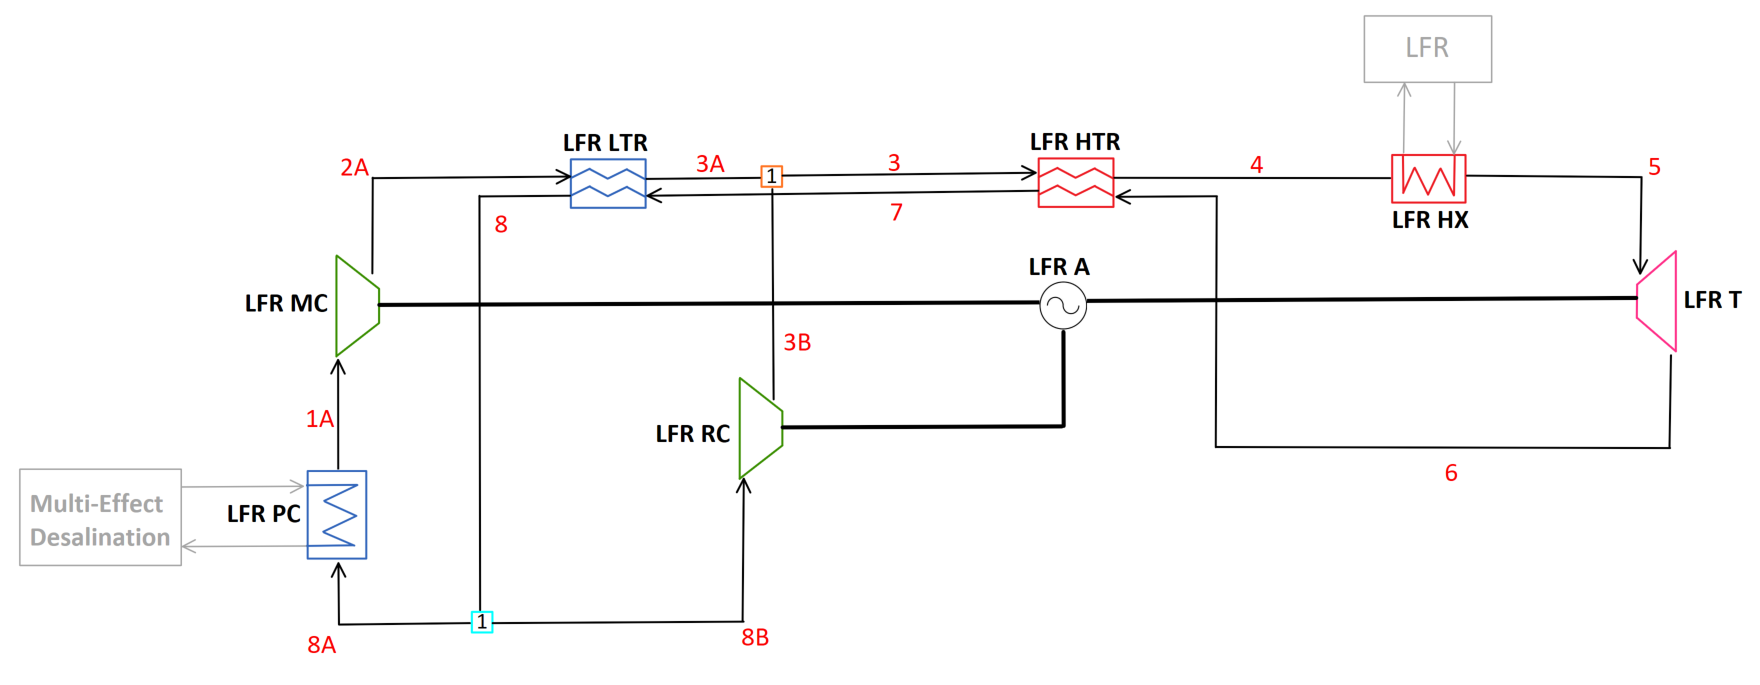
\includegraphics[width=\linewidth]{Definitions/c-lfr-on.pdf}
    \caption{Diagram for C-LFR-ON with focus on electricity~generation\label{c-lfr-on}}
\end{figure}
 \begin{paracol}{2}
% %\linenumbers
 \switchcolumn

The cycle that is using the CSP heat input in the two-cycle configuration is labeled C-CSP-ON and the cycle diagram is shown in Figure~\ref{c-csp-on}. 

%\clearpage
\end{paracol}
\begin{figure}[H] 
    %[!h]
    \widefigure
    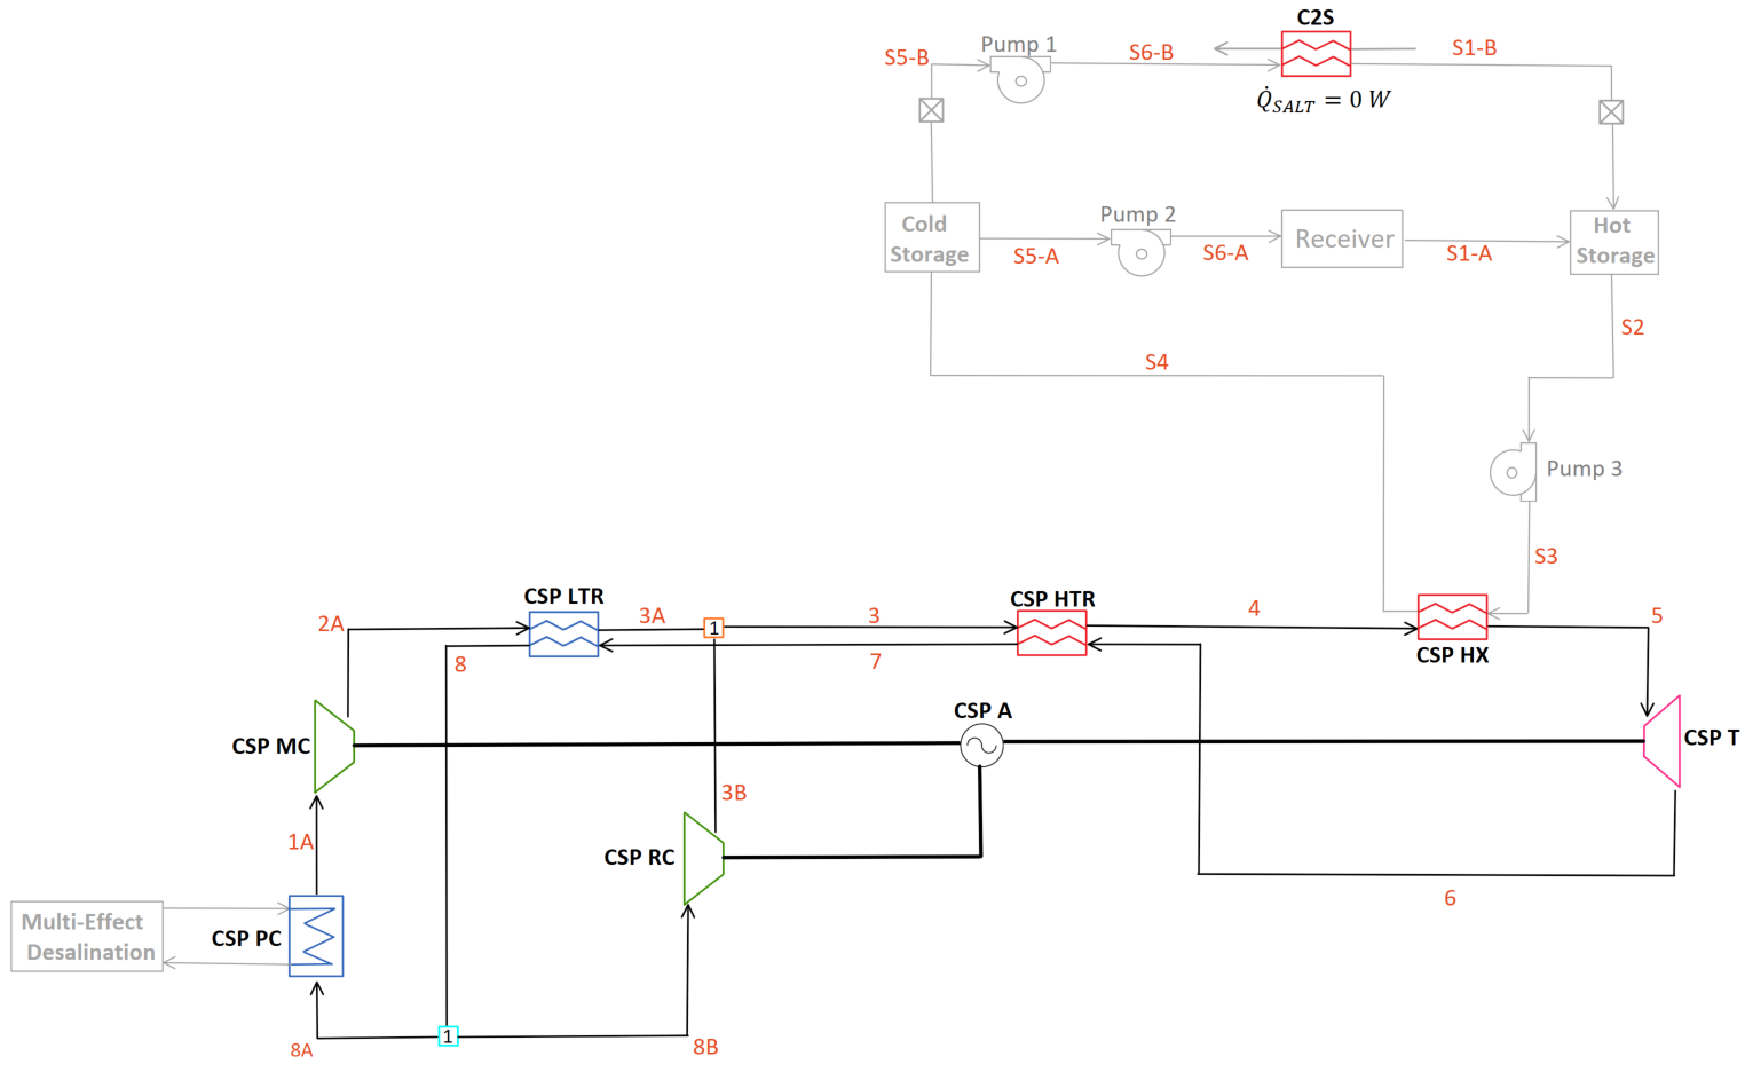
\includegraphics[width=\linewidth]{Definitions/c-csp-on.pdf}
    \caption{Diagram for C-CSP-ON with focus on electricity~generation\label{c-csp-on}}
\end{figure}
\begin{paracol}{2}
%%\linenumbers
\switchcolumn

 Due to the individual operation while the cycles are generating electricity, C-CSP-ON is not directly impacted by the LFR low-end temperatures. Instead, a~sensitivity study is performed on the temperature of the cold TES. Two temperatures are tested, $390~^{\circ}$C and $440~^{\circ}$C, to~observe the impact of cold TES temperature on cycle efficiency. Efficiencies need to be combined to draw a comparison of the two-cycle configurations to the single-cycle configurations; C-1HTR1T-ON and C-2HTR3T-ON. Equation~(\ref{eq-eta-2cycle}) is used to calculate this combined two-cycle efficiency.
\begin{equation}
    \label{eq-eta-2cycle}
    \eta_{combined} = \frac{\dot{W}_{A,C\text{-}LFR\text{-}ON}+\dot{W}_{A,C\text{-}CSP\text{-}ON}}{\dot{Q}_{LFRHX}+\dot{Q}_{CSPHX}},
\end{equation}

Equation~(\ref{eq-eta-2cycle}) is the ratio of total alternator (net) power of C-LFR-ON, $\dot{W}_{A,C\text{-}LFR\text{-}ON}$, and~C-CSP-ON, $\dot{W}_{A,C\text{-}CSP\text{-}ON}$, to~the total heat input into the cycles from the LFR and CSP heat exchangers, $\dot{Q}_{LFRHX}+\dot{Q}_{CSPHX}$.




\subsubsection{C-1HTR1T-ON} 
%--------------------------------------------------------------------------------------

One drawback of having a two-cycle design, as~seen in the C-LFR-ON and C-CSP-ON, is doubling the number of system components. Combining the two cycles into one would reduce redundancy, complexity, and~cost. Heat addition from the CSP HX and LFR HX in parallel orientation is therefore studied in the C-1HTR1T-ON model. This model studies what impact mixing different temperature flows prior to the turbine has on cycle efficiency. The~diagram for this cycle is illustrated in Figure~\ref{c-1htr1t-on}.
%\clearpage
\end{paracol}

\begin{figure}[H] 
    \widefigure
    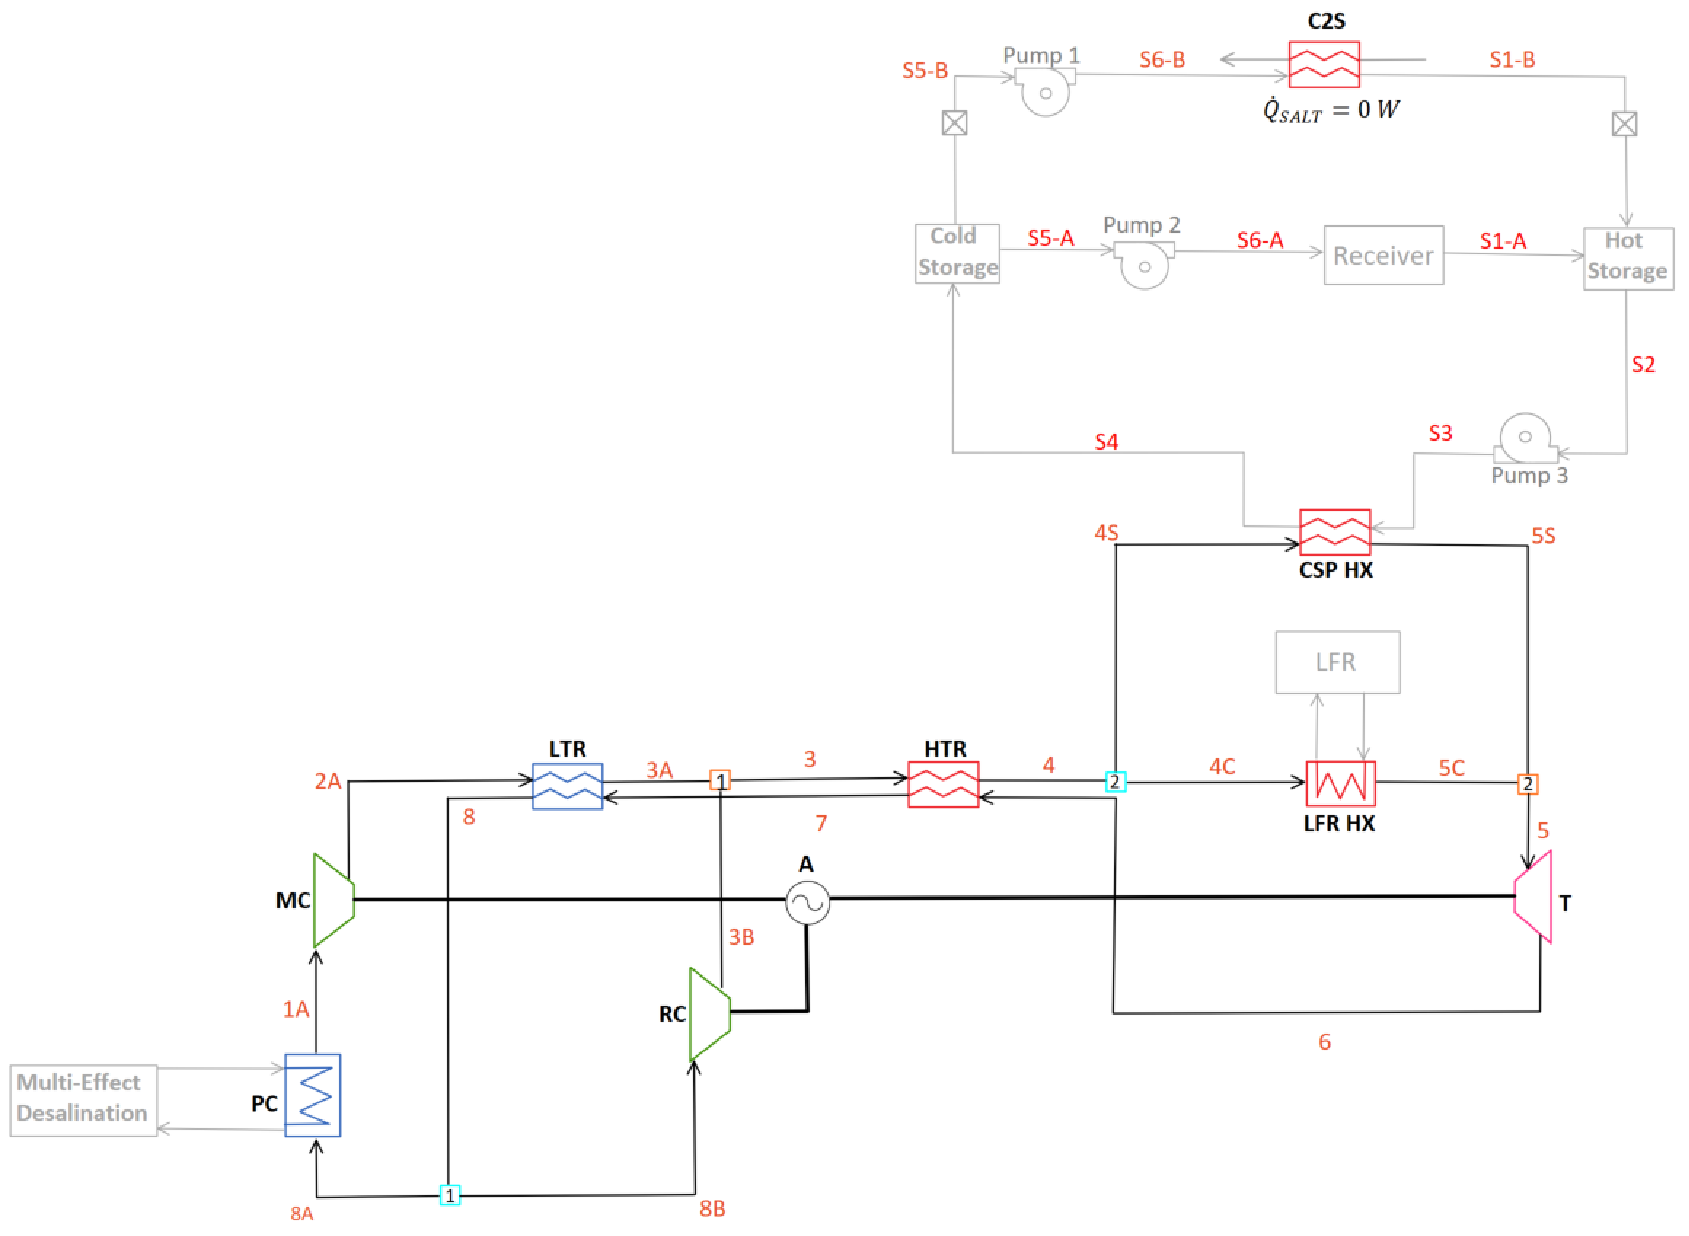
\includegraphics[width=\linewidth]{Definitions/c-1htr1t-on.pdf}
    \caption{Diagram for C-1HTR1T-ON with focus on electricity~generation\label{c-1htr1t-on}}
\end{figure}


\begin{paracol}{2}
%%\linenumbers
\switchcolumn

The C2S is located around the turbine and LFR at state points 5 to 6 depending on the charging cycle configuration: pre, parallel, post or circulator. In~the C-1HTR1T-ON cycle, the~LFR HX and CSP HX have identical inlet temperatures due to splitting the flow prior to their parallel orientation. Therefore, three sensitivity studies are performed on the model. The~initial two studies have the low LFR temperature constrained to the value of $400~^{\circ}$C with varied cold CSP TES temperature and maximized cycle efficiency. To~achieve a maximum cycle efficiency, the~split fraction amount of flow to the main compressor, $y_{1}$, is parametrically studied.
Two cold TES temperatures are tested with constrained LFR low temperature of $400~^{\circ}$C: 
\begin{itemize}
    \item	$410~^{\circ}$C: Lowest cold TES temperature possible due to the sCO$_2$ cold inlet constrained from the LFR to $400~^{\circ}$C and the addition of $10~^{\circ}$C approach temperature;
    \item	$440~^{\circ}$C: Upper bound temperature on cold TES storage;
    \item	$390~^{\circ}$C: Unconstrained LFR cold inlet temperature allows a lower cold TES of $390~^{\circ}$C to be achieved. This allows for a larger temperature drop across the CSP HX, increasing dispatchability.
\end{itemize}


\subsubsection{C-2HTR3T-ON} 
%--------------------------------------------------------------------------------------

The identical inlet temperatures due to the parallel configuration makes the C-1HTR1T-ON cycle configuration restricted. Another single-cycle configuration is desired to allow dissimilar inlet temperatures for the CSP HX and LFR HX while additionally testing the effect that mixing flows downstream from the HTR has on cycle~efficiency. 

In practice, sCO$_2$ cycles typically have 3 turbines, with~2 of these driving the compressor and recompressor. Therefore, this configuration will not in general require additional turbines compared to the C-1HTR1T-ON configuration. Furthermore, it is anticipated that the cost of the high-temperature recuperator (HTR) is likely most related to its volume, and~hence having two smaller high-temperature recuperators is unlikely to cost significantly more than one large~one. 

This cycle, C-2HTR3T-ON, can be seen in Figure~\ref{c-2htr3t-on} and has two high-temperature recuperators and three turbines. The~LFR is powering one turbine, T1, and~transferring unused heat to the flow entering LFR HX through a dedicated high-temperature recuperator, HTR. The~cycle with heat addition from the CSP powers the other two turbines, which for modeling purposes are combined into a single turbine T2, while having a dedicated high-temperature recuperator, HTR2. 

\end{paracol}
\begin{figure}[H]
  \widefigure
  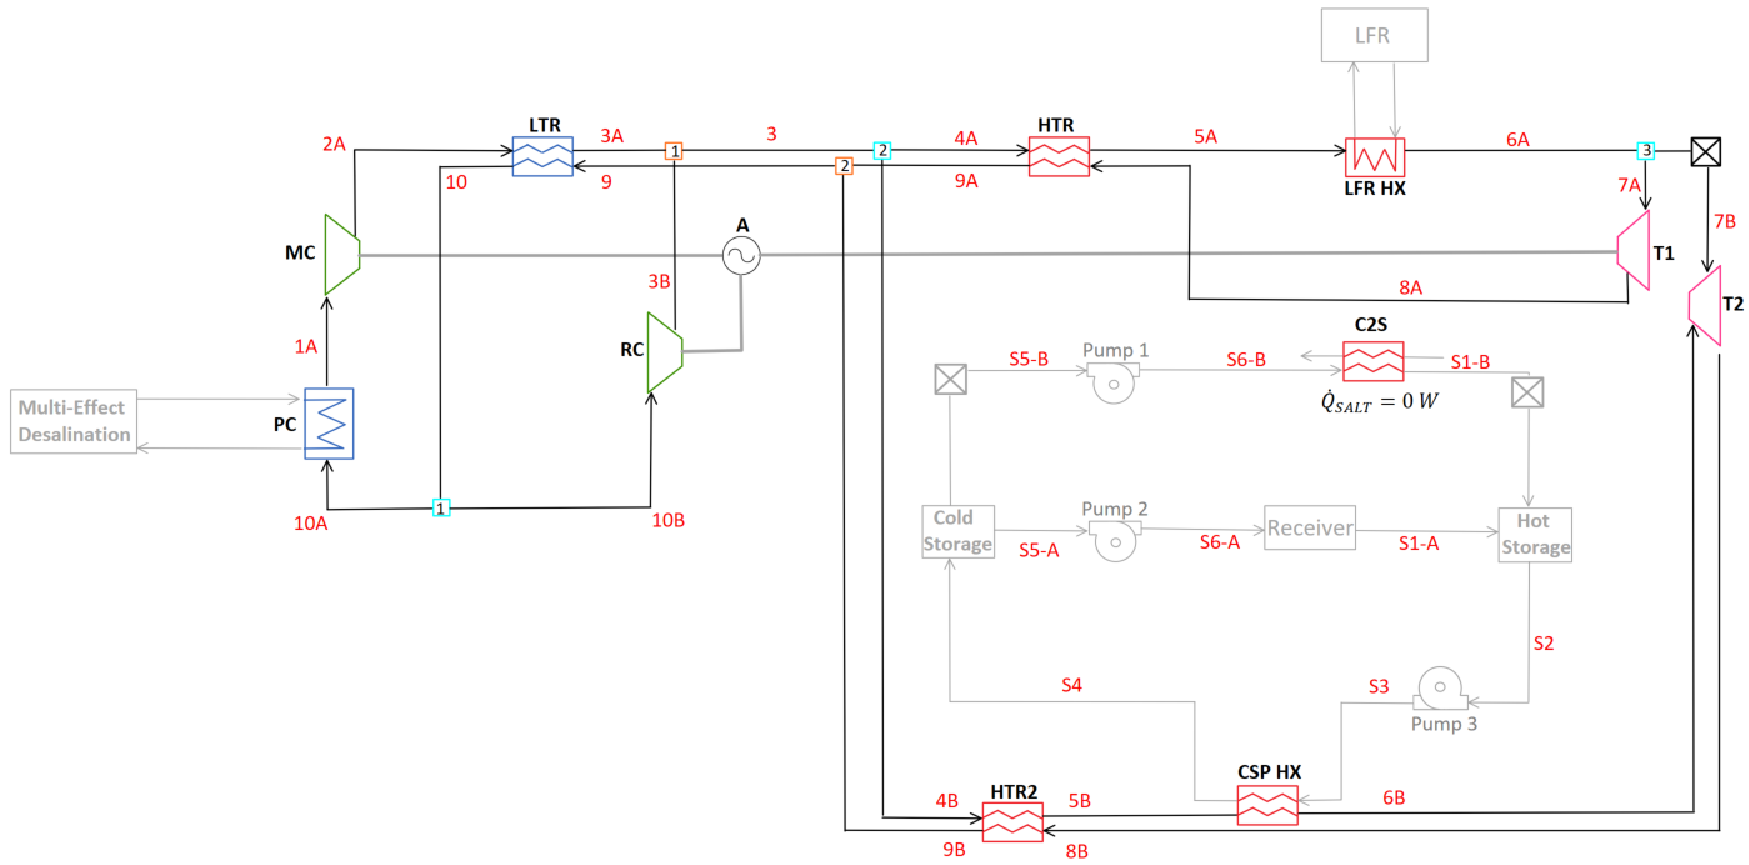
\includegraphics[width=\linewidth]{Definitions/c-2htr3t-on.pdf}
  \caption{Diagram for C-2HTR3T-ON with focus on electricity~generation\label{c-2htr3t-on}}
\end{figure}
\begin{paracol}{2}
  %%\linenumbers
  \switchcolumn
  
  
  The~two turbines displayed as T2 can be modeled as a singular turbine because their isentropic efficiencies are identical causing the inlet and outlet conditions of the turbines to be consistent with a singular turbine. Additionally, the~power produced by the two turbines is proportional to mass flow rate, each receives a fraction of the mass flow rate, therefore producing the same fraction of power. Summing these power fractions together yields the total power of a singular turbine in the same position. After~the high-temperature recuperators, the~two flows are combined and sent to the LTR hot~side. 
  
  The C2S heat exchanger is located around the turbine and LFR at 7A to 8A depending on the charging configuration: pre, post, parallel or circulator. Three sensitivity studies are performed on the C-2HTR3T-ON model---two with the LFR low temperature constrained and one without this constraint. The~two constrained studies, with~an LFR temperature of $400^{\circ}$, have varied cold CSP TES temperature with the lowest temperature of $390~^{\circ}$C and highest temperature of $440~^{\circ}$C. The~unconstrained low LFR inlet study is calculated at a cold CSP TES temperature of $390~^{\circ}$C.



\subsection{Thermal Energy Storage Charging~Techniques} 
%======================================================================================

Charging cycle configurations accommodate energy storage modes of operation. These configurations examine the location of LFR heat extraction via C2S. To~maximize the available heat for extraction, alternator net power is set to zero, therefore requiring the turbine power to balance with the compressors' demand. Despite the components being non-ideal and consuming power, the~recompression cycle continues to operate, ensuring that there is mass flow to transfer heat from the Brayton cycle to C2S. The~excess energy from the LFR is thermally stored in the TES for later use when grid demand increases. Comparison of the heat extraction point in the cycle, C2S, is accomplished by implementing C2S in different locations around the turbine in the C-LFR-ON non-charging cycle configuration; C-LFR-PRE has the turbine prior to C2S, C-LFR-POST has the turbine after C2S, C-LFR-PAR has the turbine in parallel to C2S, and~C-LFR-CIRC uses a circulating loop instead of in-flow implementation. C-LFR-ON is the configuration used for these studies because during charging operation, flow through the CSP HX is deactivated, effectively making all non-charging cycles take the identical form of C-LFR-ON. To~quantify the effectiveness of TES charging techniques, Equation~(\ref{eq-eta-heatstorage}) defines the heat storage efficiency, $\eta_{heatstorage}$.
\begin{equation}
    \label{eq-eta-heatstorage}
    \eta_{heatstorage} = \frac{\dot{Q}_{C2S}}{\dot{Q}_{LFRHX}+\dot{Q}_{CSPHX}},
\end{equation}

In the heat storage efficiency equation, $\dot{Q}_{C2S}$ is the amount of heat transferred through C2S, and~the addition of $\dot{Q}_{LFRHX}$ and $\dot{Q}_{CSPHX}$ is the total amount of heat input into the system from the LFR HX and CSP~HX. 

\subsubsection{C-LFR-PRE} 
%--------------------------------------------------------------------------------------

The high-temperature sCO$_2$ leaving the LFR HX flows through the LFR turbine converting thermal energy to usable work. The~outlet temperature of the LFR turbine is at a temperature suitable to charge the hot TES, and therefore the flow is passed through C2S exchanging heat to the cold solar salt. The~diagram outlining this process is C-LFR-PRE in Figure~\ref{c-lfr-pre}. 

A problem arises with this salt charging configuration. The~temperature out of the turbine is not high enough to charge the hot CSP TES to the required value of $560~^{\circ}$C when the turbine power is balanced with the compressor demand. To~raise the temperature, some of the high-temperature flow before the turbine is redirected through a valve and combined after the turbine. Limiting the flow through the turbine reduces the turbine power and compressor power because of the balancing requirement. Due to the reduction in available compressor power, the~LFR RC is effectively bypassed, and~a large portion of usable heat is expelled in the LFR PC before the LFR MC. The~thermal storage efficiency reduces as a result of the large amount of heat rejected in the LFR~PC.

\end{paracol}
\begin{figure}[H]
    \widefigure
    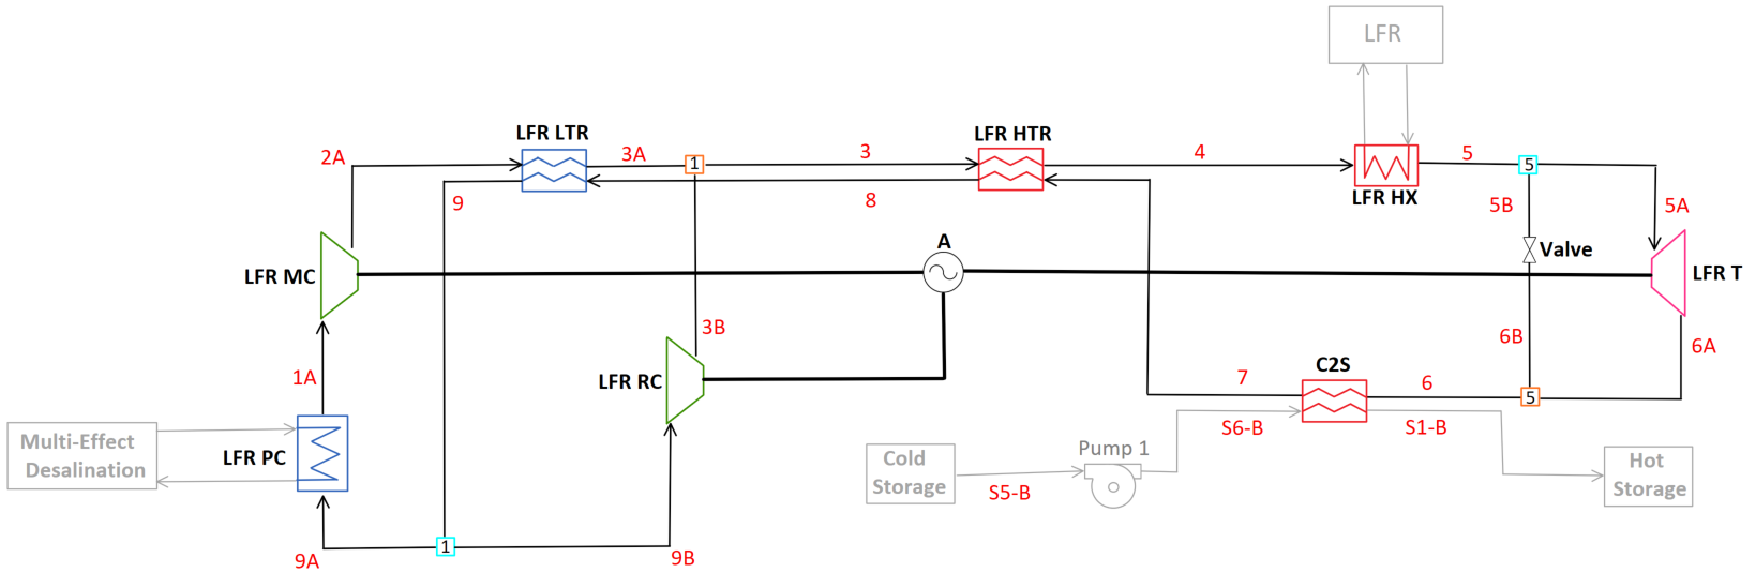
\includegraphics[width=\linewidth]{Definitions/c-lfr-pre.pdf}
    \caption{Diagram for C-LFR-PRE thermal energy storage charging orientation\label{c-lfr-pre}.}
\end{figure}
\begin{paracol}{2}
%%\linenumbers
\switchcolumn




\subsubsection{C-LFR-POST} 
%--------------------------------------------------------------------------------------

Moving the heat extraction prior to the turbine is analyzed in C-LFR-POST. This diagram is shown in Figure~\ref{c-lfr-post}.

\end{paracol}
\begin{figure}[H]
    \widefigure
    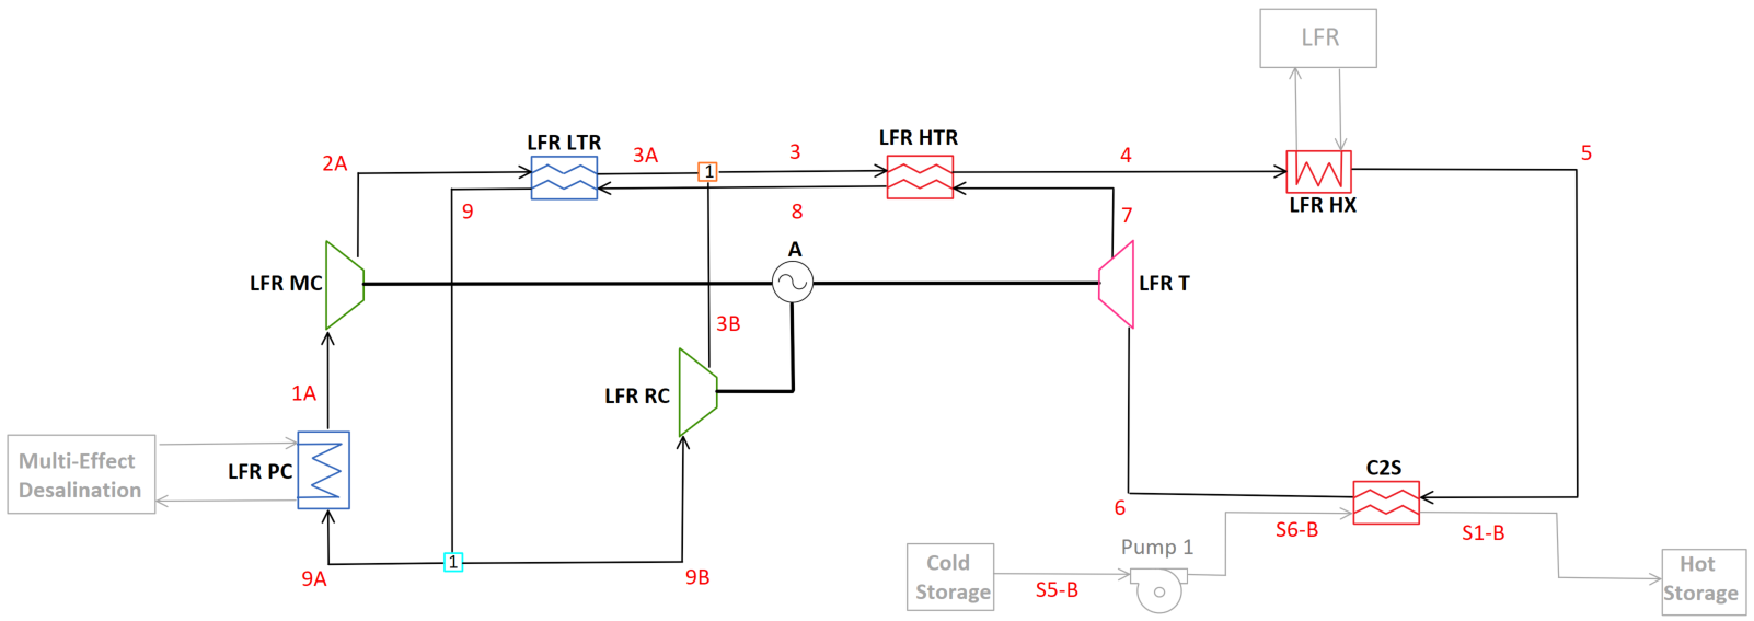
\includegraphics[width=\linewidth]{Definitions/c-lfr-post.pdf}
    \caption{Diagram for C-LFR-POST thermal energy storage charging orientation\label{c-lfr-post}.}
\end{figure}
\begin{paracol}{2}
%%\linenumbers
\switchcolumn

This TES charging cycle extracts heat before the turbine and therefore has a large negative effect on the amount of work that the turbine is producing. The~turbine power offsets the requirements of both compressors, requiring the turbine inlet temperature to be high. The~amount of energy that is extracted before the turbine is small and therefore the heat storage efficiency is fractional compared to other charging techniques. There is no quantitative study performed on this case because, due to the efficiency losses, it is~non-viable. 

\subsubsection{C-LFR-PAR} 
%--------------------------------------------------------------------------------------

The requirements of the turbine and CSP hot TES can be satisfied by splitting the flow before the turbine. The~flow through the salt heat exchanger in this cycle is therefore separate from the turbine. After~the salt heat exchanger, a~valve is needed to reduce the pressure, this TES charging cycle is C-LFR-PAR shown in Figure~\ref{c-lfr-par}.

A sensitivity study with varying cold CSP TES temperature is carried out to determine the impact on heat storage efficiency. The~study considers two temperature values of $390~^{\circ}$C and $440~^{\circ}$C.

\clearpage
\end{paracol}
\begin{figure}[H]
    \widefigure
    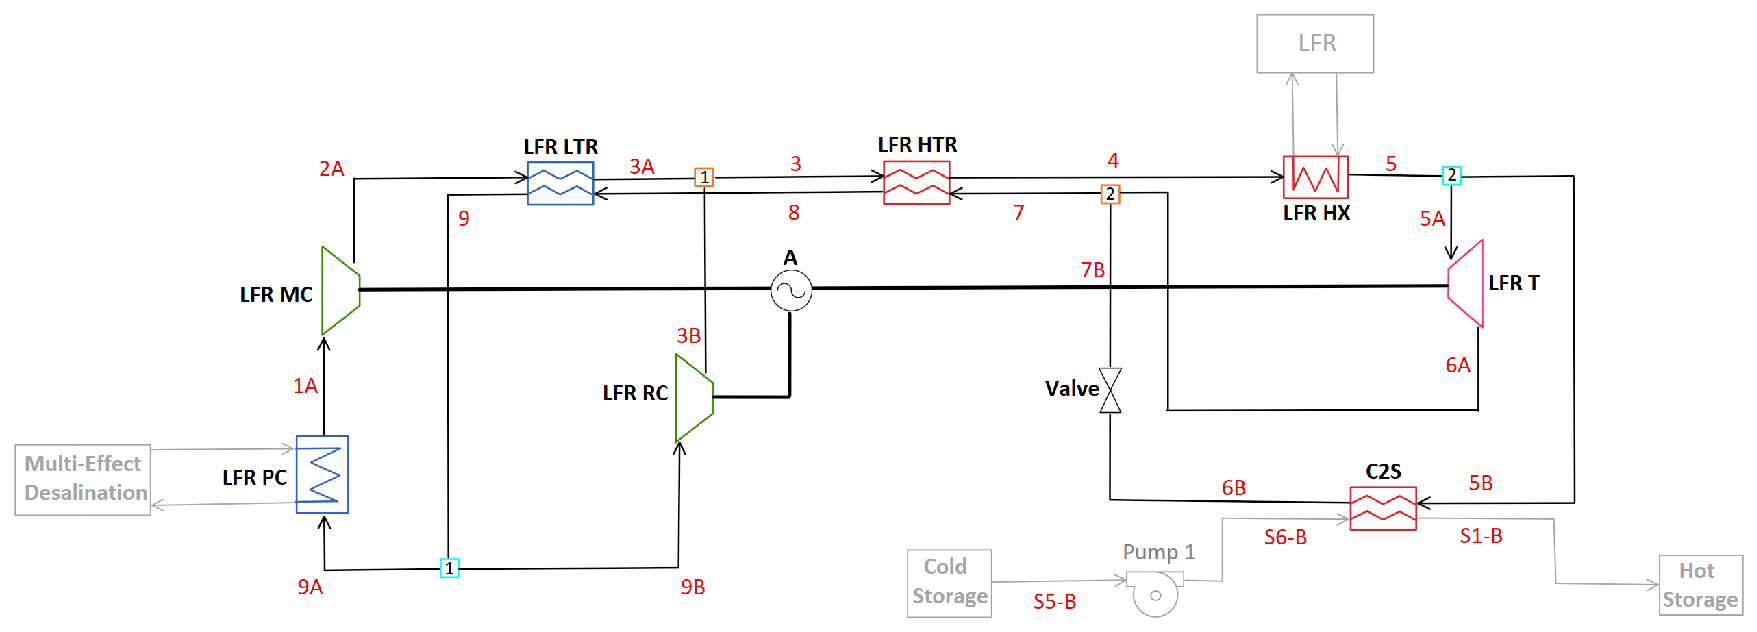
\includegraphics[width=\linewidth]{Definitions/c-lfr-par.pdf}
    \caption{Diagram for C-LFR-PAR thermal energy storage charging orientation\label{c-lfr-par}.}
\end{figure}
\begin{paracol}{2}
%\linenumbers
\switchcolumn

\vspace{-6pt}
\subsubsection{C-LFR-CIRC} 
%--------------------------------------------------------------------------------------

The full diagram for C-LFR-CIRC is shown in Figure~\ref{c-lfr-circ}.
\end{paracol}
\begin{figure}[H]
    \widefigure
    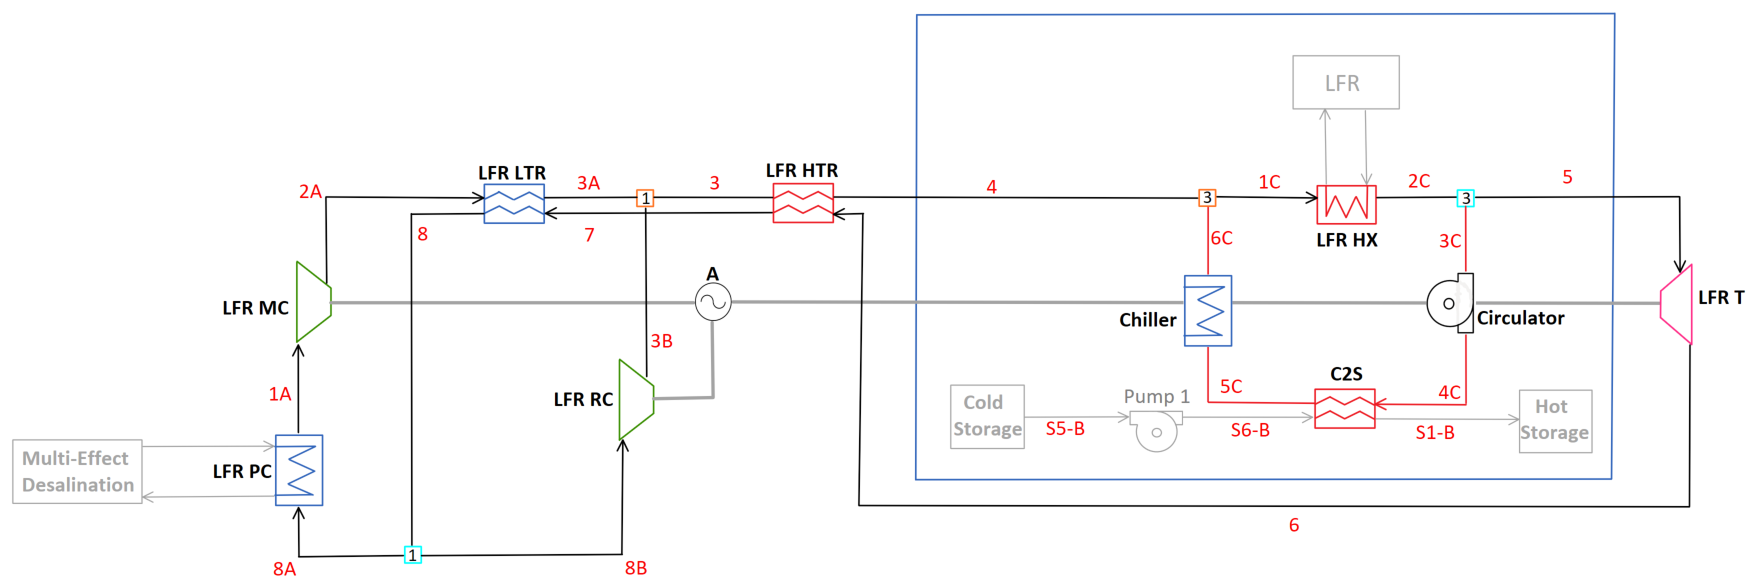
\includegraphics[width=\linewidth]{Definitions/c-lfr-circ.pdf}
    \caption{Full diagram for C-LFR-CIRC thermal energy storage charging orientation\label{c-lfr-circ}.}
\end{figure}
\begin{paracol}{2}
%\linenumbers
\switchcolumn

The charging subsection of this diagram is composed of a circulation cycle that has heat inputted through the LFR heat exchanger. A~separated circulation cycle has a loop which avoids the losses associated with compressor and turbine, therefore achieving higher heat storage efficiency than possible with full cycle operation. This subsection is encircled in blue and can be seen in Figure~\ref{c-lfr-circ-sub}.

The flow continues through a circulator which is assumed to have negligible pressure rise (i.e. there is assumed to be negligible pressure drop in this case). A~heat exchanger, C2S, extracts heat from the flow, storing the thermal energy in the hot TES for later use. Excess heat that is not extracted is then dumped into a reservoir through the chiller to bring the temperature of the flow down to LFR cool side operating temperature of $400~^{\circ}$C. Three different cold TES temperatures---$390~^{\circ}$C, $410~^{\circ}$C, and~$440~^{\circ}$C---are compared in a sensitivity~study. 

% \end{paracol}
\begin{figure}[H]
   % \widefigure
    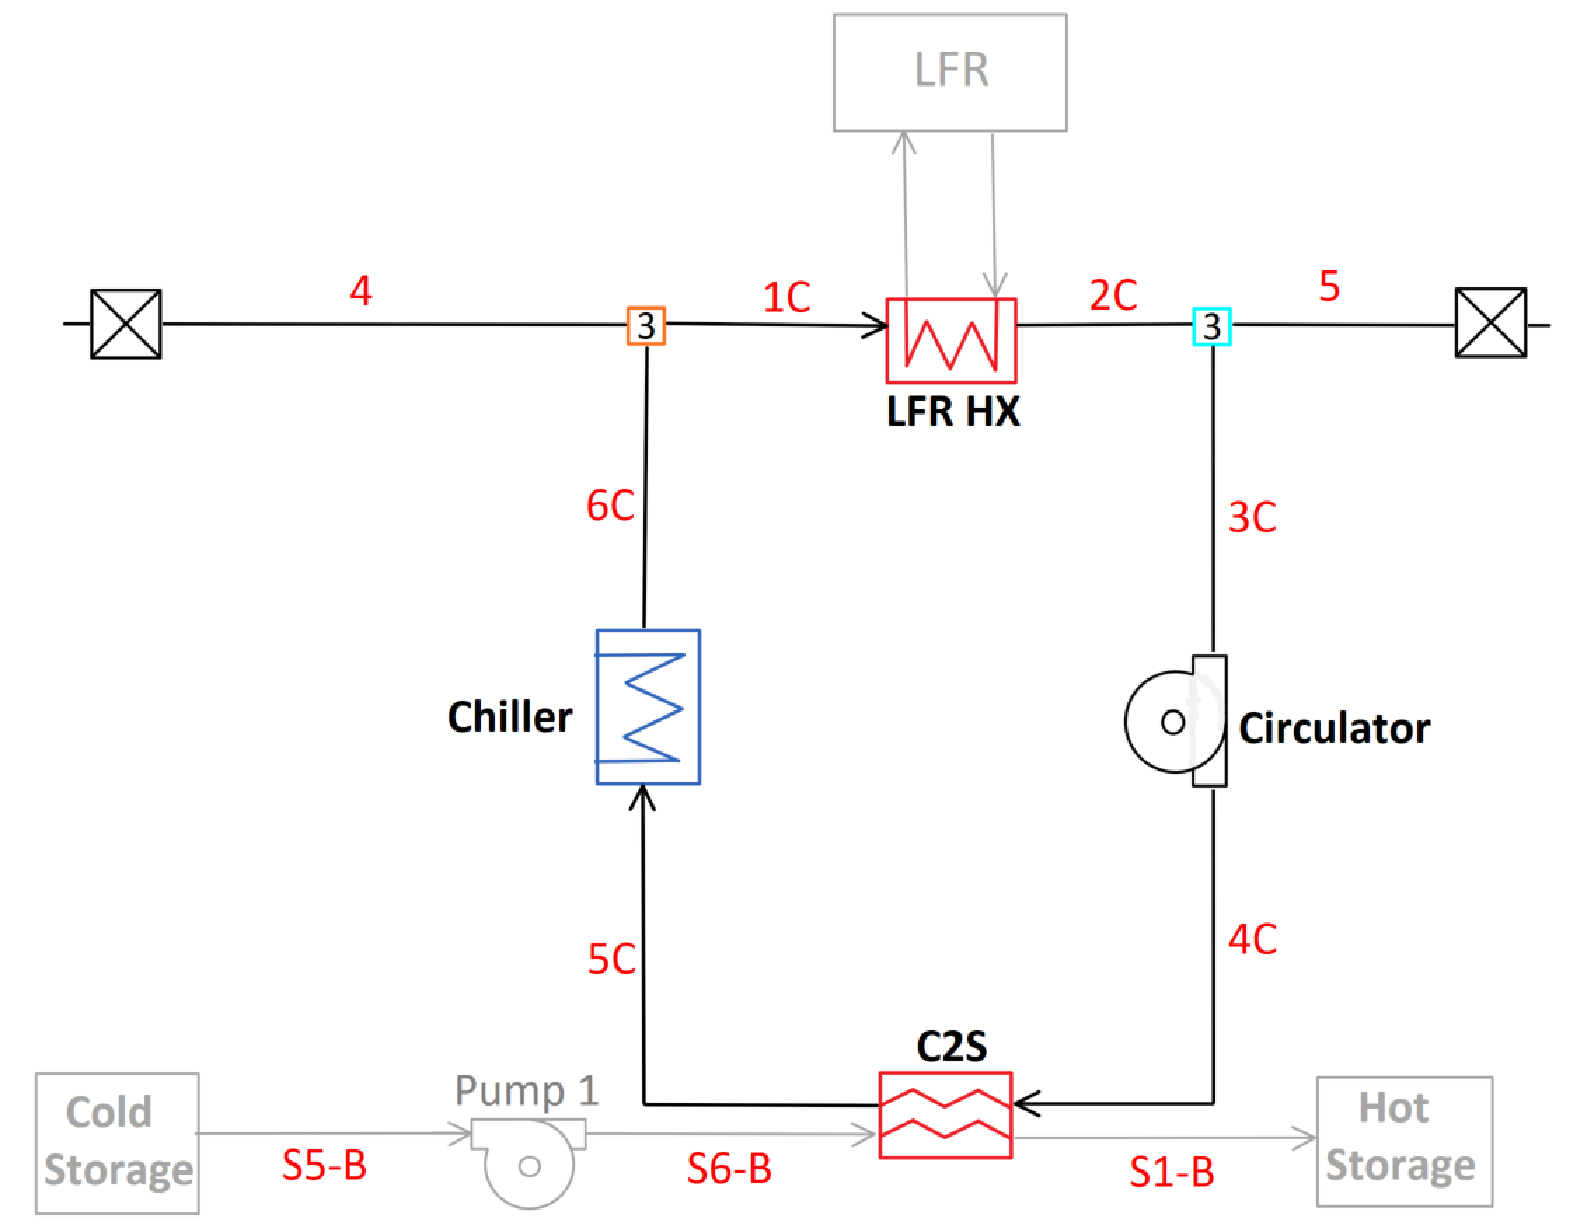
\includegraphics[width=0.7\linewidth]{Definitions/c-lfr-circ-sub.pdf}
    \caption{Diagram for C-LFR-CIRC sub-cycle thermal energy storage charging orientation\label{c-lfr-circ-sub}.}
\end{figure}
% \begin{paracol}{2}
% %\linenumbers
% \switchcolumn




%%%%%%%%%%%%%%%%%%%%%%%%%%%%%%%%%%%%%%%%%%%%%%%%%%%%%%%%%%%%%%%%%%%%%%%%%%%%%%%%%%%%%%%
\section{Results and~Discussion}

For all cycle configurations presented, with~constrained or unconstrained LFR low-temperature inlet and varied cold TES temperature, cycle and heat storage efficiencies are maximized using parametric studies on flow splitter fractions. %\replaced[comment={Source of calculations defined [4,3]}]
{All calculations were carried out using EES, with~the results}
%{These results are} 
obtained using standardized values found in \mbox{Table \ref{tab-cycle_sum}} for a more direct comparison between cycles. Presentation and discussion of the results is fulfilled in the following~section. 

\subsection{Non-Charging Cycle~Configurations}
%======================================================================================

The three non-charging cycle models have a focus on producing the highest positive alternator power to heat input, or~cycle efficiency. The~two-cycle configuration, composed of C-LFR-ON and C-CSP-ON, has independent recompression cycles with dedicated compressors, turbine, recuperators, and~pre-cooler for the LFR and CSP. C-1HTR1T-ON, with~the heat additions in parallel, and~C-2HTR3T, with~dedicated HTR for both heat additions, are cycles which incorporate the CSP and LFR in the same cycle. The~results from studies performed on these cycles are displayed in Table~\ref{tab-noncharg}. 

The calculated values reported in Table~\ref{tab-noncharg} are component power, mass flow fractions, and~counter-flow heat exchanger specifications. Columns labeled with '$C$' headers have the LFR sCO$_2$ low inlet temperature constrained to 400$~^{\circ}$C while those labeled with '$U$' are unconstrained and calculated based off a parametric study on the MC mass flow fraction. Values listed in the Cold TES Temperature row are set to values of 390$~^{\circ}$C, 410$~^{\circ}$C, or~440$~^{\circ}$C to study the effects that cold TES temperature has on cycle efficiency and to accommodate certain characteristics of cycle configurations. %\replaced[comment={Removed the conjunction 'and' in the sentence for clarity. [1,1]}]
{Cycles that do not contain the listed component omit the associated values.}
%{Cycles that do not contain the listed component and omit the associated values.} 
\clearpage 
% \mw{Check that the column breakdown and grouping is correct in what I've changed.}
\end{paracol}
\begin{specialtable}[H] 
    %[htbp]
    
    \caption{\hl{Calculated} system parameters for non-charging cycle configurations with constrained (\textit{C}) and unconstrained (\textit{U}) lead-cooled fast reactor low-end temperature.\label{tab-noncharg}}%is the Vertical line necessary?
    \resizebox{\columnwidth}{!}{
    \begin{tabular}{lc|cc|cc|ccc|ccc}
    \toprule
     &  & \multicolumn{2}{c|}{\textbf{C-LFR-ON}} & \multicolumn{2}{c|}{\textbf{C-CSP-ON}}  &	\multicolumn{3}{c|}{\textbf{C-1HTR1T-ON}}	&	\multicolumn{3}{c}{\textbf{C-2HTR3T-ON}} \\
    \textbf{Definition} & \textbf{Variable} & \textit{U} & \textit{C} & \textit{N/A} & \textit{N/A} &	\textit{U}	&	\textit{C}	&	\textit{C}	&	\textit{U}	&	\textit{C}	&	\textit{C}
    \\
    \midrule
    Cycle Efficiency (\%)	&	$\eta_{cycle}$	&	47.08	&	45.28	&	45.58	&	45.93	&	44.9	&	44.22	&	44.22	&	46.10	&	44.34	&	44.35	\\
    LFR Inlet Temperature ($~^{\circ}$C)	&	$T_{4,4C,5A}$	&	415.1	&	400	&	$\cdot$	&	$\cdot$	&	380	&	400	&	400	&	415.2	&	400	&	400	\\
    Cold TES Temperature ($~^{\circ}$C)	&	$T_{CS}$	&	$\cdot$	&	$\cdot$	&	390	&	440	&	390	&	410	&	440	&	390	&	390	&	440	\\
    Alternator Power (MW)	&	$\dot{W}_{A}$	&	447.3	&	430.2	&	339.1	&	340.6	&	763.9	&	752.3	&	752.6	&	783.7	&	753.7	&	754	\\
    PC Heat Transfer (MW)	&	$\dot{Q}_{PC}$	&	502.7	&	519.8	&	418.5	&	420.2	&	937.4	&	949.2	&	949.3	&	917.6	&	947.6	&	947.9	\\
    MC Power (MW)	&	$\dot{W}_{MC}$	&	115	&	118.9	&	95.73	&	96.13	&	214.5	&	194.8	&	194.8	&	209.9	&	216.8	&	216.9	\\
    RC Power (MW)	&	$\dot{W}_{RC}$	&	116.6	&	77.3	&	97.22	&	97.71	&	217.4	&	285.7	&	285.7	&	213.5	&	140.8	&	140.8	\\
    T1 Power (MW)	&	$\dot{W}_{T1}$	&	678.9	&	626.4	&	532.1	&	534.5	&	1196	&	1233	&	1233	&	679.3	&	626.3	&	626.3	\\
    T2 Power (MW)	&	$\dot{W}_{T2}$	&	$\cdot$	&	$\cdot$	&	$\cdot$	&	$\cdot$	&	$\cdot$	&	$\cdot$	&	$\cdot$	&	527.8	&	485	&	485.4	\\
    MC Mass Flow Fraction (-)	&	$y_{1}$	&	0.7	&	0.7844	&	0.6996	&	0.6994	&	0.7	&	0.6333	&	0.6333	&	0.6993	&	0.7846	&	0.7846	\\
    LFR Mass Flow Fraction (-)	&	$y_{2}$	&	$\cdot$	&	$\cdot$	&	$\cdot$	&	$\cdot$	&	0.4485	&	0.4928	&	0.4929	&	0.5478	&	0.5486	&	0.5484	\\
    LTR UA Value (MW/$~^{\circ}$C)	&	$UA_{LTR}$	&	54.68	&	22.84	&	45.4	&	45.53	&	102	&	91.63	&	91.64	&	134.4	&	41.56	&	41.57	\\
    LTR Capacitance Ratio (-)	&	$CR_{LTR}$	&	0.9867	&	0.8473	&	0.9858	&	0.9854	&	0.9867	&	0.9066	&	0.9066	&	0.9853	&	0.847	&	0.847	\\
    LTR Heat Transfer Rate (MW)	&	$\dot{Q}_{LTR}$	&	656.8	&	366.5	&	548.3	&	551.4	&	549.2	&	614.9	&	615.1	&	1204	&	667.1	&	667.3	\\
    LTR Effectiveness (-)	&	$\varepsilon_{LTR}$	&	0.92	&	0.8742	&	0.9201	&	0.9202	&	0.92	&	0.9485	&	0.9485	&	0.9414	&	0.8741	&	0.8741	\\
    HTR UA Value (MW/$~^{\circ}$C)	&	$UA_{HTR}$	&	48.29	&	42.71	&	34.58	&	34.72	&	78.22	&	82.3	&	82.34	&	48.32	&	42.69	&	42.69	\\
    HTR Capacitance Ratio (-)	&	$CR_{HTR}$	&	0.8657	&	0.8143	&	0.8593	&	0.8594	&	0.8595	&	0.8754	&	0.8755	&	0.8661	&	0.8142	&	0.8142	\\
    HTR Heat Transfer Rate (MW)	&	$\dot{Q}_{HTR}$	&	998.1	&	1161	&	665.4	&	667.7	&	679.2	&	742.6	&	743	&	545.7	&	636.8	&	636.6	\\
    HTR Effectiveness (-)	&	$\varepsilon_{HTR}$	&	0.9544	&	0.9627	&	0.9436	&	0.9436	&	0.9445	&	0.9441	&	0.9441	&	0.9542	&	0.9627	&	0.9627	\\
    HTR2 UA Value (MW/$~^{\circ}$C)	&	$UA_{HTR2}$	&	$\cdot$	&	$\cdot$	&	$\cdot$	&	$\cdot$	&	$\cdot$	&	$\cdot$	&	$\cdot$	&	34.29	&	31.61	&	31.63	\\
    HTR2 Capacitance Ratio (-)	&	$CR_{HTR2}$	&	$\cdot$	&	$\cdot$	&	$\cdot$	&	$\cdot$	&	$\cdot$	&	$\cdot$	&	$\cdot$	&	0.8594	&	0.8074	&	0.8074	\\
    HTR2 Heat Transfer Rate (MW)	&	$\dot{Q}_{HTR2}$	&	$\cdot$	&	$\cdot$	&	$\cdot$	&	$\cdot$	&	$\cdot$	&	$\cdot$	&	$\cdot$	&	298.1	&	363.4	&	363.8	\\
    HTR2 Effectiveness (-)	&	$\varepsilon_{HTR2}$	&	$\cdot$	&	$\cdot$	&	$\cdot$	&	$\cdot$	&	$\cdot$	&	$\cdot$	&	$\cdot$	&	0.9436	&	0.9561	&	0.9561	\\
    CSPHX UA Value (MW/$~^{\circ}$C)	&	$UA_{CSPHX}$	&	$\cdot$	&	$\cdot$	&	71.34	&	26.92	&	33.72	&	73.4	&	35.05	&	70.88	&	44.92	&	23.13	\\
    CSPHX Capacitance Ratio (-)	&	$CR_{CSPHX}$	&	$\cdot$	&	$\cdot$	&	0.9924	&	0.701	&	0.8104	&	0.9957	&	0.8034	&	0.9926	&	0.9138	&	0.6454	\\
    CSPHX Heat Transfer Rate (MW)	&	$\dot{Q}_{CSPHX}$	&	$\cdot$	&	$\cdot$	&	757.6	&	760.8	&	751.3	&	751.5	&	751.9	&	751.3	&	751.3	&	751.9	\\
    CSPHX Effectiveness (-)	&	$\varepsilon_{CSPHX}$	&	$\cdot$	&	$\cdot$	&	0.945	&	0.945	&	0.945	&	0.9381	&	0.9374	&	0.9450	&	0.9493	&	0.9493	\\
    \bottomrule
    \end{tabular}
    }
\end{specialtable}
\begin{paracol}{2}
%\linenumbers
\switchcolumn


\subsubsection{Two-Cycle Configuration: C-LFR-ON and~C-CSP-ON}

The two-cycle configuration has the CSP and LFR operating in separate recompression cycles when the focus is on electrical generation, and therefore these two cycles are analyzed individually. C-LFR-ON has the highest efficiency during unconstrained operation with a gain of 1.8 percentage points. The~unconstrained case allows for smaller temperature gradient across the LFR, an~increase in recuperator effectiveness, and~an increase in recuperator capacitance ratio, all of which reduce sources of irreversibility in the cycle~\cite{klein_nellis_2011}. Increasing the LFR sCO$_2$ inlet temperature above the design value of $400~^{\circ}$C is favorable from a cycle efficiency perspective, but~reduces the LFR thermal power. This is because the LFR mass flow rate and outlet temperature are constrained by materials properties (to limit creep, corrosion and erosion), so a lower inlet temperature implies a lower thermal power. In~principle, dropping the LFR inlet temperature further, to~as low as $340~^{\circ}$C (beyond which lead freezing becomes limiting), would further increase thermal power at the expense of cycle efficiency, so a trade-off is needed. When unconstrained, the~sCO$_2$ inlet temperature to the LFR increases by $15.1~^{\circ}$C to a value of $415.1~^{\circ}$C, increasing LFR efficiency but demanding a larger, more idealized, LFR heat~exchanger.

C-CSP-ON is not affected by constrained or unconstrained LFR sCO$_2$ inlet temperature because C2S is turned off and therefore the two cycles are not tethered during non-charging configuration. Two individual studies are conducted on the C-CSP-ON cycle cold TES temperature, one with a lower design value of $390~^{\circ}$C and another with a higher value of $440~^{\circ}$C. A~cold TES temperature of $410~^{\circ}$C is excluded since it can be presumed to have an efficiency intermediate to the $390~^{\circ}$C and $440~^{\circ}$C calculated values. Cold TES temperature is found to have a negligible effect on cycle efficiency between the two studied cases, with~the $440~^{\circ}$C case gaining 0.35 percentage points. The~component that has the largest change in values is the CSP HX with a large drop in capacitance ratio and UA value, and therefore the lower temperature of $390~^{\circ}$C for cold TES temperature is ideal, increasing the performances of the heat~exchanger. 

Combining the two-cycle efficiencies using Equation~(\ref{eq-eta-2cycle}) gives a more direct comparison to the single-cycle configurations; C-1HTR1T and C-2HTR3T. Two combined efficiencies are calculated for the two-cycle configuration combination. The~first has the highest efficiency, combining the unconstrained C-LFR-ON LFR low-temperature and C-CSP-ON $440~^{\circ}$C cold TES cases. This combined efficiency yields a value of 46.1\% (which is almost identical to the efficiency achieved by C-2HTR3T-ON shown in Table~\ref{tab-noncharg}). The~second combined configuration has a lower efficiency with favorable LFR characteristics and solar salt mass flow rate. This combination has the constrained C-LFR-ON LFR low-temperature and C-CSP-ON $390~^{\circ}$C cold TES cases with a combined efficiency of 45.1\%. 


\subsubsection{C-1HTR1T-ON}
The single-cycle configuration, C-1HTR1T-ON, has the CSP and LFR heat additions in parallel causing identical inlet conditions. Due to the $10~^{\circ}$C approach temperature, the~identical inlet conditions lead to a lower bound of $410~^{\circ}$C on the cold TES temperature when the sCO$_2$ LFR inlet temperature is constrained to $400~^{\circ}$C. A~supplementary $440~^{\circ}$C cold TES study is run to test the effects that higher temperature storage has on cycle efficiency. Raising the temperature of the cold TES from $410~^{\circ}$C to $440~^{\circ}$C has no effect on cycle efficiency but did raise the solar salt mass flow rate to accommodate for the lower temperature difference across the CSP HX hot side. Increasing the solar salt mass flow rate requires more storage for the same CSP heat input, a~reduction in dispatchability, and~larger pumps, increasing the cost of the system. Therefore, a~lower cold TES temperature is desirable. Without~the constraint on the sCO$_2$ LFR inlet temperature, a~study is additionally conducted with cold TES temperature set to $390~^{\circ}$C. Of~these three sensitivity studies, the~cycle that yielded the highest efficiency is the unconstrained, $390~^{\circ}$C cold TES with an efficiency gain of 0.68 percentage points over the constrained cases. The~high temperature difference between the hot and cold TES reduces the mass flow rate of solar salt and subsequent cost of system components. The~sCO$_2$ LFR inlet temperature for the $390~^{\circ}$C cold TES study is $380~^{\circ}$C, which increases the performance of the LFR heat exchanger as well as allowing for a higher core~power. 

\subsubsection{C-2HTR3T-ON}
C-2HTR3T-ON has dedicated recuperators and turbines for the LFR and CSP, allowing for independent inlet temperatures. Three studies are conducted on this cycle with two being constrained and one unconstrained sCO$_2$ LFR inlet conditions. The~constrained studies have cold TES temperatures of $390~^{\circ}$C and $440^{\circ}$, both of which have negligible efficiency differences. Similarly to the studies performed on C-1HTR1T-ON, the~$440~^{\circ}$C cold TES temperature case has a larger mass flow rate of solar salt and therefore increases component cost. The~$390~^{\circ}$C unconstrained study has the highest efficiency with a value of 46.10\%, 1.76 percentage points more than the constrained cases. Additionally, the~sCO$_2$ LFR inlet temperature is $415.2~^{\circ}$C, $15.2~^{\circ}$C more than constrained cases, causing heat exchanger parameters to be less than ideal but increasing LFR~efficiency.

\subsection{Thermal Energy Storage Charging~Techniques}

When the focus of the cycles is thermal storage for later use, the~LFR charges the hot TES through the C2S heat exchanger. Studies performed on the charging techniques have constrained sCO$_2$ LFR inlet temperatures to $400~^{\circ}$C with set values of cold TES temperature of $390~^{\circ}$C, $410~^{\circ}$C, or~$440~^{\circ}$C. The~two charging techniques which run the full recompression cycle are C-LFR-PRE, with~the turbine before the heat extraction, and~C-LFR-PAR, with~heat extraction in parallel to the turbine. The~third charging technique, C-LFR-CIRC, has a dedicated circulation loop and additional chiller and circulator pump to avoid losses associated with the compressors and turbines. The~results are presented in Table~\ref{tab-charg}.  


% \end{paracol}

\begin{specialtable}[H]  
    %[htbp]
    \caption{\hl{Calculated} system parameters for charging cycle configurations. All cases were evaluated with constrained (\textit{C}) lead-cooled fast reactor low-end temperature.\label{tab-charg}}%is the Vertical line necessary?
    \resizebox{\columnwidth}{!}{
        \begin{tabular}{lc|c|cc|ccc}
            \toprule
            &  & \textbf{C-LFR-PRE} & \multicolumn{2}{c|}{\textbf{C-LFR-PAR}}  &	\multicolumn{3}{c}{\textbf{C-LFR-CIRC}} \\
            \textbf{Definition} & \textbf{Variable} & \textit{C} & \textit{C} & \textit{C} & \textit{C} &	\textit{C}	&	\textit{C}\\
            \midrule
            Cold TES Temperature ($~^{\circ}$C)	&	$T_{CS}$	&	390	&	390	&	440	&	390	&	410	&	440	\\
            LFR Inlet Temperature ($~^{\circ}$C)	&	$T_{4,1C}$	&	400	&	400	&	400	&	400	&	400	&	400	\\
            Heat Storage Efficiency (\%)	&	$\eta_{heatstorage}$	&	34.53	&	45.30	&	45.30	&	99.92	&	89.66	&	74.29	\\
            Alternator Power (MW)	&	$\dot{W}_{A}$	&	0	&	0	&	0	&	$\cdot$	&	$\cdot$	&	$\cdot$	\\
            PC Heat Transfer (MW)	&	$\dot{Q}_{PC}$	&	622	&	519.6	&	519.6	&	$\cdot$	&	$\cdot$	&	$\cdot$	\\
            MC Power (MW)	&	$\dot{W}_{MC}$	&	142.3	&	118.9	&	118.9	&	$\cdot$	&	$\cdot$	&	$\cdot$	\\
            RC Power (MW)	&	$\dot{W}_{RC}$	&	21.89	&	77.28	&	77.28	&	$\cdot$	&	$\cdot$	&	$\cdot$	\\
            Turbine Power (MW)	&	$\dot{W}_{T}$	&	164.2	&	196.2	&	196.2	&	$\cdot$	&	$\cdot$	&	$\cdot$	\\
            Chiller Heat Transfer (MW)	&	$\dot{Q}_{chill}$	&	$\cdot$	&	$\cdot$	&	$\cdot$	&	0.7245	&	98.25	&	244.2	\\
            MC Mass Flow Fraction (-)	&	$y_{1}$	&	0.9389	&	0.7844	&	0.7844	&	$\cdot$	&	$\cdot$	&	$\cdot$	\\
            C2S Mass Flow Fraction (-)	&	$y_{2}$	&	$\cdot$	&	0.6867	&	0.6867	&	$\cdot$	&	$\cdot$	&	$\cdot$	\\
            Valve Mass Flow Fraction (-)	&	$y_{5}$	&	0.7378	&	$\cdot$	&	$\cdot$	&	$\cdot$	&	$\cdot$	&	$\cdot$	\\
            LTR UA Value (MW/$~^{\circ}$C)	&	$UA_{LTR}$	&	6.99	&	22.83	&	22.83	&	$\cdot$	&	$\cdot$	&	$\cdot$	\\
            LTR Capacitance Ratio (-)	&	$CR_{LTR}$	&	0.6754	&	0.8473	&	0.8743	&	$\cdot$	&	$\cdot$	&	$\cdot$	\\
            LTR Heat Transfer Rate (MW)	&	$\dot{Q}_{LTR}$	&	93.05	&	366.4	&	366.4	&	$\cdot$	&	$\cdot$	&	$\cdot$	\\
            LTR Effectiveness (-)	&	$\varepsilon_{LTR}$	&	0.6384	&	0.8742	&	0.8742	&	$\cdot$	&	$\cdot$	&	$\cdot$	\\
            HTR UA Value (MW/$~^{\circ}$C)	&	$UA_{HTR}$	&	41.69	&	42.69	&	42.69	&	$\cdot$	&	$\cdot$	&	$\cdot$	\\
            HTR Capacitance Ratio (-)	&	$CR_{HTR}$	&	0.7531	&	0.8143	&	0.8143	&	$\cdot$	&	$\cdot$	&	$\cdot$	\\
            HTR Heat Transfer Rate (MW)	&	$\dot{Q}_{HTR}$	&	1567	&	1160	&	1160	&	$\cdot$	&	$\cdot$	&	$\cdot$	\\
            HTR Effectiveness (-)	&	$\varepsilon_{HTR}$	&	0.9695	&	0.9627	&	0.9627	&	$\cdot$	&	$\cdot$	&	$\cdot$	\\
            C2S UA Value (MW/$~^{\circ}$C)	&	$UA_{C2S}$	&	9.04	&	8.037	&	14.24	&	48.29	&	43.16	&	35.63	\\
            C2S Capacitance Ratio (-)	&	$CR_{C2S}$	&	0.4735	&	0.7556	&	0.9339	&	0.8755	&	0.8599	&	0.8294	\\
            C2S Heat Transfer Rate (MW)	&	$\dot{Q}_{C2S}$	&	328	&	430.4	&	430.4	&	949.3	&	851.8	&	705.8	\\
            C2S Effectiveness (-)	&	$\varepsilon_{C2S}$	&	0.9368	&	0.8275	&	0.8307	&	0.9511	&	0.9459	&	0.9355	\\
            C2S Approach Temperature ($~^{\circ}$C)	&	$\delta_{C2S}$	&	10	&	35	&	26.27	&	10	&	10	&	10	\\
            \bottomrule
        \end{tabular}
        }
    \end{specialtable}
    % \begin{paracol}{2}
        % %\linenumbers
        % \switchcolumn
        
\subsubsection{C-LFR-PRE}
The TES charging technique with the turbine prior to the C2S heat exchanger, C-LFR-PRE, requires the temperature of the C2S inlet to be high enough to charge the hot TES. The~hot TES is at a temperature of 560$~^{\circ}$C, with~a 10$~^{\circ}$C approach temperature, and therefore the inlet temperature to C2S is required to be at least 570$~^{\circ}$C. In~cases where the turbine outlet temperature is less than 570$~^{\circ}$C, a~isenthalpic valve bypasses flow from the high-temperature turbine inlet and mixes with the low-temperature turbine outlet raising the temperature prior to the C2S heat exchanger. For~the C-LFR-PRE configuration to be viable, it requires a larger temperature than the set LFR HX outlet temperature of 595$~^{\circ}$C. With~this low of a LFR outlet temperature, \hl{73.8}\% of the flow is redirected around the turbine to raise the temperature prior to C2S. As~the temperature of the hot TES is raised above a value of 540$~^{\circ}$C, the~amount of flow around the turbine approaches 100\% and balancing the turbine power to compressor power is infeasible. The~temperature in the hot TES is therefore set to a lower value of 540$~^{\circ}$C to allow for operation of this cycle. With~heat storage efficiency maximized, \hl{93.9}\% of the flow is sent to the main compressor, rejecting 622 MW of heat out of the cycle through the precooler. This amount of rejected heat is reflected in a heat storage efficiency of \hl{34.5}\%, the~lowest of all tested TES charging~configurations.

\subsubsection{C-LFR-PAR}

To test the effects of splitting flow prior to the turbine, a~parallel configuration C-LFR-PAR is studied. To~reduce the pressure from 28.8 MPa to 8.8 MPa, an~isenthalpic valve is required after heat is extracted for storage through C2S. With~this configuration two different values for cold TES are studied, one with a cold TES storage of $390~^{\circ}$C the other with a temperature of $440~^{\circ}$C. A~noteworthy difference for this cycle is the C2S approach temperature is not set to $10~^{\circ}$C. Defining the approach temperature as $10~^{\circ}$C causes the energy balance governing combiner 2 to be over constrained. Therefore, this value is free and calculated to be $35~^{\circ}$C for the $390~^{\circ}$C case and $26.3~^{\circ}$C for the $440~^{\circ}$C case. Both of these different temperature cold TES studies do not change the cycle parameters because, as~seen in C-1HTR1T-ON and C-2HTR3T-ON, the~solar salt mass flow rate adjusts to accommodate for the temperature difference. The~higher cold TES temperature of $440~^{\circ}$C causes the mass flow rate in the CSP to increase by approximately 650 kg/s. Increasing the mass flow rate has a higher demand on system components but in this situation it allows for the salt to be charged at a higher rate, increasing the storage capabilities. Both cycles have a heat storage efficiency of \hl{45.3}\%.

\subsubsection{C-LFR-CIRC}

C-LFR-CIRC is a thermal energy storage charging technique which does not suffer from significant losses associated with turbines, compressors, and~heat exchangers. The~separate recirculation cycle is modeled extracting heat directly from the LFR, passes the high-temperature mass flow through a circulator, exchanges the heat into the hot TES through C2S, then removes heat in a chiller to bring the temperature of the flow down to the inlet temperature of the LFR, ideally $400~^{\circ}$C. This is the most adoptable TES charging technique with a wide range of possible TES charging temperatures while transferring a majority of the heat from the LFR into the hot TES. Multiple temperatures for the cold TES are studied; $390~^{\circ}$C, $410~^{\circ}$C, and~$440~^{\circ}$C. Of~these three temperatures, the~highest efficiency is a cold TES temperature of $390^{\circ}$ with a heat storage efficiency of 100\% (not accounting for pressure drop losses, which will be small). The~heat storage efficiency reduces as the temperature of the cold TES is increased; the $410~^{\circ}$C case has an efficiency of 90\% while the $440~^{\circ}$C case has an efficiency of 74\%. This reduction in efficiency is due to the inlet temperature condition on the LFR, the~higher the temperature of the cold TES the higher the temperature of the C2S outlet and therefore more heat is being extracted through the chiller to bring the flow temperature down to the LFR inlet~temperature. 

There is an interaction between the temperatures selected here and the non-charging cycle configuration. For~C-LFR-CIRC, the~highest efficiencies are achieved when the cold TES temperature is $10~^{\circ}$C less than the inlet to the LFR, this is due to the approach temperature on the C2S heat exchanger. If~the sCO$_2$ LFR inlet temperature is constrained to $400~^{\circ}$C, then the desired cold TES temperature is $390~^{\circ}$C to allow for the approach temperature. If~the cold TES is at a higher temperature, then the chiller is needed. This then implies that the sCO$_2$ inlet temperature in the salt-to-sCO$_2$ heat exchanger is  $380~^{\circ}$C. From~the results of the previous section, this is clearly achievable for the C-2HTR3T-ON configuration and the separate cycle configuration, but~for the C-1HTR1T-ON configuration the LFR and CSP inlet temperatures are constrained to be the same. In~this case, the~LFR and CSP inlet temperatures would then be $400~^{\circ}$C, implying a cold TES temperature of  $410~^{\circ}$C and hence a 90\% heat storage efficiency with a requirement for a~chiller.


%%%%%%%%%%%%%%%%%%%%%%%%%%%%%%%%%%%%%%%%%%%%%%%%%%%%%%%%%%%%%%%%%%%%%%%%%%%%%%%%%%%%%%%
\section{Conclusions}

This paper analyzed contending sCO$_2$ Brayton cycle configurations for complimentary CSP and LFR cycles with non-charging cycle configurations focusing on electrical generation. An~additional operating mode, hot TES charging, is considered where the CSP hot TES is charged by the LFR when grid demand is low. This operating mode positions the heat extraction point at different locations around the turbine in a sCO$_2$ Brayton recompression cycle. The~performance parameters that are used for comparison of the cycles are cycle efficiency when the cycle is producing electricity and heat storage efficiency when the focus is on energy storage for later use in the charging mode. These efficiencies are maximized using flow splitter values at different values of cold TES temperature and constrained or unconstrained sCO$_2$ inlet LFR temperature. The~conclusions drawn in this paper are as follows:

\textit{\hl{Non-charging configurations:}}%we recomended it can be format as~subsection
\begin{itemize}
    \item	Two-cycle configuration C-LFR-ON and C-CSP-ON: Offers the highest cycle efficiency because of the freedom of the two cycles to operate independently when generating electrical power. The~cycles individually are simple recompression but there is a lack of component synergies.
    \item	C-1HTR1T-ON: Single-cycle configuration that is the least complex, and therefore cost efficient and compact, with~heat additions from the CSP and LFR in parallel. With~both CSP and LFR discharging, combined cycle efficiency is reduced by ~0.8 percentage points compared to the two-cycle configuration. 
    \item   C-2HTR3T-ON: Single-cycle configuration that has dedicated turbines and HTRs for the LFR and CSP. This cycle makes a compromise between complexity with reduced cycle component redundancy, flexibility for dissimilar inlet temperatures on the CSP and LFR inlet, and~median efficiency. The~efficiency is only marginally higher than C-1HTR1T-ON, but~heat storage efficiency when using the LFR to charge the salt is improved due to flexibility on setting the CSP and LFR inlet temperatures. As~the additional turbines are likely present in practice anyway, this cycle is not anticipated to significantly increase cost and complexity over C-1HTR1T-ON. The~relative merits of C-2HTR3T-ON and C-1HTR1T-ON are therefore similar. It is noted that for the unconstrained case C-2HTR3T achieves almost identical performance to the two-cycle configuration, with~an efficiency of 46.1\%, and~hence the drop in performance relative to using separate cycles is attributable to the constraint on LFR inlet temperature being more limiting.
\end{itemize}

\textit{\hl{Thermal energy storage charging techniques:}}
\begin{itemize}
    \item    C-LFR-POST: Charging technique with the turbine subsequent to C2S heat exchanger. Infeasible due to lower thermodynamic efficiency. 
    \item	C-LFR-PRE: Charging technique with the turbine prior to C2S heat exchanger with a valve that bypasses the turbine, demands a high outlet temperature for the LFR to be effective. Due to LFR outlet temperature limitations, this configuration has the next lowest heat storage efficiency.
    \item	C-LFR-PAR: Charging technique that splits the flow directly after the LFR with the turbine and C2S heat exchanger in parallel. The~heat storage efficiency is higher than C-LFR-PRE.
    \item   C-LFR-CIRC: Flexible technique with a heat storage efficiency being highly dependent on cold TES temperature and LFR inlet temperature. Able to achieve heat storage efficiency to near 100\% by eliminating losses associated with the turbines and compressors. For~C-1HTR1T-ON, the~heat storage efficiency is limit to 90\% because the inlet temperatures to the LFR and CSP are constrained to be the same. The~additional chiller and circulator components in the dedicated circulation loop increase complexity and cost. 
\end{itemize}

C-LFR-PAR and C-LFR-CIRC are therefore options going forward, with~a trade-off between heat storage efficiency and component costs, with~the performance of C-LFR-CIRC also depending on the choice of charging~configuration.

The cycle configurations with the listed conclusions can be used as reference for future cycle design and proof of concept considerations. Further studies and cycle analysis must be performed before these cycles are used for implementation into a physical plant. 
\vspace{6pt} 

\authorcontributions{Conceptualization, B.L., M.W., C.S. and T.N.; methodology, B.W., M.W., C.S., T.N. and B.L.; software, B.W.; validation, B.L. and M.W.; formal analysis, B.W.; investigation, B.W.; resources, M.W. and B.L.; data curation, B.W.; writing---original draft preparation, B.W.; writing---review and editing, B.L., M.W. and T.N.; visualization, B.W.; supervision, M.W. and B.L.; project administration, B.L.; funding acquisition, B.L., M.W., C.S. and T.N. All authors have read and agreed to the published version of the~manuscript.}

\funding{This work was supported by funding received from the DOE Office of Nuclear Energy’s Nuclear Energy University Program under contract number~DE-NE0008988. }

% \institutionalreview{\hl{x}}%In this section, please add the Institutional Review Board Statement and approval number for studies involving humans or animals. Please note that the Editorial Office might ask you for further information. Please add ``The study was conducted according to the guidelines of the Declaration of Helsinki, and~approved by the Institutional Review Board (or Ethics Committee) of NAME OF INSTITUTE (protocol code XXX and date of approval).'' OR ``Ethical review and approval were waived for this study, due to REASON (please provide a detailed justification).'' OR ``Not applicable'' for studies not involving humans or animals. You might also choose to exclude this statement if the study did not involve humans or~animals.

 %\informedconsent{\hl{x}}%Any research article describing a study involving humans should contain this statement. Please add ``Informed consent was obtained from all subjects involved in the study.'' OR ``Patient consent was waived due to REASON (please provide a detailed justification).'' OR ``Not applicable'' for studies not involving humans. You might also choose to exclude this statement if the study did not involve~humans.

% Written informed consent for publication must be obtained from participating patients who can be identified (including by the patients themselves). Please state ``Written informed consent has been obtained from the patient(s) to publish this paper'' if applicable.

\dataavailability{Supporting data for this study is available on request.} 

\acknowledgments{We would like to thank Josh McTigue (NREL) for useful technical discussions on the development of the cycle configurations.}

\conflictsofinterest{The authors declare no conflict of interest. The~funders had no role in the design of the study; in the collection, analyses, or~interpretation of data; in the writing of the manuscript, or~in the decision to publish the~results'.} 

%% Optional
% \sampleavailability{Samples of the compounds ... are available from the authors.}
%% Optional
\abbreviations{Nomenclature}{
The following abbreviations and variables are used in this manuscript:\\

\noindent 
\begin{tabular}{@{}ll}
\textbf{Abbreviations}\\
A & Alternator\\
CSP & Concentrating solar power\\
C2S & sCO$_2$-to-Salt heat exchanger\\
EES & Engineering Equation Solver\\
HTR & High-temperature recuperator\\
HX & Heat exchanger\\
LFR & Lead-fast reactor\\
LTR & Low-temperature recuperator\\
MC & Main compressor\\
NREL & National Renewable Energy Laboratory\\
P & Pump\\
PC & Pre-cooler\\
RC & Re-compressor\\
sCO$_2$ & Supercritical carbon dioxide\\
T & Turbine\\
TES & Thermal energy storage\\

 \\
\end{tabular}


\noindent 
\begin{tabular}{@{}ll}
\textbf{Variables [Units]}\\
$CR$ & Capacitance ratio [-]\\
$\dot{C}$ & Capacitance rate [MW/$~^{\circ}$C]\\
$\Delta$ & Temperature difference [$~^{\circ}$C]\\
$\delta$ & Approach temperature of heat exchanger [$~^{\circ}$C]\\
$\varepsilon$ & Effectiveness of heat exchanger [-]\\
$\eta$ & Isentropic efficiency [-]\\
$h$ & Enthalpy [J/kg]\\
$\dot{m}$ & Mass flow rate [kg/s]\\
$NTU$ & Number of transfer units [-]\\
$P$ & Pressure [MPa]\\
$\dot{Q}$ & Heat transfer rate [W]\\
$T$ & Temperature [$~^{\circ}$C]\\
$UA$ & Conductivity of heat exchanger [MW/$~^{\circ}$C]\\
$v$ & Volumetric flow rate [$m^3$/kg]\\
$\dot{W}$ & Power [MW]\\
$y$ & Splitter fraction [-]\\
\end{tabular}%
}


% overleaf.com/learn/latex/Code_listing
% \begin{lstlisting}[language=Python]
%     #My ees file
%     def myfunc():
%         return x
%     x = y

%     f = 8*y^2
% \end{lstlisting}


% % ------- new file

% \newcommand{\myeqnone}{%
% a^2 + b^2 = c^2
% }

% %---- back to the main file
% \begin{equation}
%     \myeqnone
%     \label{myeqnonelabel}
% \end{equation}

\end{paracol}



%%%%%%%%%%%%%%%%%%%%%%%%%%%%%%%%%%%%%%%%%%%%%%%%%%%%%%%%%%%%%%%%%%%%%%%%%%%%%%%%%%%%%%%
%\section{how to use}

%\subsection{Subsection}
%Citing a journal paper~\cite{wagner2017optimization} . Now citing a book reference~\cite{blair2005sam} or other reference types~\cite{hirsch2011standardization}. \cite{nellis_klein_2008}
%\subsubsection{Subsubsection}

%Bulleted lists look like this:
%\begin{itemize}
%\item	First bullet;
%\item	Second bullet;
%\item	Third bullet.
%\end{itemize}

%Numbered lists can be added as follows:
%\begin{enumerate}
%\item	First item; 
%\item	Second item;
%\item	Third item.
%\end{enumerate}

%The text continues here. 

%\subsection{Figures, Tables and Schemes}

%All figures and tables should be cited in the main text as Figure~\ref{fig1}, Table~\ref{tab1}, etc.

%\begin{figure}[H]
%
\includegraphics[width=10.5 cm]{Definitions/logo-mdpi}
%\caption{This is a figure. Schemes follow the same formatting. If there are multiple panels, they should be listed as: (\textbf{a}) Description of what is contained in the first panel. (\textbf{b}) Description of what is contained in the second panel. Figures should be placed in the main text near to the first time they are cited. A caption on a single line should be centered.\label{fig1}}
%\end{figure}   

% The MDPI table float is called specialtable
%\begin{specialtable}[htbp] 
%\caption{This is a table caption. Tables should be placed in the main text near to the first time they are~cited.\label{tab1}}
%%% \tablesize{} %% You can specify the fontsize here, e.g.,~\tablesize{\footnotesize}. If commented out \small will be used.
%\begin{tabular}{ccc}
%\toprule
%\textbf{Title 1}	& \textbf{Title 2}	& \textbf{Title 3}\\
%\midrule
%Entry 1		& Data			& Data\\
%Entry 2		& Data			& Data\\
%\bottomrule
%\end{tabular}
%\end{specialtable}

%\begin{listing}[H]
%\caption{Title of the listing}
%\rule{\columnwidth}{1pt}
%\raggedright Text of the listing. In font size footnotesize, small, or normalsize. Preferred format: left aligned and single spaced. Preferred border format: top border line and bottom border line.
%\rule{\columnwidth}{1pt}
%\end{listing}

%\subsection{Formatting of Mathematical Components}

%This is the example 1 of equation:
%\begin{equation}
%a = 1,
%\end{equation}

%the text following an equation need not be a new paragraph. Please punctuate equations as regular text.
%% If the documentclass option "submit" is chosen, please insert a blank line before and after any math environment (equation and eqnarray environments). This ensures correct linenumbering. The blank line should be removed when the documentclass option is changed to "accept" because the text following an equation should not be a new paragraph.

%This is the example 2 of equation:
%\end{paracol}
%\nointerlineskip
%\begin{eqnarray}
%a &=& b + c + d + e + f + g + h + i + j + k + l\nonumber \\
% &+& m + n + o + p + q + r + s + t + u + v + w + x + y + z %\nonumber
%\end{eqnarray}

% Example of a figure that spans the whole page width (the commands \widefigure and \begin{paracol}{2}, %\linenumbers, and\switchcolumn need to be present). The same concept works for tables, too.
%\begin{figure}[H]	
%\widefigure
%
\includegraphics[width=15 cm]{Definitions/logo-mdpi}
%\caption{This is a wide figure.\label{fig2}}
%\end{figure} 





%\begin{paracol}{2}
%%\linenumbers
%\switchcolumn
%Please punctuate equations as regular text. Theorem-type environments (including propositions, lemmas, corollaries etc.) can be formatted as follows:
%% Example of a theorem:
%\begin{Theorem}
%Example text of a theorem.
%\end{Theorem}

%The text continues here. Proofs must be formatted as follows:

%% Example of a proof:
%\begin{proof}[Proof of Theorem 1]
%Text of the proof. Note that the phrase ``of Theorem 1'' is optional if it is clear which theorem is being referred to.
%\end{proof}
%The text continues here.

%\end{paracol}




%%%%%%%%%%%%%%%%%%%%%%%%%%%%%%%%%%%%%%%%%%
% \setcounter{section}{-1} %% Remove this when starting to work on the template.
% \section{How to Use this Template}

% The template details the sections that can be used in a manuscript. Note that the order and names of article sections may differ from the requirements of the journal (e.g., the positioning of the Materials and Methods section). Please check the instructions on the authors' page of the journal to verify the correct order and names. For any questions, please contact the editorial office of the journal or support@mdpi.com. For LaTeX-related questions please contact latex@mdpi.com.
% %The order of the section titles is: Introduction, Materials and Methods, Results, Discussion, Conclusions for these journals: aerospace,algorithms,antibodies,antioxidants,atmosphere,axioms,biomedicines,carbon,crystals,designs,diagnostics,environments,fermentation,fluids,forests,fractalfract,informatics,information,inventions,jfmk,jrfm,lubricants,neonatalscreening,neuroglia,particles,pharmaceutics,polymers,processes,technologies,viruses,vision

% \section{Introduction}

% The introduction should briefly place the study in a broad context and highlight why it is important. It should define the purpose of the work and its significance. The current state of the research field should be reviewed carefully and key publications cited. Please highlight controversial and diverging hypotheses when necessary. Finally, briefly mention the main aim of the work and highlight the principal conclusions. As far as possible, please keep the introduction comprehensible to scientists outside your particular field of research. Citing a journal paper~\cite{ref-journal}. Now citing a book reference~\cite{ref-book1,ref-book2} or other reference types~\cite{ref-unpublish,ref-communication,ref-proceeding}. Please use the command \citep{ref-thesis,ref-url} for the following MDPI journals, which use author--date citation: Administrative Sciences, Arts, Econometrics, Economies, Genealogy, Histories, Humanities, IJFS, Journal of Intelligence, Journalism and Media, JRFM, Languages, Laws, Religions, Risks, Social Sciences.
 
% %%%%%%%%%%%%%%%%%%%%%%%%%%%%%%%%%%%%%%%%%%
% \section{Materials and Methods}

% Materials and Methods should be described with sufficient details to allow others to replicate and build on published results. Please note that publication of your manuscript implicates that you must make all materials, data, computer code, and protocols associated with the publication available to readers. Please disclose at the submission stage any restrictions on the availability of materials or information. New methods and protocols should be described in detail while well-established methods can be briefly described and appropriately cited.

% Research manuscripts reporting large datasets that are deposited in a publicly avail-able database should specify where the data have been deposited and provide the relevant accession numbers. If the accession numbers have not yet been obtained at the time of submission, please state that they will be provided during review. They must be provided prior to publication.

% Interventionary studies involving animals or humans, and other studies require ethical approval must list the authority that provided approval and the corresponding ethical approval code.
% \begin{quote}
% This is an example of a quote.
% \end{quote}

% %%%%%%%%%%%%%%%%%%%%%%%%%%%%%%%%%%%%%%%%%%
% \section{Results}

% This section may be divided by subheadings. It should provide a concise and precise description of the experimental results, their interpretation as well as the experimental conclusions that can be drawn.
% \subsection{Subsection}
% \subsubsection{Subsubsection}

% Bulleted lists look like this:
% \begin{itemize}
% \item	First bullet;
% \item	Second bullet;
% \item	Third bullet.
% \end{itemize}

% Numbered lists can be added as follows:
% \begin{enumerate}
% \item	First item; 
% \item	Second item;
% \item	Third item.
% \end{enumerate}

% The text continues here. 

% \subsection{Figures, Tables and Schemes}

% All figures and tables should be cited in the main text as Figure~\ref{fig1}, Table~\ref{tab1}, etc.

% \begin{figure}[H]
% 
\includegraphics[width=10.5 cm]{Definitions/logo-mdpi}
% \caption{This is a figure. Schemes follow the same formatting. If there are multiple panels, they should be listed as: (\textbf{a}) Description of what is contained in the first panel. (\textbf{b}) Description of what is contained in the second panel. Figures should be placed in the main text near to the first time they are cited. A caption on a single line should be centered.\label{fig1}}
% \end{figure}   

% % The MDPI table float is called specialtable
% \begin{specialtable}[H] 
% \caption{This is a table caption. Tables should be placed in the main text near to the first time they are~cited.\label{tab1}}
% %%% \tablesize{} %% You can specify the fontsize here, e.g.,~\tablesize{\footnotesize}. If commented out \small will be used.
% \begin{tabular}{ccc}
% \toprule
% \textbf{Title 1}	& \textbf{Title 2}	& \textbf{Title 3}\\
% \midrule
% Entry 1		& Data			& Data\\
% Entry 2		& Data			& Data\\
% \bottomrule
% \end{tabular}
% \end{specialtable}

% %\begin{listing}[H]
% %\caption{Title of the listing}
% %\rule{\columnwidth}{1pt}
% %\raggedright Text of the listing. In font size footnotesize, small, or normalsize. Preferred format: left aligned and single spaced. Preferred border format: top border line and bottom border line.
% %\rule{\columnwidth}{1pt}
% %\end{listing}

% Text.

% Text.

% \subsection{Formatting of Mathematical Components}

% This is the example 1 of equation:
% \begin{equation}
% a = 1,
% \end{equation}
% the text following an equation need not be a new paragraph. Please punctuate equations as regular text.
% %% If the documentclass option "submit" is chosen, please insert a blank line before and after any math environment (equation and eqnarray environments). This ensures correct linenumbering. The blank line should be removed when the documentclass option is changed to "accept" because the text following an equation should not be a new paragraph.

% This is the example 2 of equation:
% \end{paracol}
% \nointerlineskip
% \begin{equation}
% a = b + c + d + e + f + g + h + i + j + k + l + m + n + o + p + q + r + s + t + u + v + w + x + y + z
% \end{equation}

% % Example of a figure that spans the whole page width (the commands \widefigure and \begin{paracol}{2}, %\linenumbers, and\switchcolumn need to be present). The same concept works for tables, too.
% \begin{figure}[H]	
% \widefigure
% 
\includegraphics[width=15 cm]{Definitions/logo-mdpi}
% \caption{This is a wide figure.\label{fig2}}
% \end{figure}  
% \begin{paracol}{2}
% %\linenumbers
% \switchcolumn

% Please punctuate equations as regular text. Theorem-type environments (including propositions, lemmas, corollaries etc.) can be formatted as follows:
% %% Example of a theorem:
% \begin{Theorem}
% Example text of a theorem.
% \end{Theorem}

% The text continues here. Proofs must be formatted as follows:

% %% Example of a proof:
% \begin{proof}[Proof of Theorem 1]
% Text of the proof. Note that the phrase ``of Theorem 1'' is optional if it is clear which theorem is being referred to.
% \end{proof}
% The text continues here.

% %%%%%%%%%%%%%%%%%%%%%%%%%%%%%%%%%%%%%%%%%%
% \section{Discussion}

% Authors should discuss the results and how they can be interpreted from the perspective of previous studies and of the working hypotheses. The findings and their implications should be discussed in the broadest context possible. Future research directions may also be highlighted.

% %%%%%%%%%%%%%%%%%%%%%%%%%%%%%%%%%%%%%%%%%%
% \section{Conclusions}

% This section is not mandatory, but can be added to the manuscript if the discussion is unusually long or complex.

% %%%%%%%%%%%%%%%%%%%%%%%%%%%%%%%%%%%%%%%%%%
% \section{Patents}

% This section is not mandatory, but may be added if there are patents resulting from the work reported in this manuscript.

%%%%%%%%%%%%%%%%%%%%%%%%%%%%%%%%%%%%%%%%%%

%%%%%%%%%%%%%%%%%%%%%%%%%%%%%%%%%%%%%%%%%%
%% optional
%\supplementary{The following are available online at \linksupplementary{s1}, Figure S1: title, Table S1: title, Video S1: title.}

% Only for the journal Methods and Protocols:
% If you wish to submit a video article, please do so with any other supplementary material.
% \supplementary{The following are available at \linksupplementary{s1}, Figure S1: title, Table S1: title, Video S1: title. A supporting video article is available at doi: link.} 

%%%%%%%%%%%%%%%%%%%%%%%%%%%%%%%%%%%%%%%%%%

%\authorcontributions{Conceptualization, B.L., M.W., C.S. and T.N.; methodology, B.W., M.W., C.S., T.N. and B.L.; software, B.W.; validation, B.L and M.W.; formal analysis, B.W.; investigation, B.W.; resources, M.W. and B.L.; data curation, B.W.; writing---original draft preparation, B.W.; writing---review and editing, B.L., M.W. and T.N.; visualization, B.W.; supervision, M.W and B.L.; project administration, B.L.; funding acquisition, B.L, M.W, C.S and T.N. All authors have read and agreed to the published version of the manuscript.}

\funding{This work was supported by funding received from the DOE Office of Nuclear Energy’s Nuclear Energy University Program under contract number DE-NE0008988. }

% \institutionalreview{In this section, please add the Institutional Review Board Statement and approval number for studies involving humans or animals. Please note that the Editorial Office might ask you for further information. Please add ``The study was conducted according to the guidelines of the Declaration of Helsinki, and approved by the Institutional Review Board (or Ethics Committee) of NAME OF INSTITUTE (protocol code XXX and date of approval).'' OR ``Ethical review and approval were waived for this study, due to REASON (please provide a detailed justification).'' OR ``Not applicable'' for studies not involving humans or animals. You might also choose to exclude this statement if the study did not involve humans or animals.}

% \informedconsent{Any research article describing a study involving humans should contain this statement. Please add ``Informed consent was obtained from all subjects involved in the study.'' OR ``Patient consent was waived due to REASON (please provide a detailed justification).'' OR ``Not applicable'' for studies not involving humans. You might also choose to exclude this statement if the study did not involve humans.

% Written informed consent for publication must be obtained from participating patients who can be identified (including by the patients themselves). Please state ``Written informed consent has been obtained from the patient(s) to publish this paper'' if applicable.}

\dataavailability{Supporting data for this study is available on request.} 

\acknowledgments{We would like to thank Josh McTigue (NREL) for useful technical discussions on the development of the cycle configurations.}

\conflictsofinterest{The authors declare no conflict of interest. The funders had no role in the design of the study; in the collection, analyses, or interpretation of data; in the writing of the manuscript, or in the decision to publish the results'.} 

%% Optional
% \sampleavailability{Samples of the compounds ... are available from the authors.}


% \authorcontributions{For research articles with several authors, a short paragraph specifying their individual contributions must be provided. The following statements should be used ``Conceptualization, X.X. and Y.Y.; methodology, X.X.; software, X.X.; validation, X.X., Y.Y. and Z.Z.; formal analysis, X.X.; investigation, X.X.; resources, X.X.; data curation, X.X.; writing---original draft preparation, X.X.; writing---review and editing, X.X.; visualization, X.X.; supervision, X.X.; project administration, X.X.; funding acquisition, Y.Y. All authors have read and agreed to the published version of the manuscript.'', please turn to the  \href{http://img.mdpi.org/data/contributor-role-instruction.pdf}{CRediT taxonomy} for the term explanation. Authorship must be limited to those who have contributed substantially to the work~reported.}

% \funding{Please add: ``This research received no external funding'' or ``This research was funded by NAME OF FUNDER grant number XXX.'' and  and ``The APC was funded by XXX''. Check carefully that the details given are accurate and use the standard spelling of funding agency names at \url{https://search.crossref.org/funding}, any errors may affect your future funding.}

% \institutionalreview{In this section, please add the Institutional Review Board Statement and approval number for studies involving humans or animals. Please note that the Editorial Office might ask you for further information. Please add ``The study was conducted according to the guidelines of the Declaration of Helsinki, and approved by the Institutional Review Board (or Ethics Committee) of NAME OF INSTITUTE (protocol code XXX and date of approval).'' OR ``Ethical review and approval were waived for this study, due to REASON (please provide a detailed justification).'' OR ``Not applicable'' for studies not involving humans or animals. You might also choose to exclude this statement if the study did not involve humans or animals.}

% \informedconsent{Any research article describing a study involving humans should contain this statement. Please add ``Informed consent was obtained from all subjects involved in the study.'' OR ``Patient consent was waived due to REASON (please provide a detailed justification).'' OR ``Not applicable'' for studies not involving humans. You might also choose to exclude this statement if the study did not involve humans.

% Written informed consent for publication must be obtained from participating patients who can be identified (including by the patients themselves). Please state ``Written informed consent has been obtained from the patient(s) to publish this paper'' if applicable.}

% \dataavailability{In this section, please provide details regarding where data supporting reported results can be found, including links to publicly archived datasets analyzed or generated during the study. Please refer to suggested Data Availability Statements in section ``MDPI Research Data Policies'' at \url{https://www.mdpi.com/ethics}. You might choose to exclude this statement if the study did not report any data.} 

% \acknowledgments{In this section you can acknowledge any support given which is not covered by the author contribution or funding sections. This may include administrative and technical support, or donations in kind (e.g., materials used for experiments).}

% \conflictsofinterest{Declare conflicts of interest or state ``The authors declare no conflict of interest.'' Authors must identify and declare any personal circumstances or interest that may be perceived as inappropriately influencing the representation or interpretation of reported research results. Any role of the funders in the design of the study; in the collection, analyses or interpretation of data; in the writing of the manuscript, or in the decision to publish the results must be declared in this section. If there is no role, please state ``The funders had no role in the design of the study; in the collection, analyses, or interpretation of data; in the writing of the manuscript, or in the decision to publish the~results''.} 

% %% Optional
% \sampleavailability{Samples of the compounds ... are available from the authors.}

%%%%%%%%%%%%%%%%%%%%%%%%%%%%%%%%%%%%%%%%%%
%% Only for journal Encyclopedia
%\entrylink{The Link to this entry published on the encyclopedia platform.}

%%%%%%%%%%%%%%%%%%%%%%%%%%%%%%%%%%%%%%%%%%
%%% Optional
\abbreviations{Nomenclature}{
The following abbreviations and variables are used in this manuscript:\\

\noindent 
\begin{tabular}{@{}ll}
Abbreviations:\\
\\
A & Alternator\\
CSP & Concentrating solar power\\
C2S & sCO$_2$-to-Salt heat exchanger\\
EES & Engineering Equation Solver\\
HTR & High temperature recuperator\\
HX & Heat exchanger\\
LFR & Lead-fast reactor\\
LTR & Low temperature recuperator\\
MC & Main compressor\\
NREL & National Renewable Energy Laboratory\\
P & Pump\\
PC & Pre-cooler\\
RC & Re-compressor\\
sCO$_2$ & Supercritical carbon dioxide\\
T & Turbine\\
TES & Thermal energy storage\\

 \\
Variables [Units]:\\
 \\
$CR$ & Capacitance ratio [-]\\
$\dot{C}$ & Capacitance rate [MW/$^{\circ}$C]\\
$\Delta$ & Temperature difference [$^{\circ}$C]\\
$\delta$ & Approach temperature of heat exchanger [$^{\circ}$C]\\
$\varepsilon$ & Effectiveness of heat exchanger [-]\\
$\eta$ & Isentropic efficiency [-]\\
$h$ & Enthalpy [J/kg]\\
$\dot{m}$ & Mass flow rate [kg/s]\\
$NTU$ & Number of transfer units [-]\\
$P$ & Pressure [MPa]\\
$\dot{Q}$ & Heat transfer rate [W]\\
$T$ & Temperature []$^{\circ}$C]\\
$UA$ & Conductivity of heat exchanger [MW/$^{\circ}$C]\\
$v$ & Volumetric flow rate [$m^3$/kg]\\
$\dot{W}$ & Power [MW]\\
$y$ & Splitter fraction [-]\\
\end{tabular}}


% overleaf.com/learn/latex/Code_listing
% \begin{lstlisting}[language=Python]
%     #My ees file
%     def myfunc():
%         return x
%     x = y

%     f = 8*y^2
% \end{lstlisting}


% % ------- new file

% \newcommand{\myeqnone}{%
% a^2 + b^2 = c^2
% }

% %---- back to the main file
% \begin{equation}
%     \myeqnone
%     \label{myeqnonelabel}
% \end{equation}
% %% Optional
% \abbreviations{Abbreviations}{
% The following abbreviations are used in this manuscript:\\

% \noindent 
% \begin{tabular}{@{}ll}
% MDPI & Multidisciplinary Digital Publishing Institute\\
% DOAJ & Directory of open access journals\\
% TLA & Three letter acronym\\
% LD & Linear dichroism
% \end{tabular}}

%%%%%%%%%%%%%%%%%%%%%%%%%%%%%%%%%%%%%%%%%%
%%%optional
\abbreviations{Nomenclature}{
The following variable symbols are used in this manuscript:\\

PUT IN ALPHABETICAL ORDER?\\

\noindent 
\begin{tabular}{@{}ll}
$NTU$ & Number of transfer units [-]\\
$CR$ & Capacitance Ratio [-]\\
$\dot{C}$ & Capacitance Rate [W/K]\\
$UA$ & Conductivity of heat exchanger [W/K]\\
$\dot{Q}$ & Heat transfer rate [W]\\
$\dot{W}$ & Power [W]\\
$\eta$ & Isentropic efficiency [-]\\
$\epsilon$ & Effectiveness of heat exchanger [-]\\
$\delta$ & Approach temperature of heat exchanger [K]\\
$h$ & Enthalpy [J/kg]\\
$\dot{m}$ & Mass flow rate [kg/s]\\
$T$ & Temperature [K]\\
$y$ & Splitter Fraction [-]\\
$P$ & Pressure [Pa]\\
$v$ & Volumetric flow rate [m^3/kg]\\
$\Delta$ & Temperature difference [K]\\
\end{tabular}}

%%%%%%%%%%%%%%%%%%%%%%%%%%%%%%%%%%%%%%%%%%
%% Optional
% \appendixtitles{no} % Leave argument "no" if all appendix headings stay EMPTY (then no dot is printed after "Appendix A"). If the appendix sections contain a heading then change the argument to "yes".
% \appendixstart
% \appendix
% \section{}
% \subsection{}
% The appendix is an optional section that can contain details and data supplemental to the main text---for example, explanations of experimental details that would disrupt the flow of the main text but nonetheless remain crucial to understanding and reproducing the research shown; figures of replicates for experiments of which representative data are shown in the main text can be added here if brief, or as Supplementary Data. Mathematical proofs of results not central to the paper can be added as an appendix.

% \begin{specialtable}[H] 
% %\tablesize{\scriptsize}
% \caption{This is a table caption. Tables should be placed in the main text near to the first time they are~cited.\label{tab2}}
% %\tablesize{} % You can specify the fontsize here, e.g.,~\tablesize{\footnotesize}. If commented out \small will be used.
% \begin{tabular}{ccc}
% \toprule
% \textbf{Title 1}	& \textbf{Title 2}	& \textbf{Title 3}\\
% \midrule
% Entry 1		& Data			& Data\\
% Entry 2		& Data			& Data\\
% \bottomrule
% \end{tabular}
% \end{specialtable}

% \section{}
% All appendix sections must be cited in the main text. In the appendices, Figures, Tables, etc. should be labeled, starting with ``A''---e.g., Figure A1, Figure A2, etc. 

% %%%%%%%%%%%%%%%%%%%%%%%%%%%%%%%%%%%%%%%%%%
% \end{paracol}

%%%%%%%%%%%%%%%%%%%%%%%%%%%%%%%%%%%%%%%%%%
\reftitle{References}

% Please provide either the correct journal abbreviation (e.g. according to the “List of Title Word Abbreviations” http://www.issn.org/services/online-services/access-to-the-ltwa/) or the full name of the journal.
% Citations and References in Supplementary files are permitted provided that they also appear in the reference list here. 

%=====================================
% References, variant A: external bibliography
%=====================================
%\externalbibliography{yes}
%\bibliography{bibliography}
\begin{thebibliography}{999}

\bibitem[Turchi \em{et~al.}(2013)Turchi, Ma, Neises, and Wagner]{turchi_2013}
Turchi, C.S.; Ma, Z.; Neises, T.W.; Wagner, M.J.
\newblock Thermodynamic study of advanced supercritical carbon dioxide power
  cycles for concentrating solar power systems.
\newblock {\em J. Sol. Energy Eng.} {\bf 2013}, {\em \hl{135}}.%please add page number or doi

\bibitem[Ahn \em{et~al.}(2014)Ahn, Bae, Kim, Cho, Baik, Lee, and Cha]{ahn_2014}
Ahn, Y.H.; Bae, S.J.; Kim, M.S.; Cho, S.K.; Baik, S.J.; Lee, J.I.; Cha, J.E.
\newblock Cycle layout studies of S-CO$_2$ cycle for the next generation nuclear
  system application.
\newblock  In Proceedings of the The Korean Nuclear Society Autumn Meeting, The Korean Nuclear
  Society,  \hl{2014.}%please add conference location and date, and the other highlighted part have the same problem, please revised

\bibitem[Wang \em{et~al.}(2018)Wang, Li, Guo, Li, and Liu]{wang_2018}
Wang, K.; Li, M.J.; Guo, J.Q.; Li, P.; Liu, Z.B.
\newblock A systematic comparison of different S-CO$_2$ Brayton cycle layouts
  based on multi-objective optimization for applications in solar power tower
  plants.
\newblock {\em Appl. Energy} {\bf 2018}, {\em 212},~109--121.
\newblock
  {\changeurlcolor{black}\href{https://doi.org/https://doi.org/10.1016/j.apenergy.2017.12.031}{\detokenize{https://doi.org/10.1016/j.apenergy.2017.12.031}}}.

\bibitem[wri(2009)]{wright_2009}
{{Supercritical CO$_2$ Brayton Cycle Power Generation Development Program and
  Initial Test Results}}.  In Proceedings of the  ASME Power
  Conference, \hl{2009.}
\newblock
  {\changeurlcolor{black}\href{https://doi.org/10.1115/POWER2009-81081}{\detokenize{10.1115/POWER2009-81081}}}.

\bibitem[doe(2012)]{doe_2012}
U.S. Department of Energy, Sunshot Vision Study.
\newblock  Available online: \url{http://www1.eere.energy.gov/solar/sunshot/vision_study.html}
  (accessed on 20 August 2021).

\bibitem[net(2016)]{netl_2016}
Supercritical Carbon Dioxide Pilot Plant Test Facility.
\newblock Avalaible online: \url{https://netl.doe.gov/project-information?p=FE0028979} (accessed
  on 30 August 2021).

\bibitem[set(2015)]{seto_2015}
Brayton Energy.
\newblock
 Avalaible online:  \url{https://www.energy.gov/eere/solar/project-profile-brayton-energy} (accessed
  on 30 August 2021).

\bibitem[Iverson \em{et~al.}(2013)Iverson, Conboy, Pasch, and
  Kruizenga]{iverson_2013}
Iverson, B.D.; Conboy, T.M.; Pasch, J.J.; Kruizenga, A.M.
\newblock Supercritical CO$_2$ Brayton cycles for solar-thermal energy.
\newblock {\em Appl. Energy} {\bf 2013}, {\em 111},~957--970.

\bibitem[ho_(2015)]{ho_2015}
{ {Cost and Performance Tradeoffs of Alternative Solar-Driven S-CO$_2$ Brayton
  Cycle Configurations}}. Volume 1: Advances in Solar Buildings and
  Conservation; Climate Control and the Environment; Alternate Fuels and
  Infrastructure; ARPA-E; Combined Energy Cycles, CHP, CCHP, and Smart Grids;
  Concentrating Solar Power; Economic, Environmental, and Policy Aspects of
  Alternate Energy; Geothermal Energy, Harvesting, Ocean Energy and Other
  Emerging Technologies; Hydrogen Energy Technologies; Low/Zero Emission Power
  Plants and Carbon Sequestration; Micro and Nano Technology Applications and
  Materials, {\em Energy Sustainability}  2015.  Available online: 
  \href{http://xxx.lanl.gov/abs/https://asmedigitalcollection.asme.org/ES/proceedings-pdf/ES2015/56840/V001T05A016/4448498/v001t05a016-es2015-49467.pdf}{{\normalfont
  https://asmedigitalcollection.asme.org/ES/proceedings-pdf/ES2015/56840/V001T05A016/4448498/v001t05a016-es2015-49467.pdf}} (accessed
  on 30 August 2021).

\bibitem[Neises(2020)]{neises_2020}
Neises, T.
\newblock Steady-state off-design modeling of the supercritical carbon dioxide
  recompression cycle for concentrating solar power applications with two-tank
  sensible-heat storage.
\newblock {\em Sol. Energy} {\bf 2020}, {\em 212},~19--33.

\bibitem[Dostal(2004)]{dostal_2004}
Dostal, V.
\newblock A Supercritical Carbon Dioxide Cycle for Next Generation Nuclear
  Reactors.
\newblock Ph.D. Thesis, Massachusetts Institute of Technology, Cambridge, MA, USA, 2004.

\bibitem[Luo and Huang(2020)]{luo_2020}
Luo, D.; Huang, D.
\newblock Thermodynamic and exergoeconomic investigation of various SCO$_2$
  Brayton cycles for next generation nuclear reactors.
\newblock {\em Energy Convers. Manag.} {\bf 2020}, {\em 209},~112649.
\newblock
  {\changeurlcolor{black}\href{https://doi.org/https://doi.org/10.1016/j.enconman.2020.112649}{\detokenize{https://doi.org/10.1016/j.enconman.2020.112649}}}.

\bibitem[Wright \em{et~al.}(2011)Wright, Conboy, and Rochau]{wright_2011}
Wright, S.A.; Conboy, T.M.; Rochau, G.E.
\newblock \emph{Break-even Power Transients for two Simple Recuperated S-CO$_2$ Brayton
  Cycle Test Configurations};
\newblock Technical Report; Sandia National Lab. (SNL-NM): Albuquerque, NM
USA,  2011.

\bibitem[Cha \em{et~al.}(2016)Cha, Bae, Lee, Cho, Lee, and Park]{cha_2016}
Cha, J.E.; Bae, S.W.; Lee, J.; Cho, S.K.; Lee, J.I.; Park, J.H.
\newblock Operation results of a closed supercritical CO$_2$ simple Brayton cycle.
\newblock In Proceedings of the 5th International Symposium-Supercritical CO$_2$
  Power Cycles, San Antonio, TX, USA, \hl{2016}; pp. 28--31.%please add conference date (day and month)

\bibitem[Held(2015)]{held_2015}
Held, T.J.
\newblock \emph{Suipercritical CO$_2$ Cycles for Gas Turbine Combined Cycle Power
  Plants};
\newblock  \hl{Power Gen International:} %Please add the location of the publisher.
 2015.

\bibitem[Fetvedt(2016)]{fetvedt_2016}
Fetvedt, J.
\newblock Development of the sCO$_2$ Allam Cycle.
\newblock  Supercritical CO$_2$ \hl{Power Cycles Symposium. 2016.}%please provide more information so we can confirm the type, such as weblink

\bibitem[Monnerie \em{et~al.}(2011)Monnerie, Schmitz, Roeb, Quantius, Graf,
  Sattler, and De~Lorenzo]{monnerie_2011}
Monnerie, N.; Schmitz, M.; Roeb, M.; Quantius, D.; Graf, D.; Sattler, C.;
  De~Lorenzo, D.
\newblock Potential of hybridisation of the thermochemical hybrid-sulphur cycle
  for the production of hydrogen by using nuclear and solar energy in the same
  plant.
\newblock {\em Int. J. Nucl. Hydrog. Prod. Appl.} {\bf 2011}, {\em 2},~178--201.

\bibitem[Curtis(2015)]{curtis_2015}
Curtis, D.J.
\newblock Nuclear Renewable Oil Shale Hybrid Energy Systems: Configuration,
  Performance, and Development Pathways.
\newblock Ph.D. thesis, Massachusetts Institute of Technology, Cambridge, MA, USA, 2015.

\bibitem[Wang \em{et~al.}(2020)Wang, Wang, Chen, and Hu]{wang_2020}
Wang, G.; Wang, C.; Chen, Z.; Hu, P.
\newblock Design and performance evaluation of an innovative solar-nuclear
  complementarity power system using the S–CO$_2$ Brayton cycle.
\newblock {\em Energy} {\bf 2020}, {\em 197},~117282.
\newblock
  {\changeurlcolor{black}\href{https://doi.org/https://doi.org/10.1016/j.energy.2020.117282}{\detokenize{https://doi.org/10.1016/j.energy.2020.117282}}}.

\bibitem[Turchi \em{et~al.}(2018)Turchi, Vidal, and Bauer]{turchi_2018}
Turchi, C.S.; Vidal, J.; Bauer, M.
\newblock Molten salt power towers operating at 600--650 C: Salt selection and
  cost benefits.
\newblock {\em Sol. Energy} {\bf 2018}, {\em 164},~38--46.

\bibitem[Klein and Nellis(2011)]{klein_nellis_2011}
Klein, S.; Nellis, G.
\newblock {\em Thermodynamics}; Cambridge University Press: Cambridge, MA, USA, 2011.
\newblock
  {\changeurlcolor{black}\href{https://doi.org/10.1017/CBO9780511994883}{\detokenize{10.1017/CBO9780511994883}}}.

\bibitem[Seidel(2010)]{seidel_2010_model_development}
Seidel, W.
\newblock Model Development and Annual Simulation of the Supercritical Carbon
  Dioxide Brayton Cycle for Concentrating Solar Power Applications.
\newblock Ph.D. Thesis, University of Wisconsin-Madison: Madison, WI, USA,  2010.

\bibitem[Pacheco \em{et~al.}(1995)Pacheco, Ralph, Chavez, Dunkin, Rush,
  Ghanbari, and Matthews]{pacheco_1995_salt_properties}
Pacheco, J.E.; Ralph, M.E.; Chavez, J.M.; Dunkin, S.R.; Rush, E.E.; Ghanbari,
  C.M.; Matthews, M.W.
\newblock Results of molten salt panel and component experiments for solar
  central receivers: Cold fill, freeze/thaw, thermal cycling and shock, and
  instrumentation tests {1995}. %%please add accessed date
 Available online: \url{https://www.osti.gov/servlets/purl/46671} (\hl{accessed on}).
\newblock
 % {\changeurlcolor{black}\href{https://doi.org/10.2172/46671}{\detokenize{10.2172/46671}}}.

\bibitem[Span and Wagner(1996)]{roland_1996_CO$_2$_properties}
Span, R.; Wagner, W.
\newblock A New Equation of State for Carbon Dioxide Covering the Fluid Region
  from the Triple‐Point Temperature to 1100 K at Pressures up to 800 MPa.
\newblock {\em J. Phys. Chem. Ref. Data} {\bf 1996},
  {\em 25},~1509--1596,
 % \href{http://xxx.lanl.gov/abs/https://doi.org/10.1063/1.555991}{{\normalfont
 % [https://doi.org/10.1063/1.555991]}}, doi:10.1063/1.555991.

\bibitem[Nellis and Klein(2008)]{nellis_klein_2008}
Nellis, G.; Klein, S.
\newblock {\em Heat Transfer}; Cambridge University Press: \hl{Cambridge, MA, USA,} %newly added information, please confirm
 2008, doi:10.1017/CBO9780511841606.

\bibitem[Dyreby(2014)]{dyreby_2014}
Dyreby, J.J.
\newblock Modeling the Supercritical Carbon Dioxide Brayton Cycle with
  Recompression.
\newblock Ph.D. Thesis, \hl{2014.}%please university and location
%\newblock Copyright - Database copyright ProQuest LLC; ProQuest does not claim
 % copyright in the individual underlying works; Last updated - 2021-10-26.

\bibitem[Smith and Cinotti(2016)]{smith_2016_lfr_background}
Smith, C.; Cinotti, L.
\newblock 6 - Lead-cooled fast reactor. In {\em Handbook of Generation IV
  Nuclear Reactors}; Pioro, I.L., Ed.; Woodhead Publishing Series in Energy,
  \hl{Woodhead Publishing:} %Please add the location of the publisher.
 2016; pp. 119--155.
\newblock
  {\changeurlcolor{black}\href{https://doi.org/https://doi.org/10.1016/B978-0-08-100149-3.00006-9}{\detokenize{https://doi.org/10.1016/B978-0-08-100149-3.00006-9}}}.

\bibitem[Alemberti \em{et~al.}(2014)Alemberti, Smirnov, Smith, and
  Takahashi]{alemberti_2013_lfr_overview}
Alemberti, A.; Smirnov, V.; Smith, C.F.; Takahashi, M.
\newblock Overview of lead-cooled fast reactor activities.
\newblock {\em Prog. Nucl. Energy} {\bf 2014}, {\em 77},~300--307.
\newblock
  {\changeurlcolor{black}\href{https://doi.org/https://doi.org/10.1016/j.pnucene.2013.11.011}{\detokenize{https://doi.org/10.1016/j.pnucene.2013.11.011}}}.

\bibitem[Mehos \em{et~al.}(2017)Mehos, Turchi, Vidal, Wagner, Ma, Ho, Kolb,
  Andraka, and Kruizenga]{mehos2017concentrating}
Mehos, M.; Turchi, C.; Vidal, J.; Wagner, M.; Ma, Z.; Ho, C.; Kolb, W.;
  Andraka, C.; Kruizenga, A.
\newblock \emph{Concentrating Solar Power Gen3 Demonstration Roadmap};
\newblock Technical Report; National Renewable Energy Lab. (NREL): Golden, CO,
 USA,  2017.

\bibitem[Hamilton \em{et~al.}(2020)Hamilton, Husted, Newman, Braun, and
  Wagner]{hamilton2020dispatch}
Hamilton, W.T.; Husted, M.A.; Newman, A.M.; Braun, R.J.; Wagner, M.J.
\newblock Dispatch optimization of concentrating solar power with utility-scale
  photovoltaics.
\newblock {\em Optim. Eng.} {\bf 2020}, {\em 21},~335--369.

\end{thebibliography}

%=====================================
% References, variant B: internal bibliography
%=====================================
% \begin{thebibliography}{999}
% % Reference 1
% \bibitem[Author1(year)]{ref-journal}
% Author~1, T. The title of the cited article. {\em Journal Abbreviation} {\bf 2008}, {\em 10}, 142--149.
% % Reference 2
% \bibitem[Author2(year)]{ref-book1}
% Author~2, L. The title of the cited contribution. In {\em The Book Title}; Editor1, F., Editor2, A., Eds.; Publishing House: City, Country, 2007; pp. 32--58.
% % Reference 3
% \bibitem[Author3(year)]{ref-book2}
% Author 1, A.; Author 2, B. \textit{Book Title}, 3rd ed.; Publisher: Publisher Location, Country, 2008; pp. 154--196.
% % Reference 4
% \bibitem[Author4(year)]{ref-unpublish}
% Author 1, A.B.; Author 2, C. Title of Unpublished Work. \textit{Abbreviated Journal Name} stage of publication (under review; accepted; in~press).
% % Reference 5
% \bibitem[Author5(year)]{ref-communication}
% Author 1, A.B. (University, City, State, Country); Author 2, C. (Institute, City, State, Country). Personal communication, 2012.
% % Reference 6
% \bibitem[Author6(year)]{ref-proceeding}
% Author 1, A.B.; Author 2, C.D.; Author 3, E.F. Title of Presentation. In Title of the Collected Work (if available), Proceedings of the Name of the Conference, Location of Conference, Country, Date of Conference; Editor 1, Editor 2, Eds. (if available); Publisher: City, Country, Year (if available); Abstract Number (optional), Pagination (optional).
% % Reference 7
% \bibitem[Author7(year)]{ref-thesis}
% Author 1, A.B. Title of Thesis. Level of Thesis, Degree-Granting University, Location of University, Date of Completion.
% % Reference 8
% \bibitem[Author8(year)]{ref-url}
% Title of Site. Available online: URL (accessed on Day Month Year).
% \end{thebibliography}

% If authors have biography, please use the format below
%\section*{Short Biography of Authors}
%\bio
%{\raisebox{-0.35cm}{\includegraphics[width=3.5cm,height=5.3cm,clip,keepaspectratio]{Definitions/author1.pdf}}}
%{\textbf{Firstname Lastname} Biography of first author}
%
%\bio
%{\raisebox{-0.35cm}{\includegraphics[width=3.5cm,height=5.3cm,clip,keepaspectratio]{Definitions/author2.jpg}}}
%{\textbf{Firstname Lastname} Biography of second author}

% The following MDPI journals use author-date citation: Arts, Econometrics, Economies, Genealogy, Humanities, IJFS, JRFM, Laws, Religions, Risks, Social Sciences. For those journals, please follow the formatting guidelines on http://www.mdpi.com/authors/references
% To cite two works by the same author: \citeauthor{ref-journal-1a} (\citeyear{ref-journal-1a}, \citeyear{ref-journal-1b}). This produces: Whittaker (1967, 1975)
% To cite two works by the same author with specific pages: \citeauthor{ref-journal-3a} (\citeyear{ref-journal-3a}, p. 328; \citeyear{ref-journal-3b}, p.475). This produces: Wong (1999, p. 328; 2000, p. 475)

%%%%%%%%%%%%%%%%%%%%%%%%%%%%%%%%%%%%%%%%%%
%% for journal Sci
%\reviewreports{\\
%Reviewer 1 comments and authors’ response\\
%Reviewer 2 comments and authors’ response\\
%Reviewer 3 comments and authors’ response
%}
%%%%%%%%%%%%%%%%%%%%%%%%%%%%%%%%%%%%%%%%%%
\end{document}

